\documentclass{article}
\usepackage{fancyhdr}
\usepackage{setspace}
\usepackage{titlesec}
\usepackage{graphicx}
\usepackage{enumitem}
\usepackage{float}
\usepackage[style=apa, sorting=nyt]{biblatex}
\usepackage{geometry}
\usepackage{hyperref}

\geometry{a4paper, margin=1in}
% \addbibresource{references.bib}
% Space between a float at the top/bottom of a page and the main text
\setlength{\textfloatsep}{10pt plus 2pt minus 4pt} % Default is usually ~20pt
% Space between two floats (e.g., two figures stacked on top of each other)
\setlength{\floatsep}{8pt plus 2pt minus 2pt}     % Default is usually ~12pt
% Space between a float that is embedded "in the middle" of text (using [h] or [H])
\setlength{\intextsep}{10pt plus 2pt minus 2pt}    % Default is usually ~12pt

\begin{document}

% ---------- Cover page ---64-------
\begin{titlepage}
\begin{center}
\vspace*{1cm}

Swinburne University of Technology \\
School of Science, Computing, and Emerging Technologies
\vspace{8cm}

SWE40006 - Software Deployment and Evolution \\
\textbf{Deployment Portfolio Task 3}
\vfill

Student name: Ngoc Van Nhi Do \\
Student ID: 105551765 \\
Submission date: DON'T FORGET THISSSSSSSSSSS
\end{center}
\end{titlepage}

% ---------- Header + footer ----------
\pagestyle{fancy}
\fancyhead[L]{Ngoc Van Nhi Do}
\fancyhead[R]{105551765}
\fancyfoot{}
\renewcommand{\footrulewidth}{0.4pt}% default is 0pt
\fancyfoot[L]{SWE40006 - Software Deployment and Evolution (Semester 2 2026)}
\fancyfoot[R]{\small\thepage}

\newpage

\begin{center}
\vspace*{2px}
{\LARGE
\setlength{\baselineskip}{2em}
Deployment Portfolio Task 3
}
\end{center}

\section{Declared Target Level}

All four subtasks 3.1, 3.2, 3.3, and 3.4 were attempted.

Table~\ref{tab:links} below contain relevant links as proof of successful task execution.

\begin{table}[ht]
\centering
\caption{Publicly accessible URLs for live grading verification} 
\label{tab:links}
\vspace{2pt}
\def\arraystretch{1.5}
\begin{tabular}{|p{2cm}|p{14cm}|}
\hline
\textbf{Source} & \textbf{URL} \\
\hline
ALB DNS Name & \url{http://task-3-3-alb-2099008439.ap-southeast-2.elb.amazonaws.com/}\\
\hline
\end{tabular}
\end{table}

\section{Execution Evidence}

\subsection{Task 3.1}

For this task, I deployed a WordPress application onto an Amazon EC2 instance.

\subsubsection{AWS Environment Setup}

First, I created a new AWS account on the free plan, which gave me \$100 in free credits.

\begin{figure}[H]
\centering
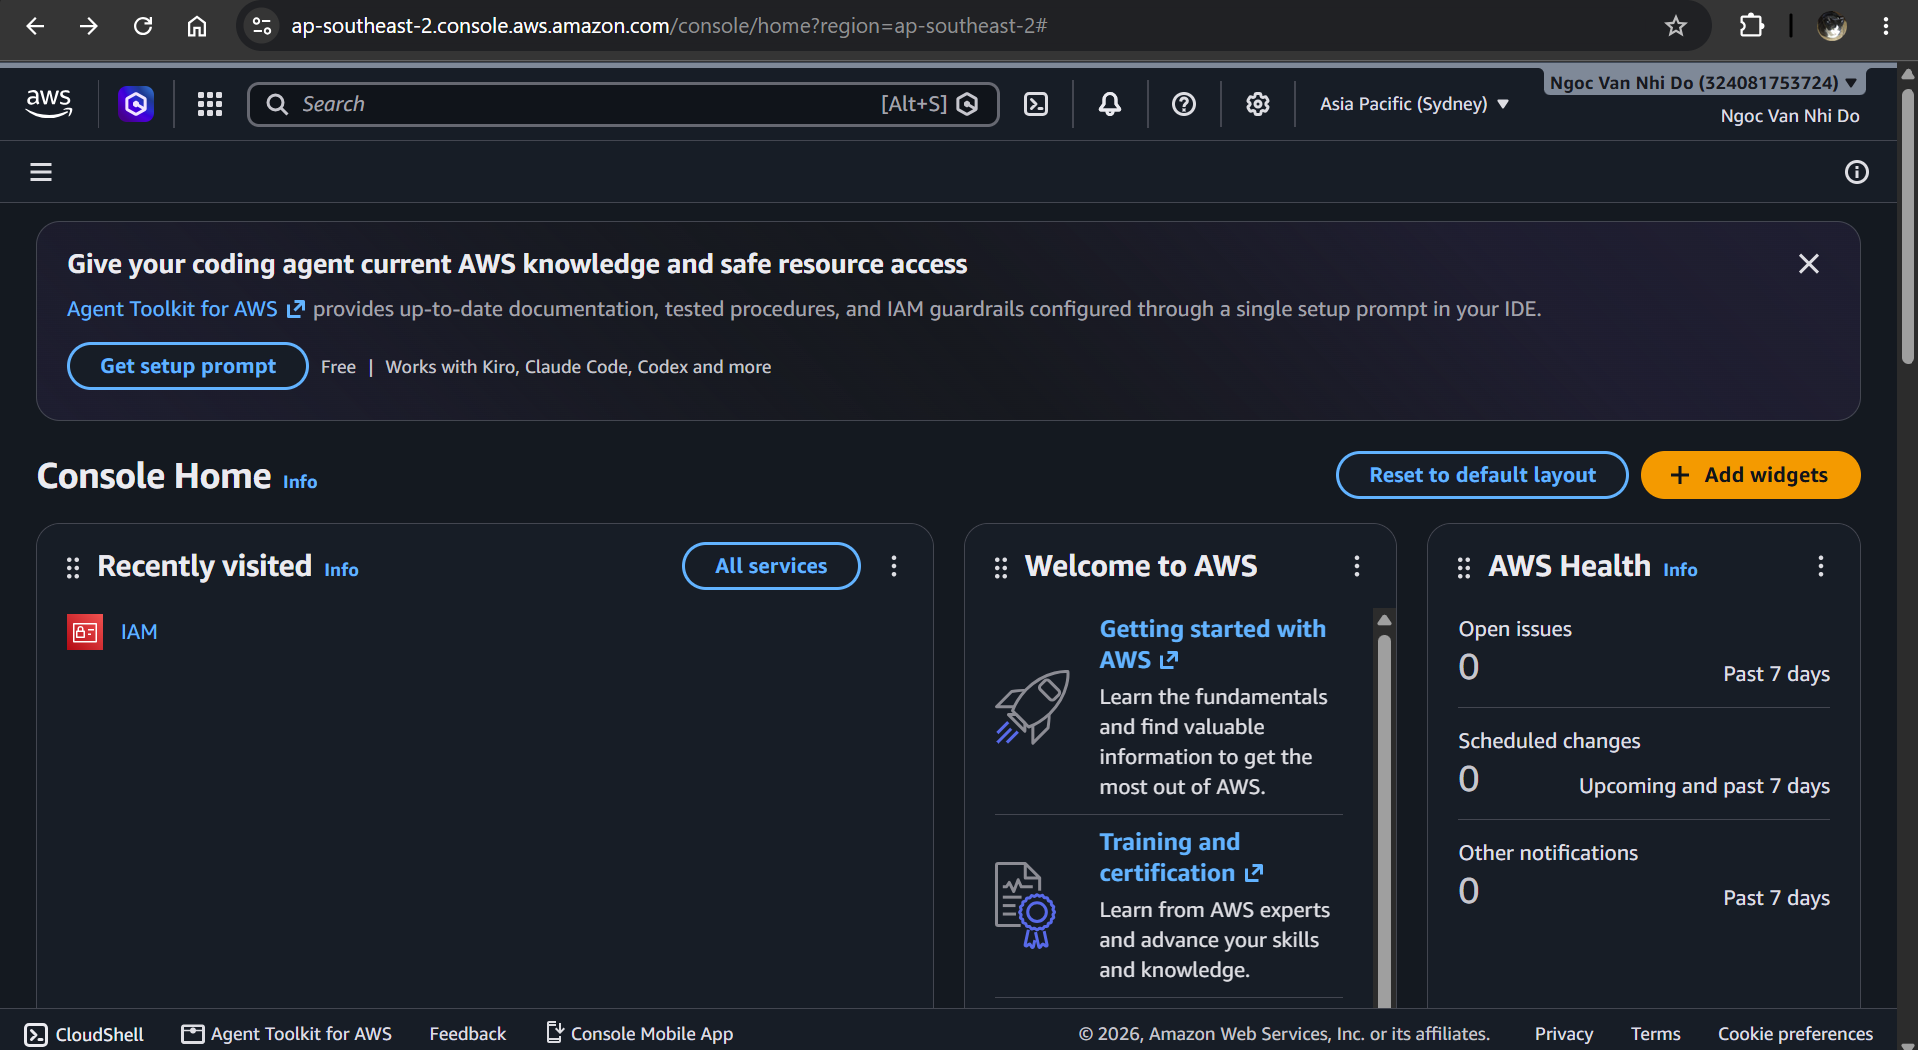
\includegraphics[scale=0.4]{images/1_aws_start.jpg}
\vspace{-1em}
\caption{The AWS Console interface after I had successfully signed up.}
\end{figure}

I then created a new IAM user for my coursework named \texttt{SWE40006\_student} rather than using the root account. This user is assigned to a new user group \texttt{EC2-Lab-Users} which is given full access to EC2 resources (using \texttt{AmazonEC2FullAccess}).

\begin{figure}[H]
\centering
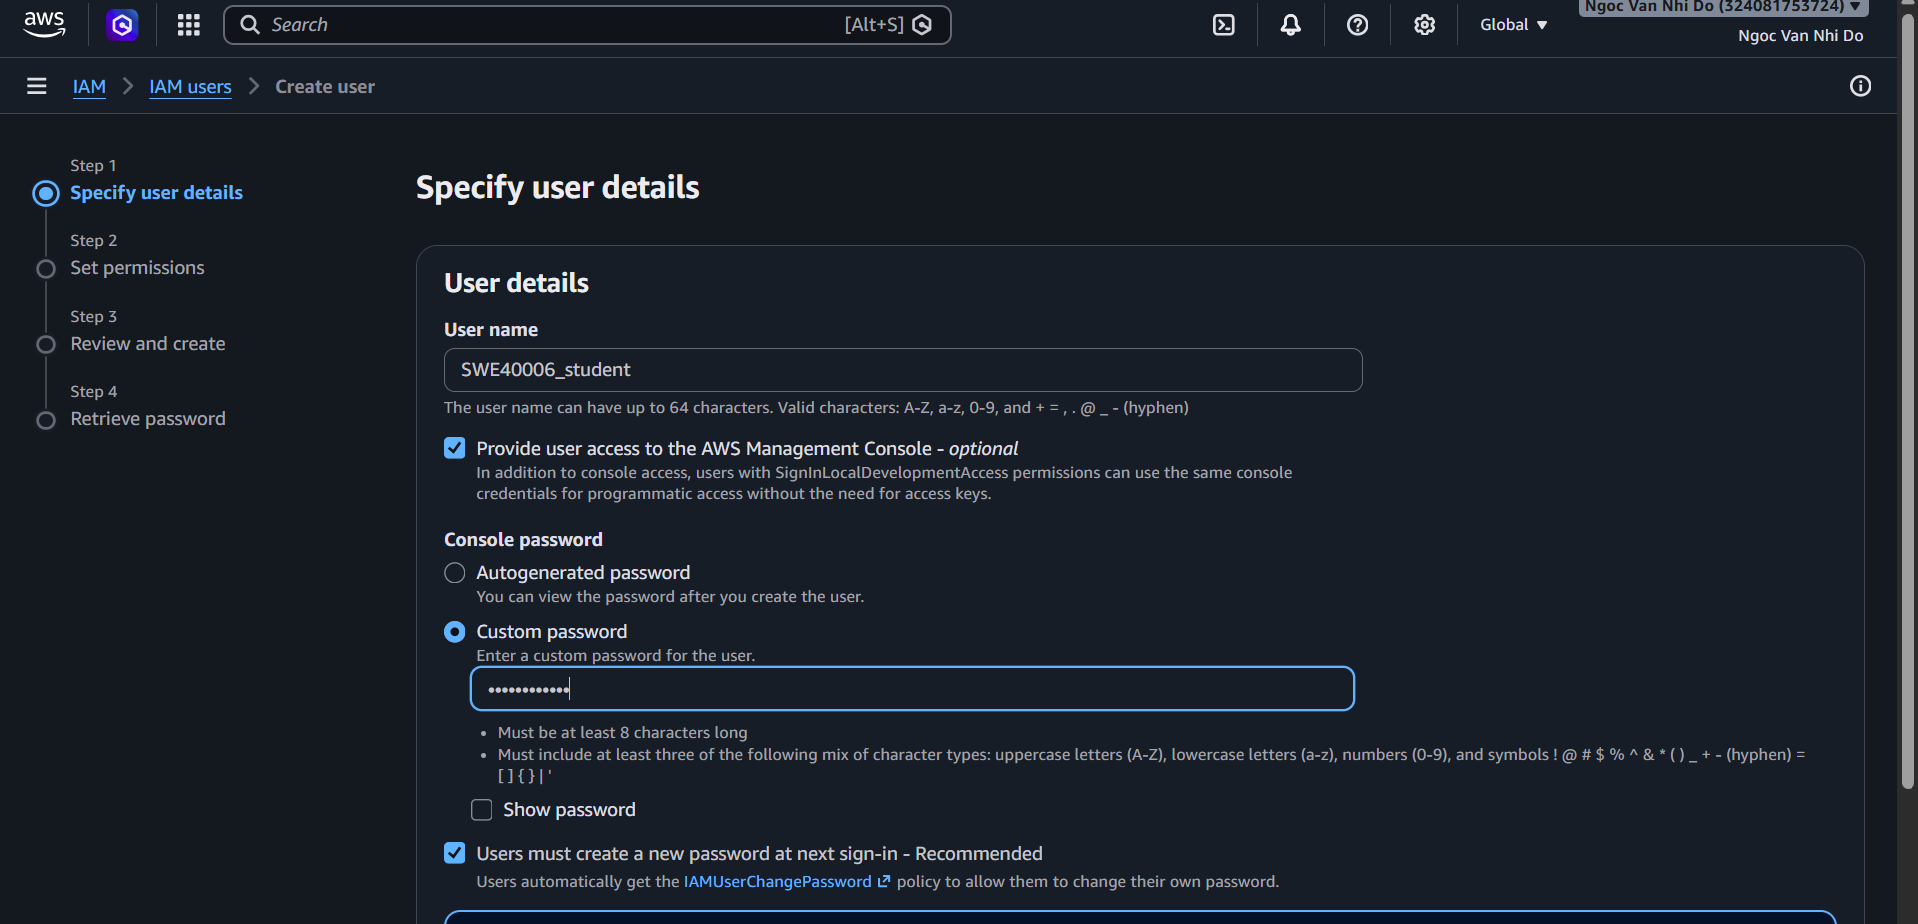
\includegraphics[scale=0.4]{images/1_create_iam.jpg}
\vspace{-1em}
\caption{Creating a new IAM user \texttt{SWE40006\_student}.}
\end{figure}

\begin{figure}[H]
\centering
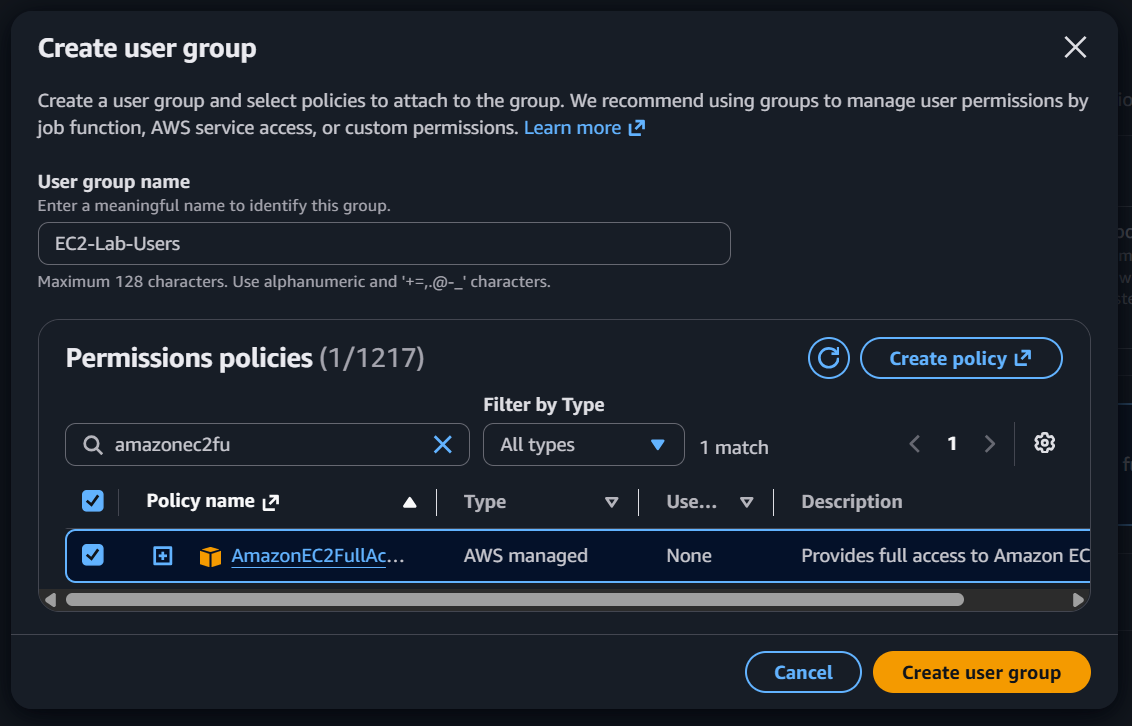
\includegraphics[scale=0.4]{images/1_add_ec2_perms.jpg}
\vspace{-1em}
\caption{Adding \texttt{AmazonEC2FullAccess} to the user group \texttt{EC2-Lab-Users}, which is then assigned to \texttt{SWE40006\_student}.}
\end{figure}

\begin{figure}[H]
\centering
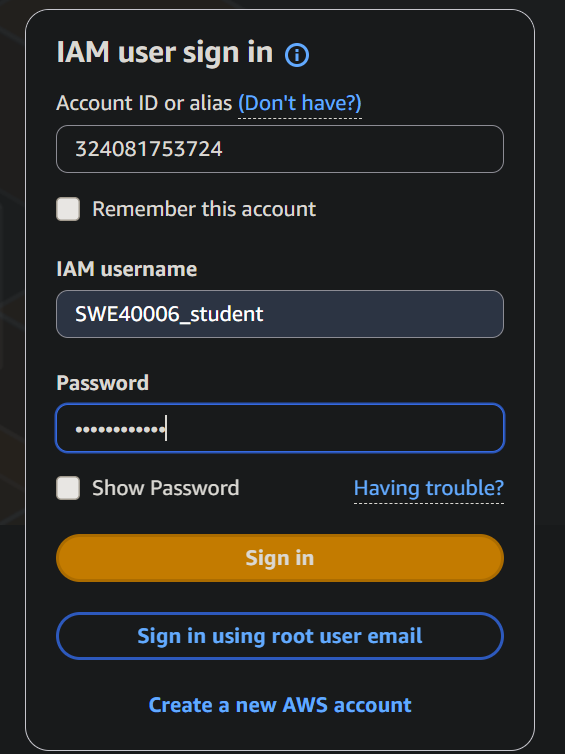
\includegraphics[scale=0.5]{images/1_login_iam.jpg}
\vspace{-1em}
\caption{Logging into the AWS Console as the new IAM user.}
\end{figure}

To securely login into my EC2 instances, I must generate an SSH key pair. The private key was downloaded and stored on my local machine for later authentication.

\begin{figure}[H]
\centering
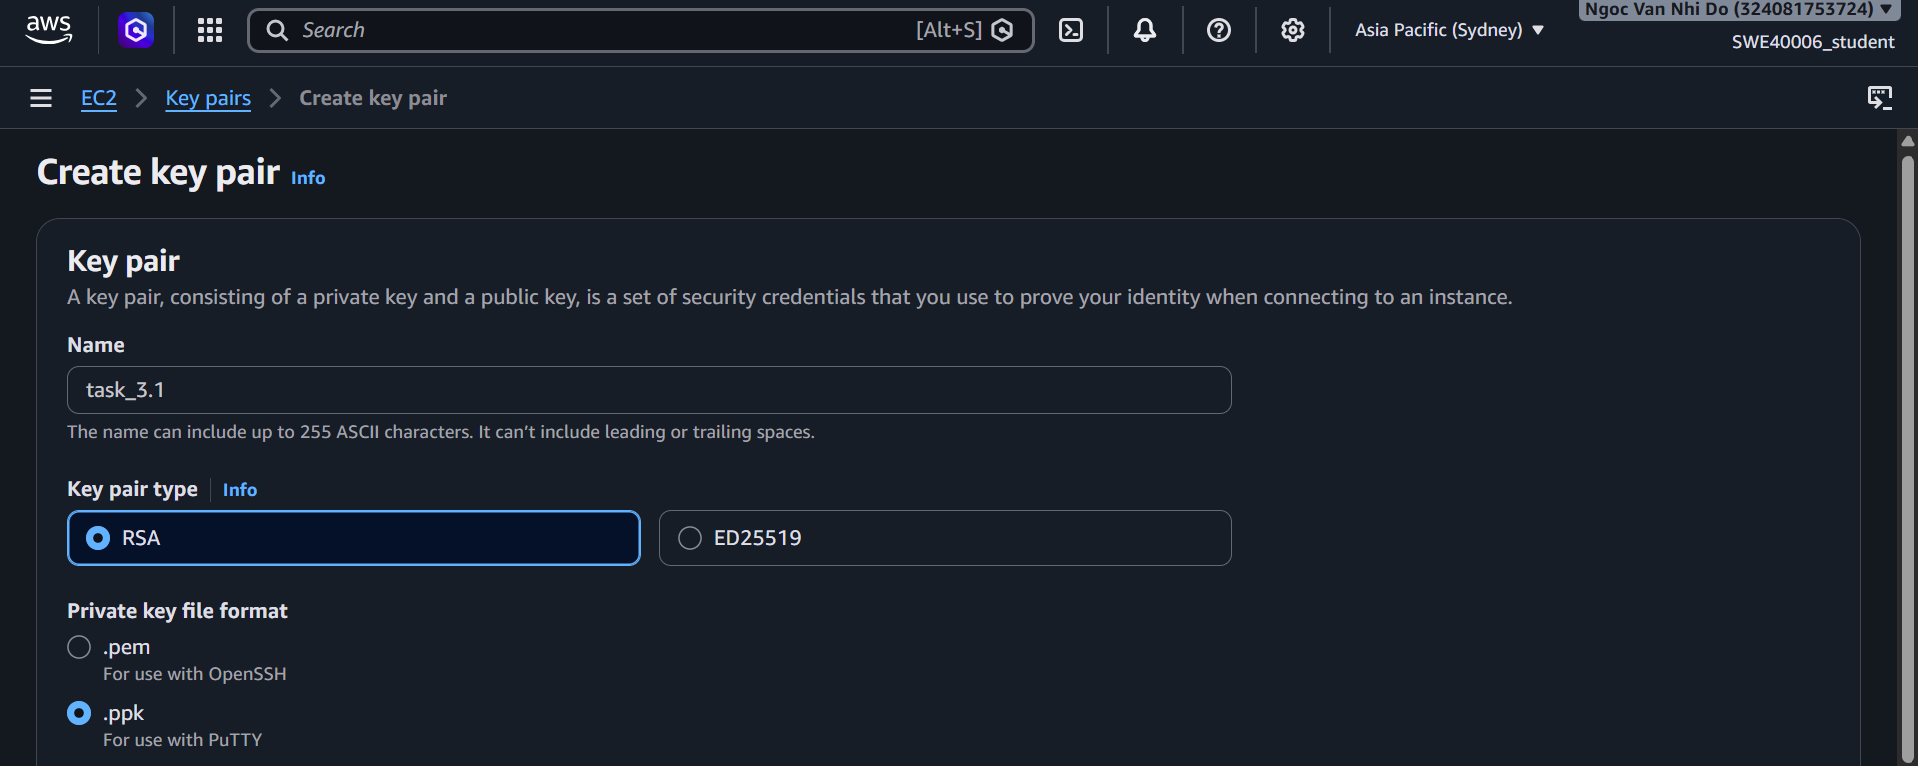
\includegraphics[scale=0.4]{images/1_create_key_pair.jpg}
\vspace{-1em}
\caption{Creating a new key pair \texttt{task-3.1}.}
\end{figure}

\subsubsection{Compute Provisioning}

I launched a new EC2 instance called \texttt{Task 3.1}. This instance runs Amazon Linux 2023, uses a \texttt{t3.micro} instance time to remain eligible for the free tier, and is configured with the previously generated key pair.

\begin{figure}[H]
\centering
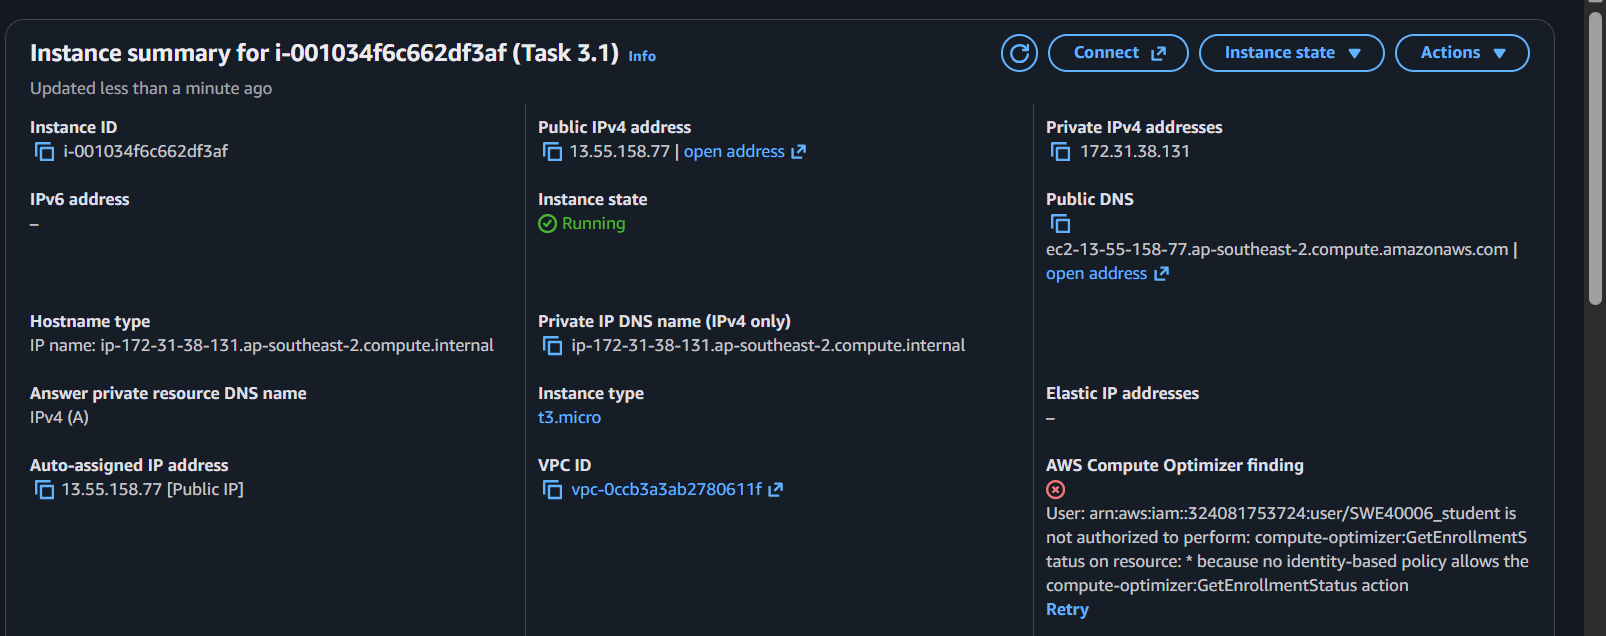
\includegraphics[scale=0.5]{images/1_created_instance.jpg}
\vspace{-1em}
\caption{Creating a new Amazon EC2 instance.}
\end{figure}

\begin{figure}[H]
\centering
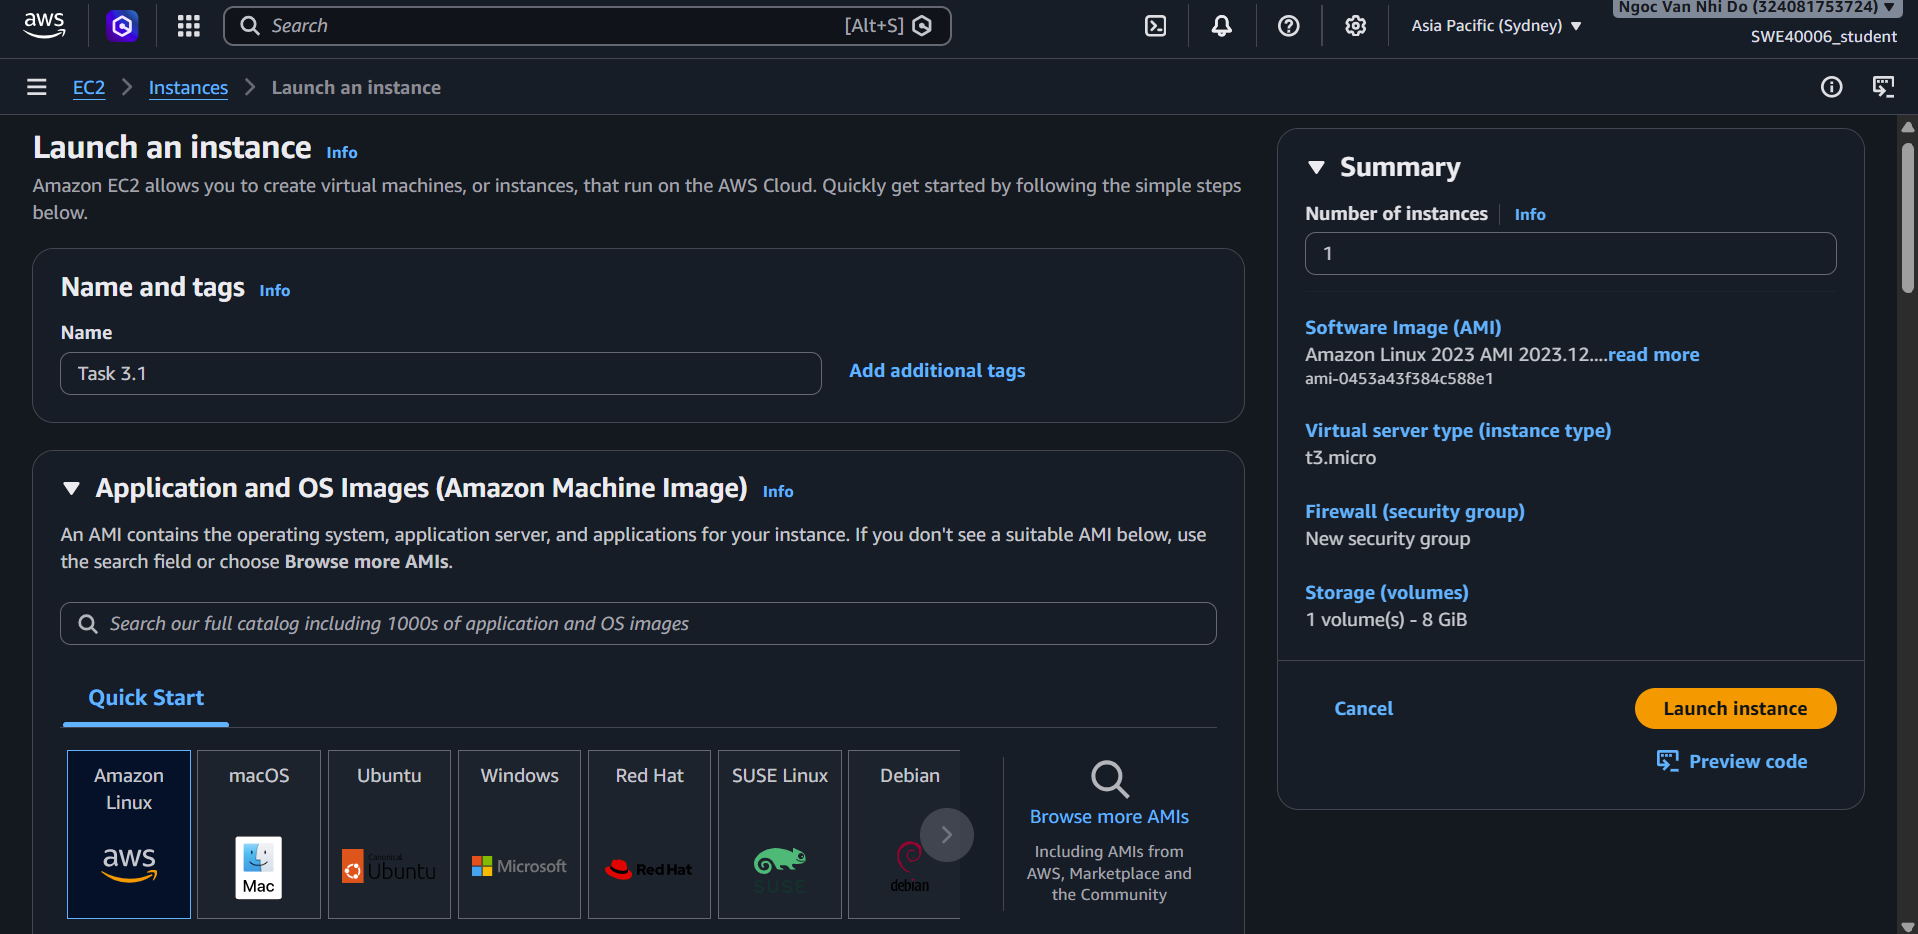
\includegraphics[scale=0.4]{images/1_select_os.jpg}
\vspace{-1em}
\caption{Amazon Linux 2023 was chosen as the OS for this instance.}
\end{figure}

\begin{figure}[H]
\centering
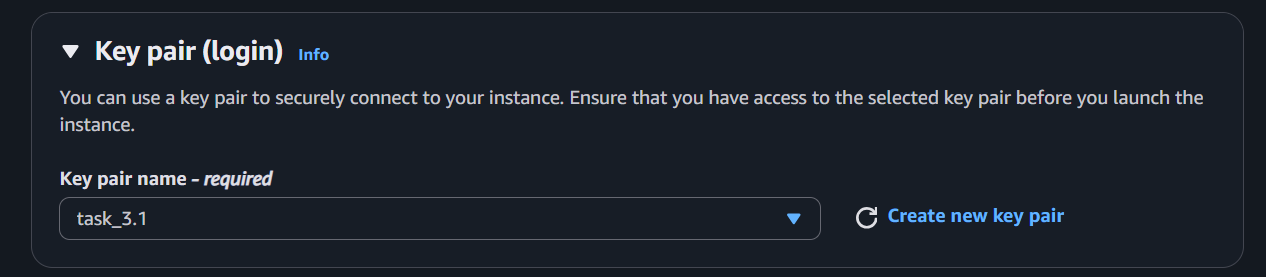
\includegraphics[scale=0.5]{images/1_select_key_pair.jpg}
\vspace{-1em}
\caption{Configuring the instance with the \texttt{task-3.1} key pair.}
\end{figure}

I then configured the instance with a new security group \texttt{task-3.1-sg}, which allowed SSH (22), HTTP (80), and HTTPS (443) inbound traffic from anywhere.

\begin{figure}[H]
\centering
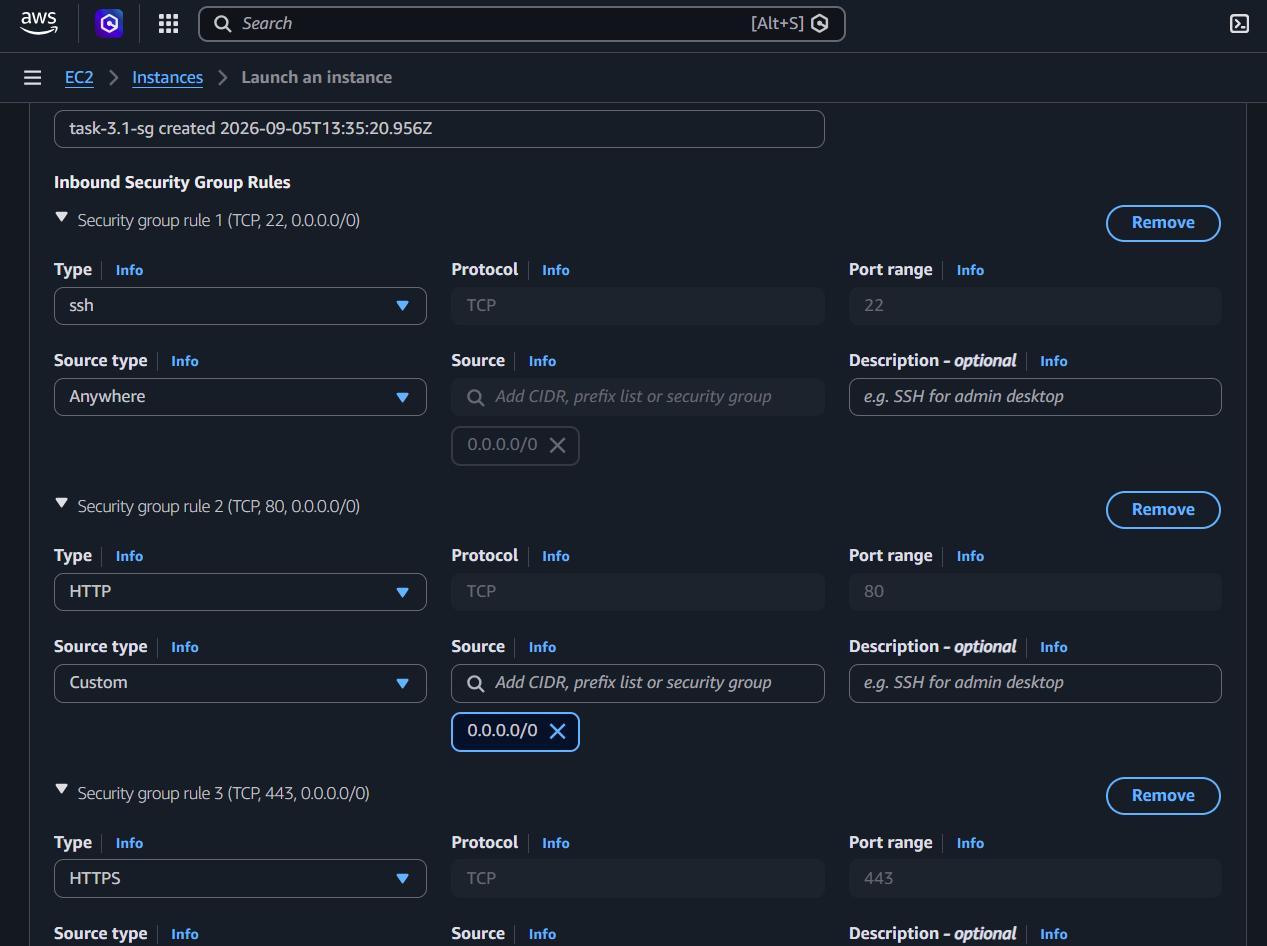
\includegraphics[scale=0.5]{images/1_select_sg.jpg}
\vspace{-1em}
\caption{Configuring the security rules to allow inbound SSH, HTTP, and HTTPS traffic to this instance.}
\end{figure}

\begin{figure}[H]
\centering
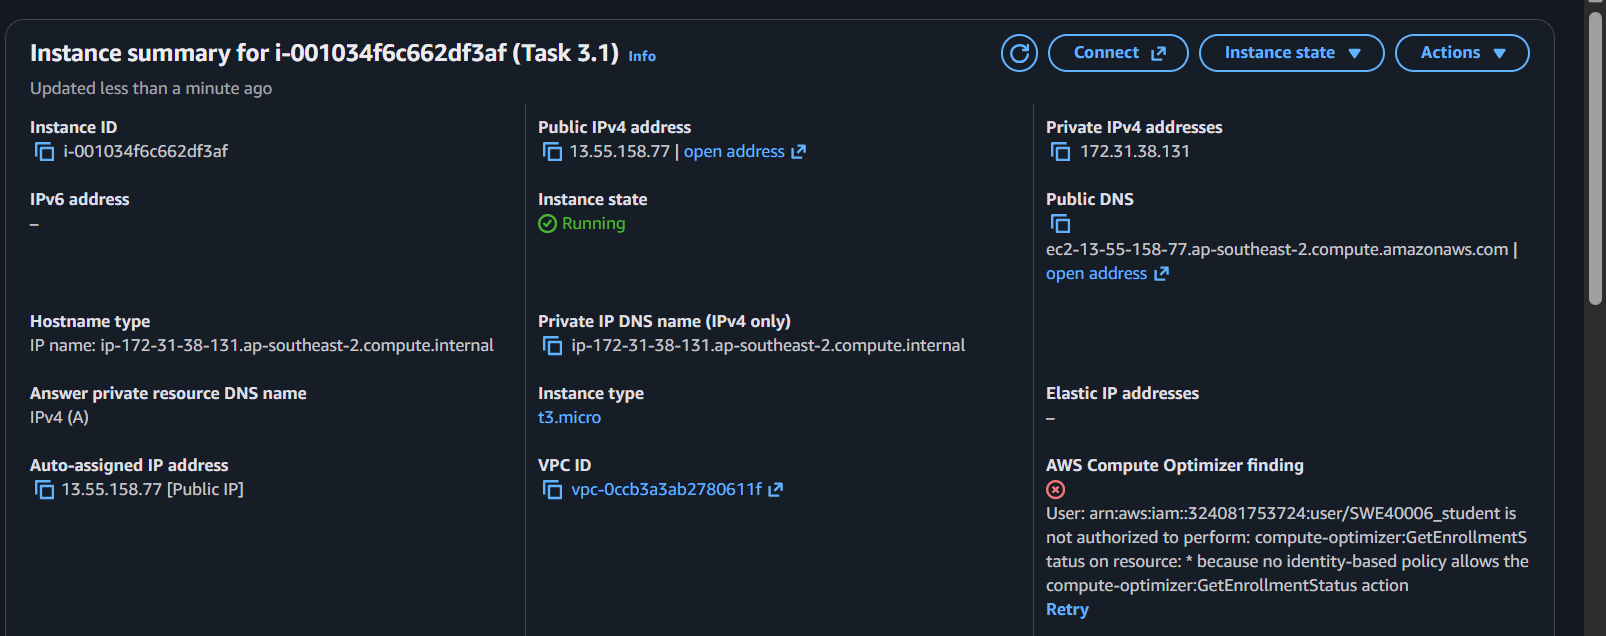
\includegraphics[scale=0.4]{images/1_created_instance.jpg}
\vspace{-1em}
\caption{The new instance is successfully created.}
\end{figure}

I then SSH-ed to the instance using PuTTY.

\begin{figure}[H]
\centering
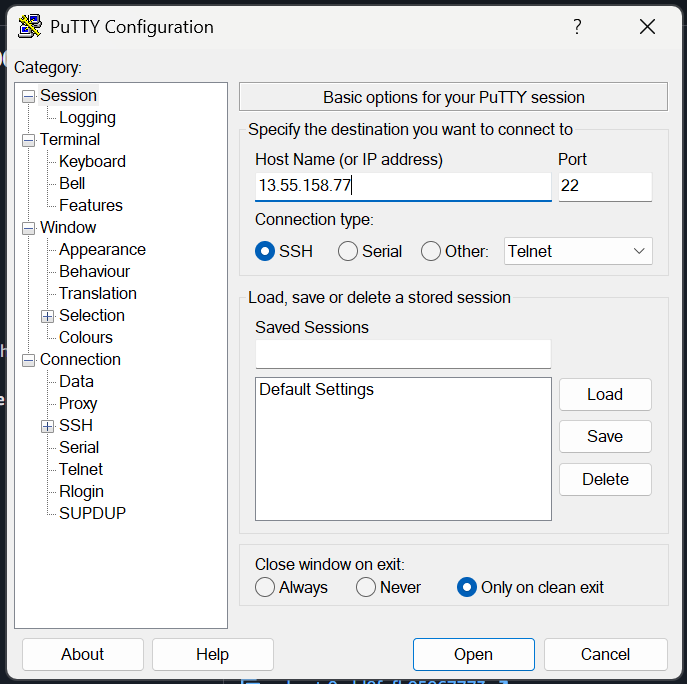
\includegraphics[scale=0.5]{images/1_ssh_ip.jpg}
\vspace{-1em}
\end{figure}

\begin{figure}[H]
\centering
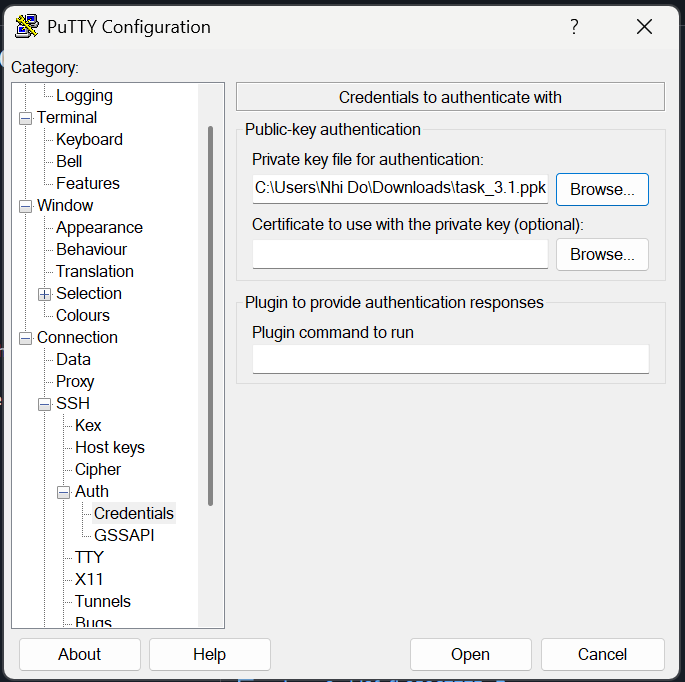
\includegraphics[scale=0.5]{images/1_ssh_key_pair.jpg}
\vspace{-1em}
\caption{Connecting to the EC2 instance using SSH.}
\end{figure}

\begin{figure}[H]
\centering
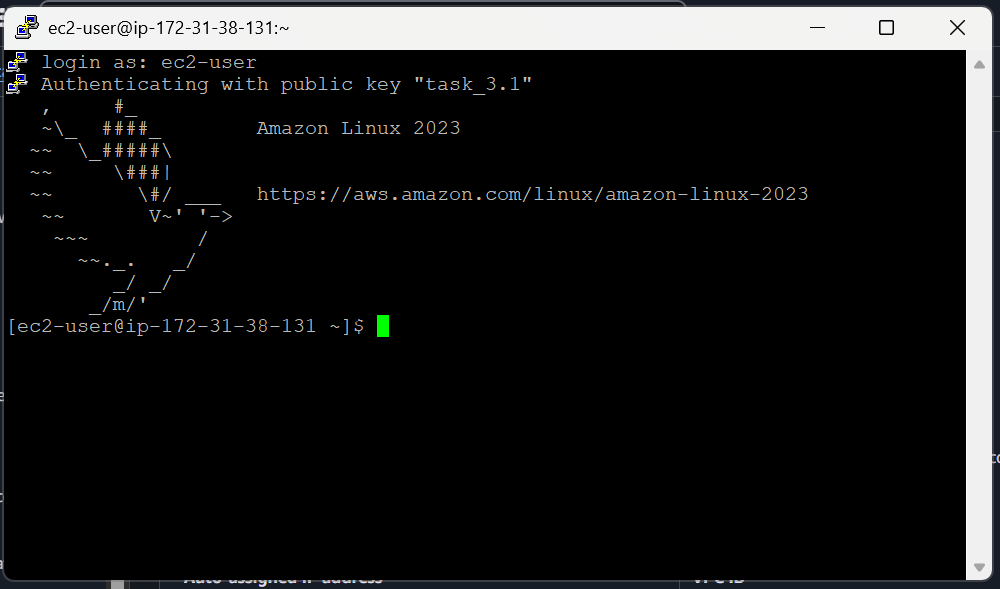
\includegraphics[scale=0.5]{images/1_ssh_success.jpg}
\vspace{-1em}
\caption{Connection was successful.}
\end{figure}

I then installed the Apache web server and started it so that it could later host my web application.

\begin{figure}[H]
\centering
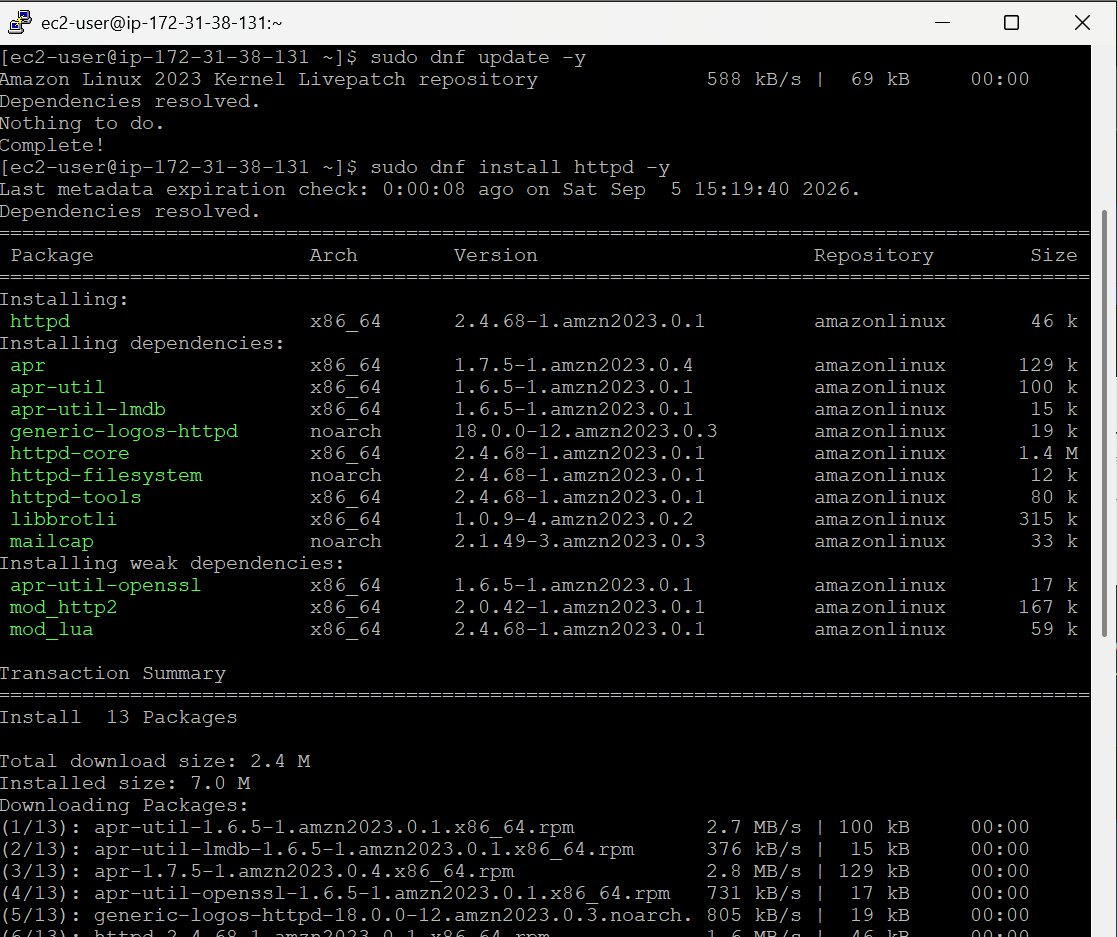
\includegraphics[scale=0.5]{images/1_install_apache.jpg}
\vspace{-1em}
\end{figure}

\begin{figure}[H]
\centering
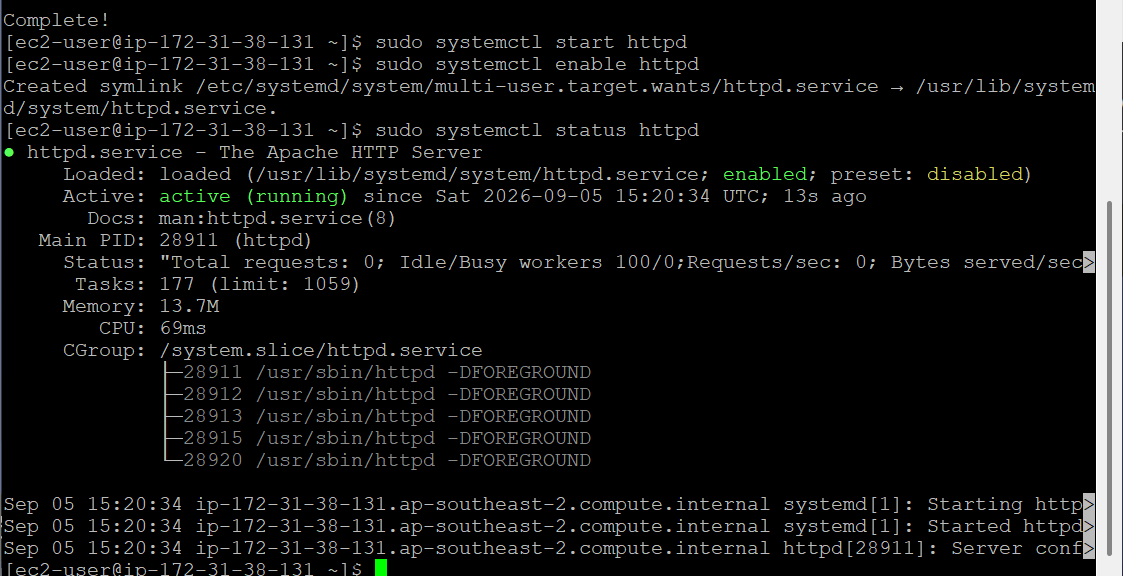
\includegraphics[scale=0.5]{images/1_start_apache.jpg}
\vspace{-1em}
\caption{Installing and starting the web server.}
\end{figure}

\begin{figure}[H]
\centering
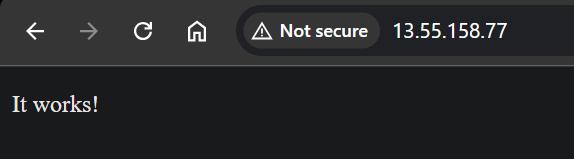
\includegraphics[scale=0.6]{images/1_verify_running.jpg}
\vspace{-1em}
\caption{Verifying that the web server is publicly accessible.}
\end{figure}

\subsubsection{Application Deployment}

Before deploying the WordPress application, I needed to install its dependencies which included installing PHP and MariaDB.

\begin{figure}[H]
\centering
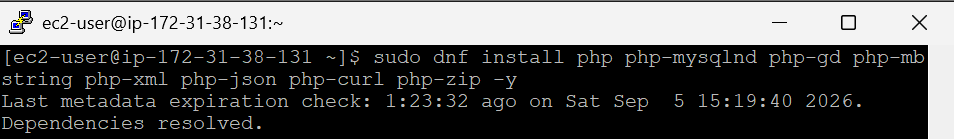
\includegraphics[scale=0.5]{images/1_install_php.jpg}
\vspace{-1em}
\caption{Installing PHP.}
\end{figure}

\begin{figure}[H]
\centering
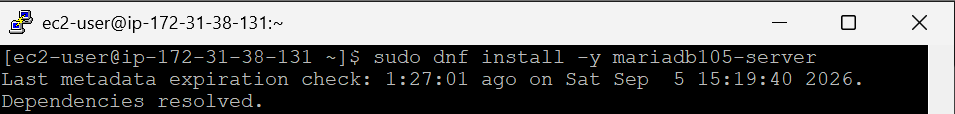
\includegraphics[scale=0.5]{images/1_install_mariadb.jpg}
\vspace{-1em}
\caption{Installing MariaDB.}
\end{figure}

\begin{figure}[H]
\centering
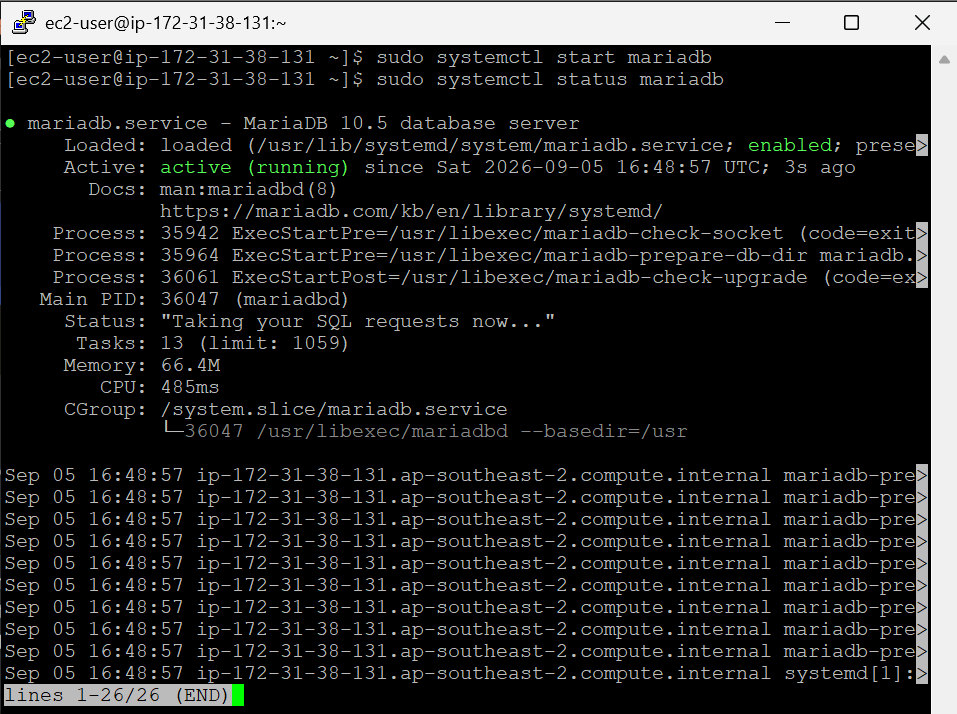
\includegraphics[scale=0.5]{images/1_start_mariadb.jpg}
\vspace{-1em}
\caption{Starting and enabling the MariaDB service.}
\end{figure}

I then set up a local database for the web application.

\begin{figure}[H]
\centering
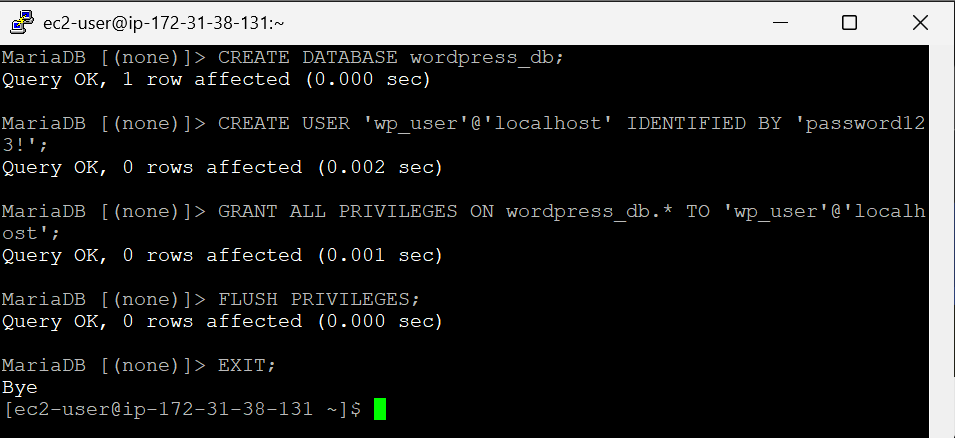
\includegraphics[scale=0.5]{images/1_create_db.jpg}
\vspace{-1em}
\caption{Setting up a local database named \texttt{wordpress\_db} for the WordPress application.}
\end{figure}

I installed and extracted the WordPress package. The command \texttt{chown} made Apache the owner of the WordPress files, while \texttt{chmod} set who could read, write, or access those files. These commands ensured that Apache had the correct permissions to run WordPress.

\begin{figure}[H]
\centering
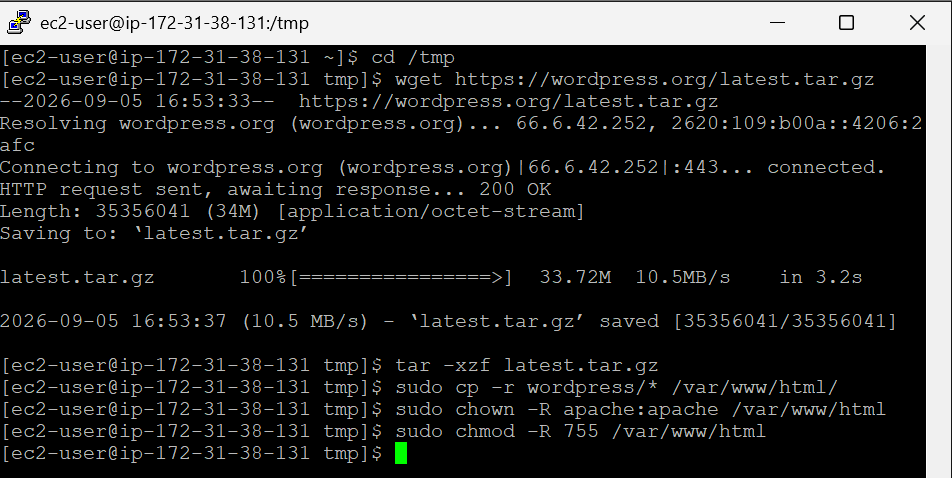
\includegraphics[scale=0.5]{images/1_install_wordpress.jpg}
\vspace{-1em}
\caption{Installing WordPress and configuring permissions.}
\end{figure}

\begin{figure}[H]
\centering
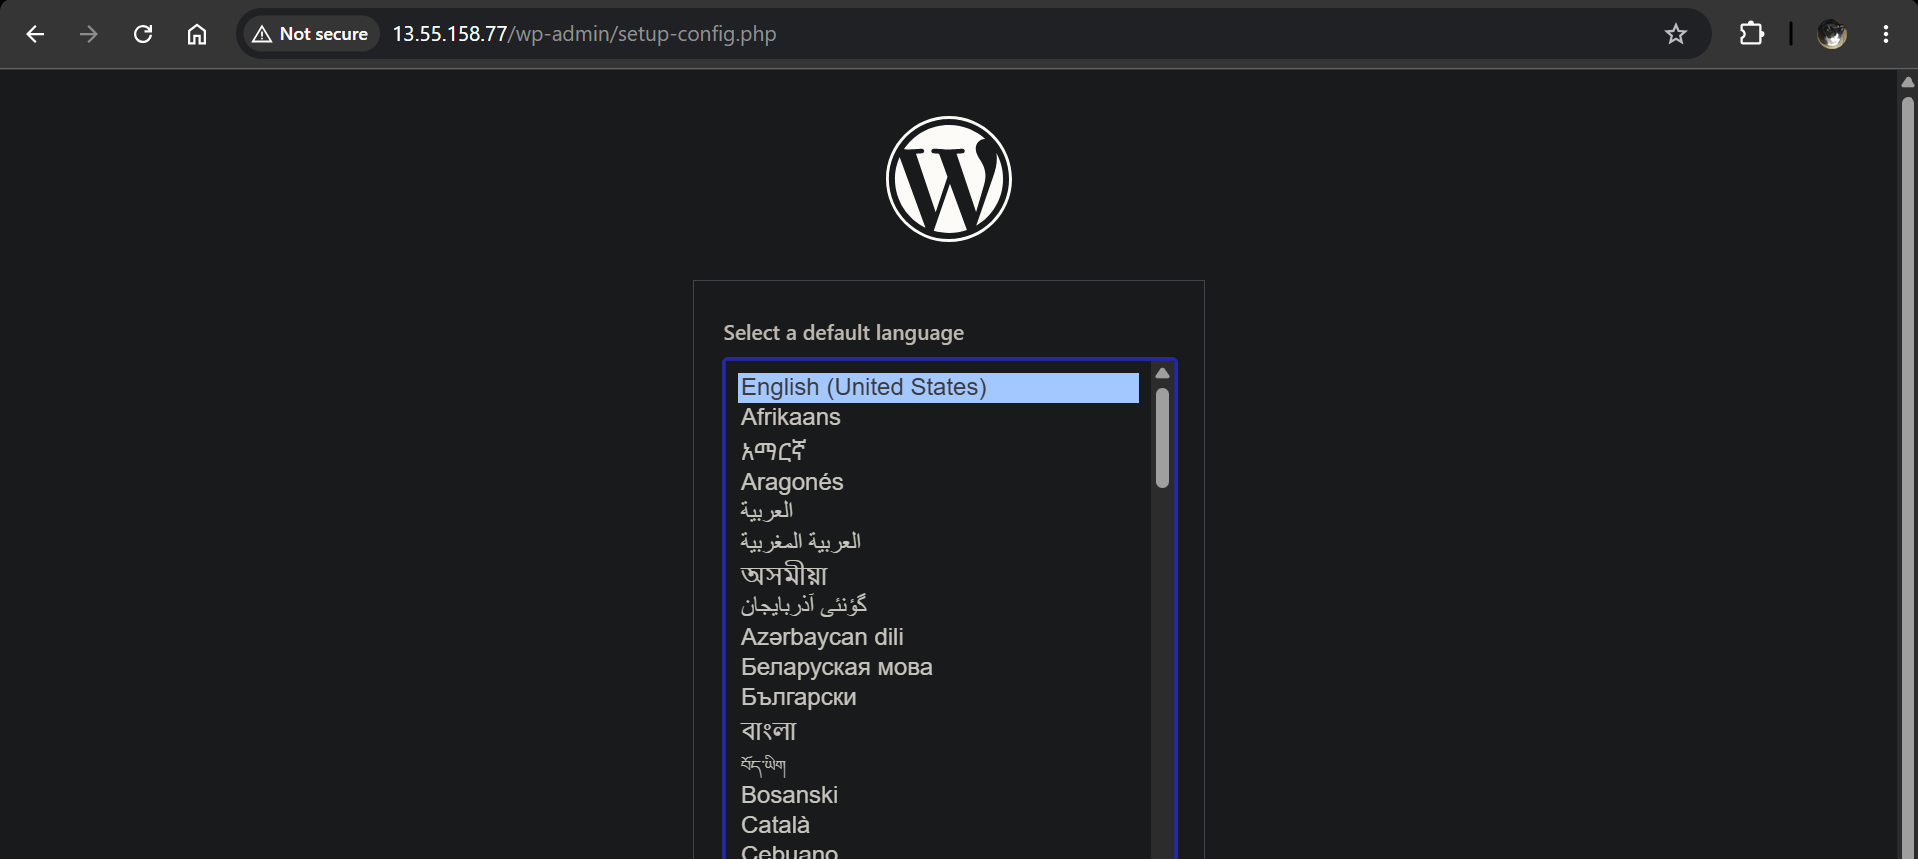
\includegraphics[scale=0.4]{images/1_deployed.jpg}
\vspace{-1em}
\caption{The deployed WordPress application.}
\end{figure}

\subsection{Task 3.2}

For this task, I configured my web application to use a database hosted on an Amazon RDS instance, effectively decoupling the database from the EC2 instance. I also created a backup of my web application by storing my files on an S3 bucket, and demonstrated how I could restore my application using this backup.

\subsubsection{Database Decoupling}

I started by creating a new RDS instance and configured it to use MariaDB as the database engine. I also connected the EC2 instance to this database right away, so that AWS automatically allowed inbound traffic on port 3306 from the web application to the database for me.

\begin{figure}[H]
\centering
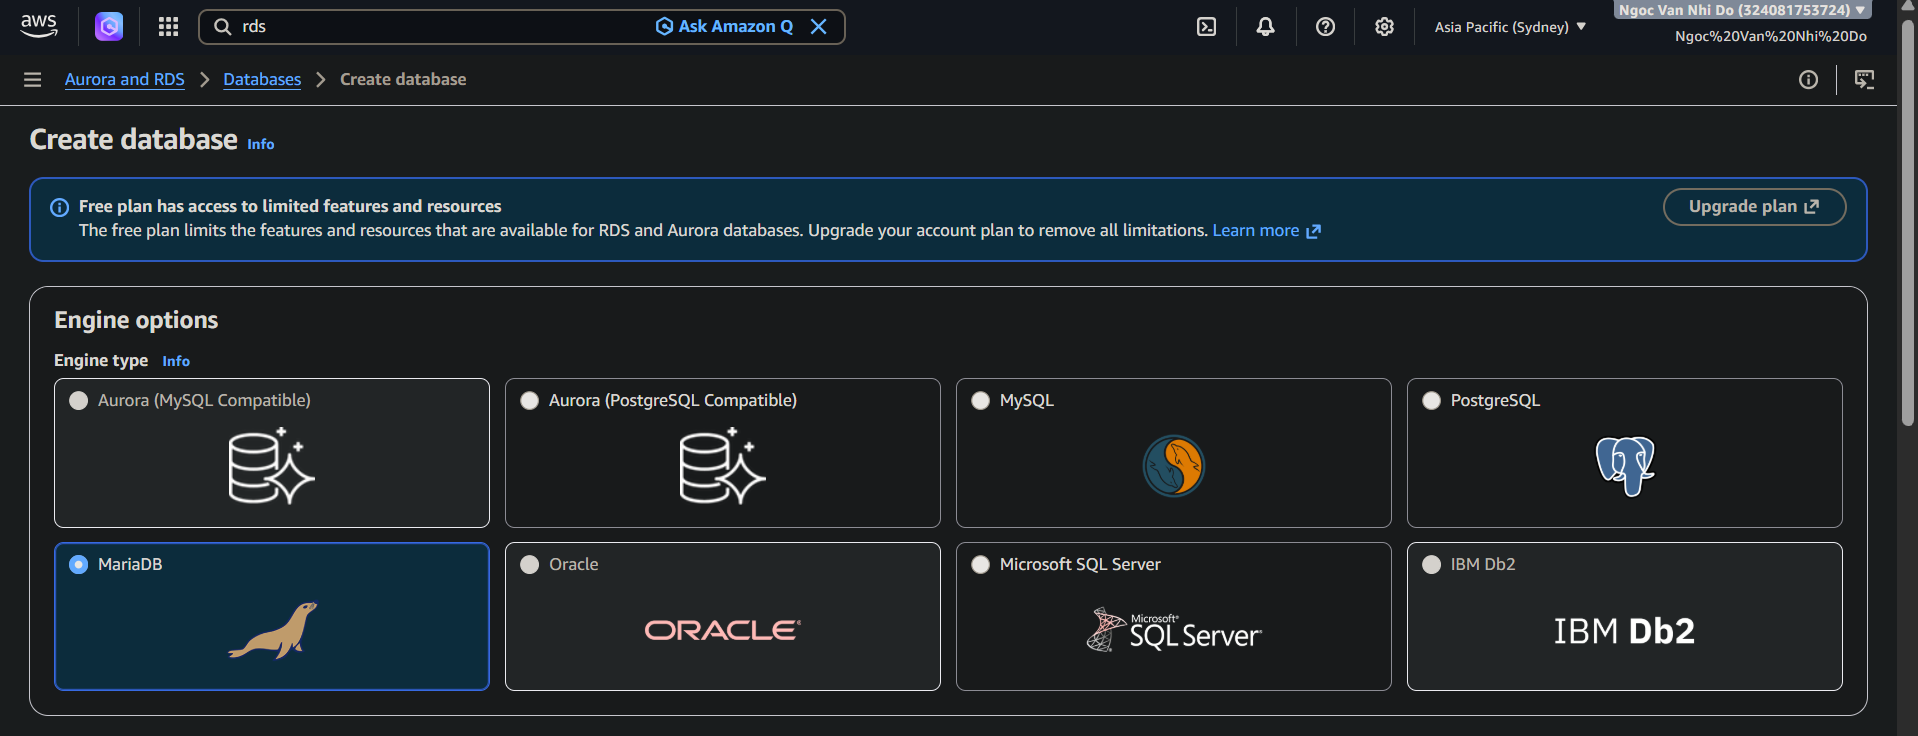
\includegraphics[scale=0.4]{images/2_select_mariadb.jpg}
\vspace{-1em}
\caption{Creating a new RDS instance.}
\end{figure}

\begin{figure}[H]
\centering
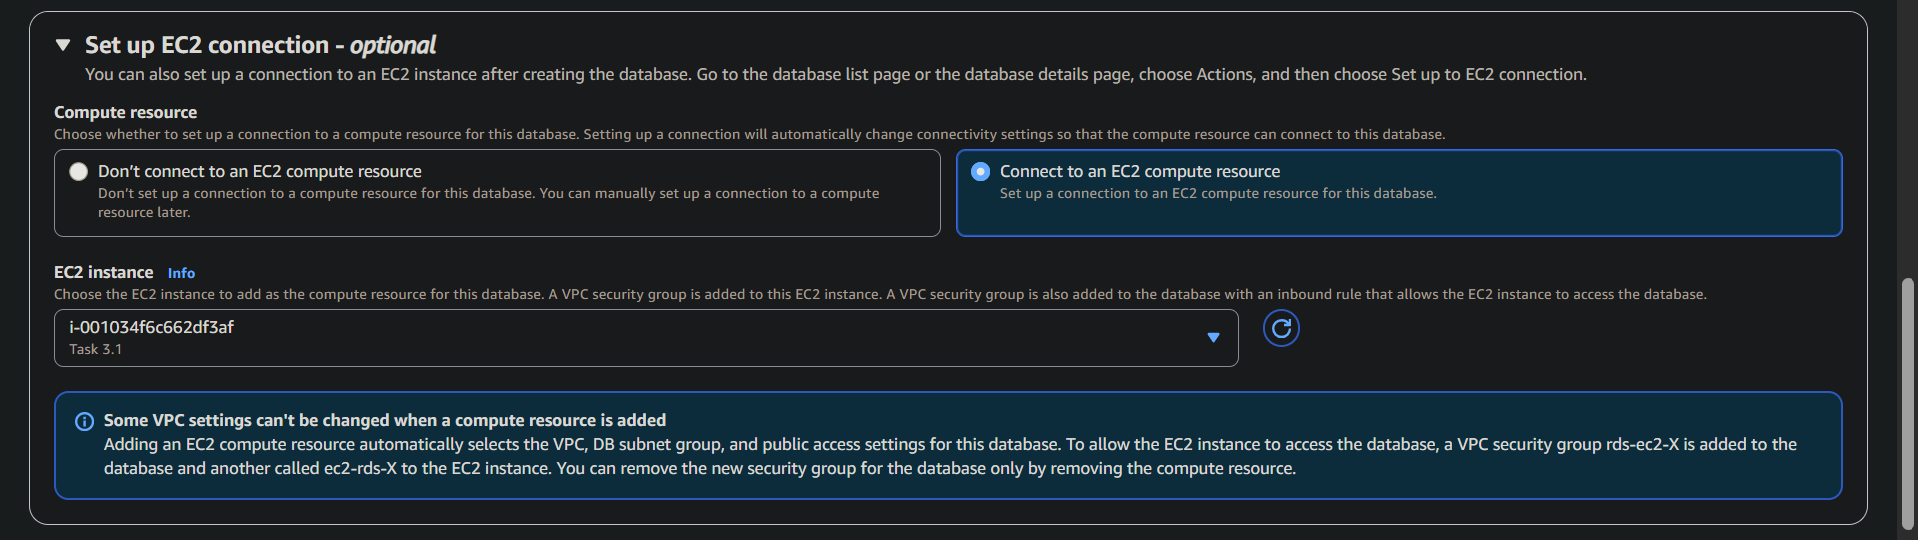
\includegraphics[scale=0.4]{images/2_connect_ec2.jpg}
\vspace{-1em}
\caption{Connecting the EC2 instance from the previous task.}
\end{figure}

\begin{figure}[H]
\centering
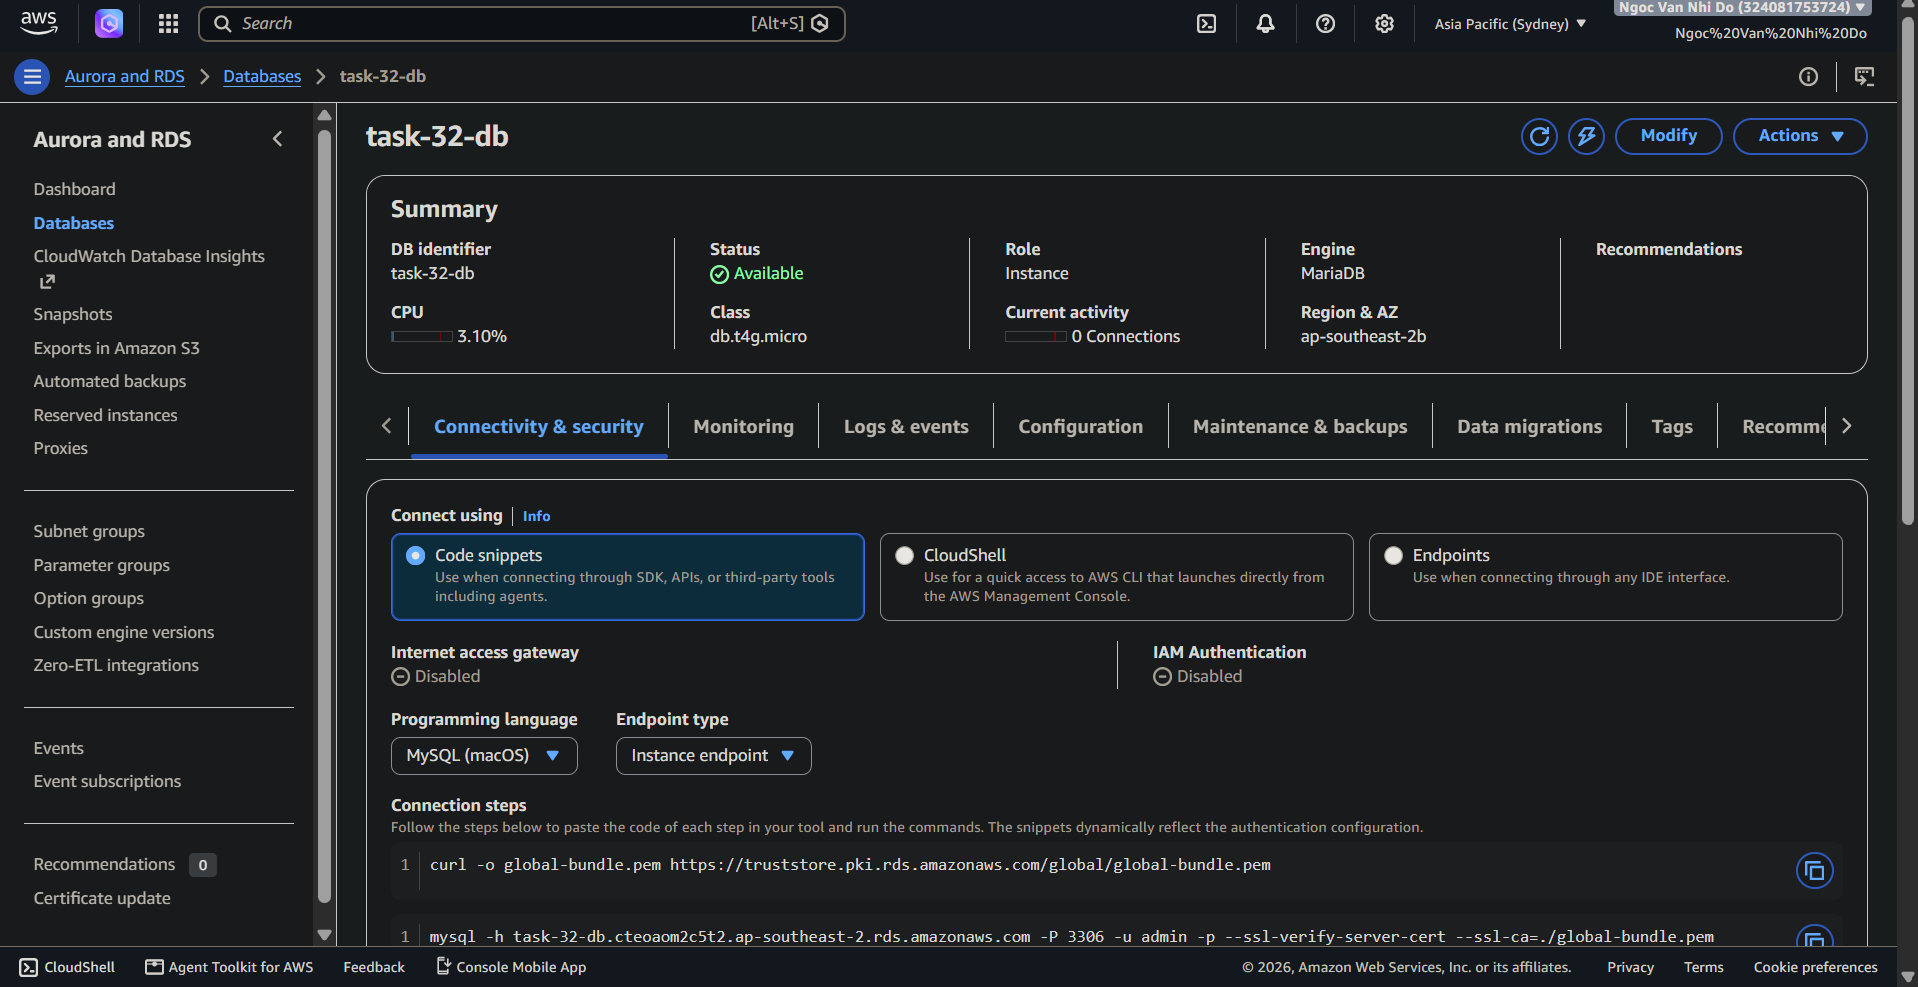
\includegraphics[scale=0.4]{images/2_db_created.jpg}
\vspace{-1em}
\caption{The database is successfully created.}
\end{figure}

From the EC2 instance's command line, I established a connection to the RDS instance using its endpoint at \url{task-32-db.cteoaom2c5t2.ap-southeast-2.rds.amazonaws.com}. 

\begin{figure}[H]
\centering
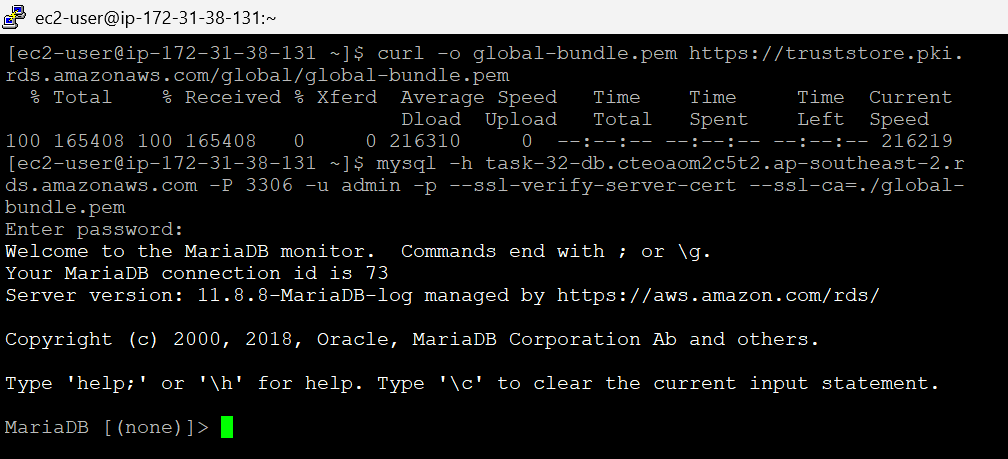
\includegraphics[scale=0.5]{images/2_connect_rds.jpg}
\vspace{-1em}
\caption{Connecting to the database from the EC2 instance's terminal.}
\end{figure}

Once I could connect to the database, I created a new database \texttt{wordpress\_db} to be used by my application. I then exited the DB connection, configured the \texttt[wg\_config.php] file with the required database information, including the database name, username, and password, along with the other necessary credentials. This allowed the WordPress application to connect to and use the configured database. Finally, I restarted the Apache web server and verified that the application has been successfully configured to use the database. As I had not installed the actual WordPress application by this point, the database displayed all empty entries.

\begin{figure}[H]
\centering
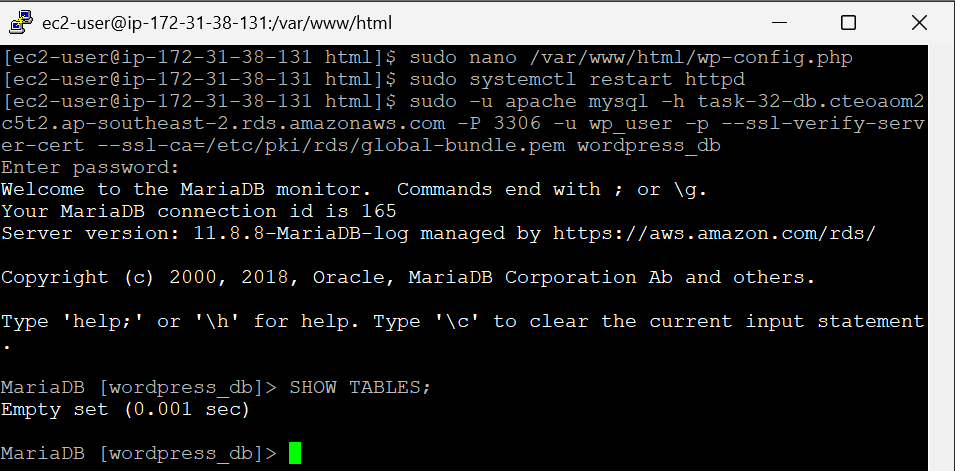
\includegraphics[scale=0.5]{images/2_config_db.jpg}
\end{figure}

\begin{figure}[H]
\centering
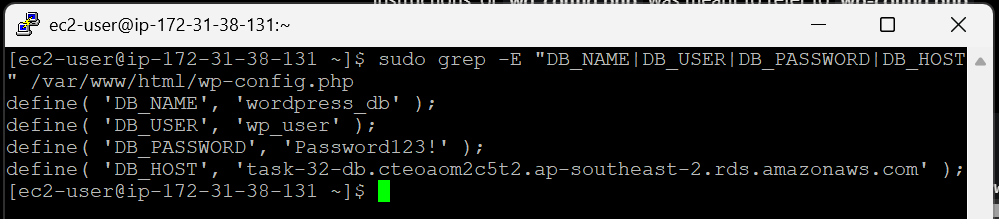
\includegraphics[scale=0.5]{images/2_db_configs.jpg}
\vspace{-1em}
\caption{Editing the database configurations and verifiying the connection to the RDS database.}
\end{figure}

\begin{figure}[H]
\centering
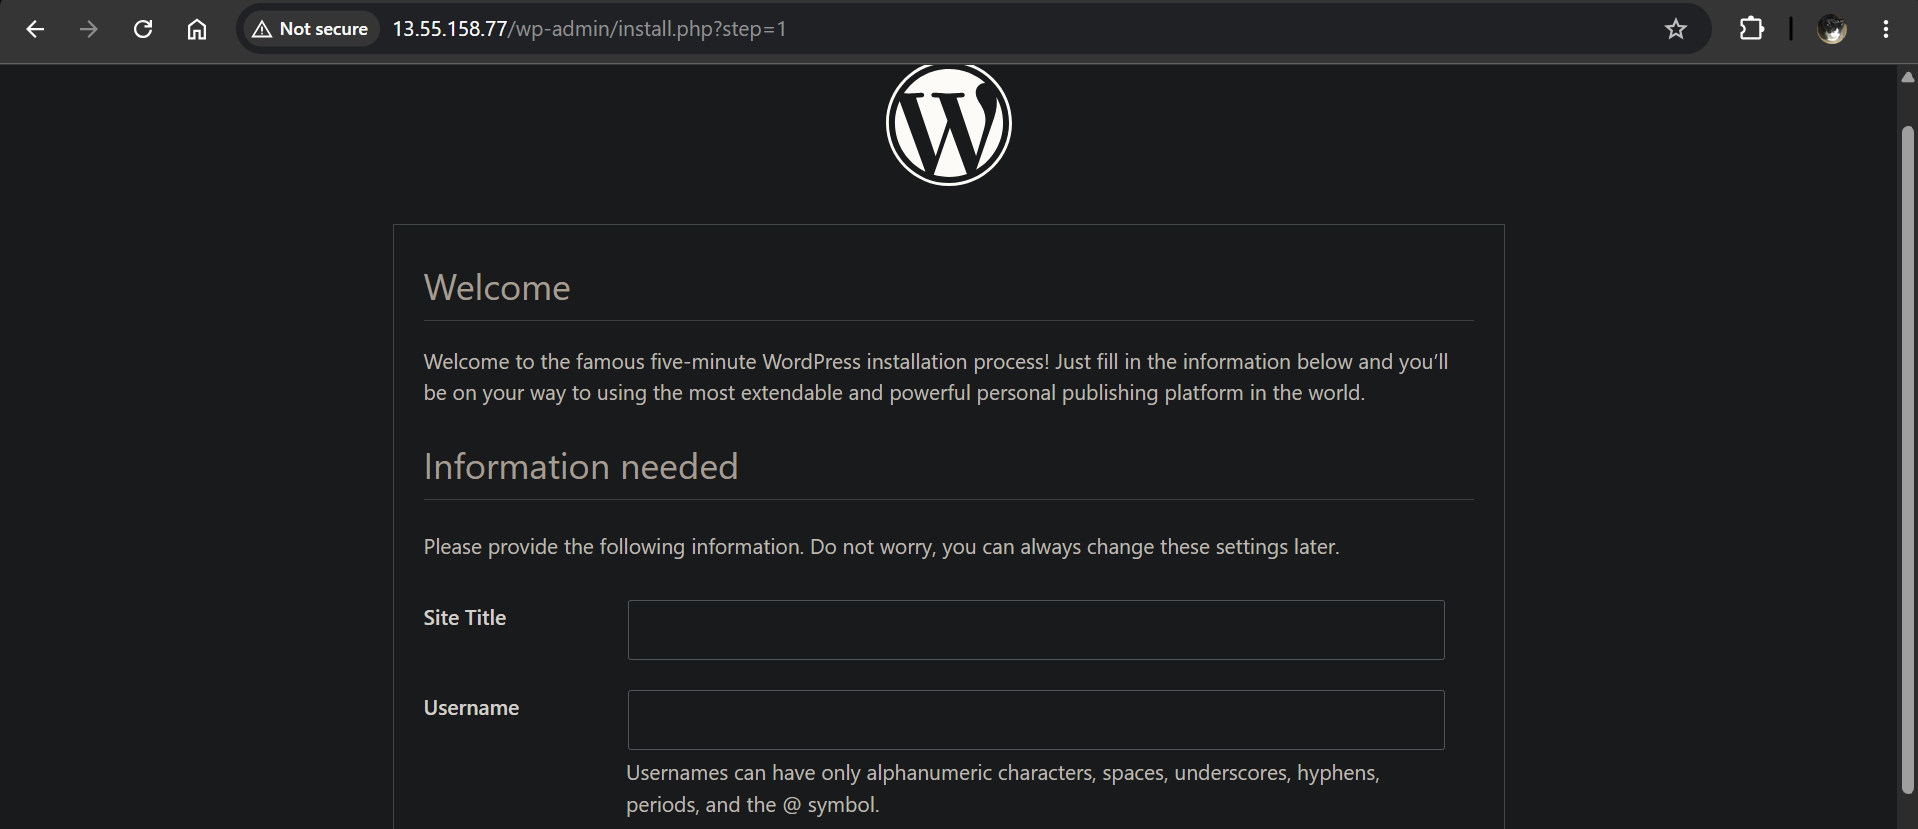
\includegraphics[scale=0.4]{images/2_db_configured.jpg}
\vspace{-1em}
\caption{The application now shows the WordPress installation form, which means the database has successfully been connected.}
\end{figure}

\subsubsection{Backup and Restore}

I started by creating a new S3 bucket with the name \texttt{swe40006-105551765-bucket} to store my backup files.

\begin{figure}[H]
\centering
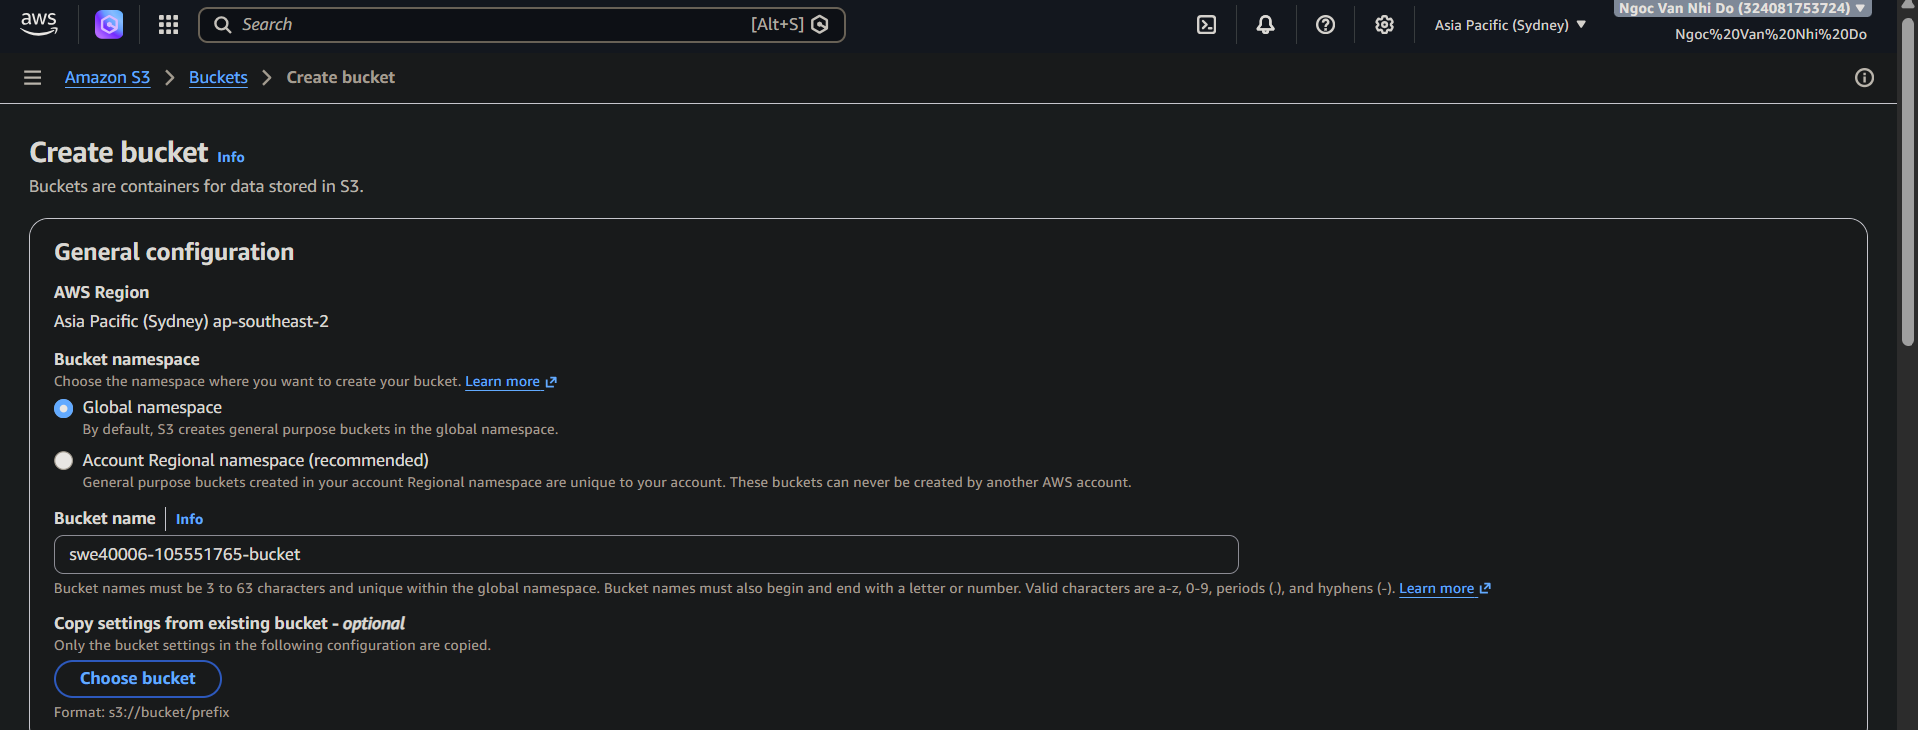
\includegraphics[scale=0.4]{images/2_create_bucket.jpg}
\vspace{-1em}
\caption{The application now shows the WordPress installation form, which means the database has successfully been connected.}
\end{figure}

I also created a new IAM role allowing full access to S3. This role is then attached to my EC2 instance so that the server could read and write files to the S3 bucket.

\begin{figure}[H]
\centering
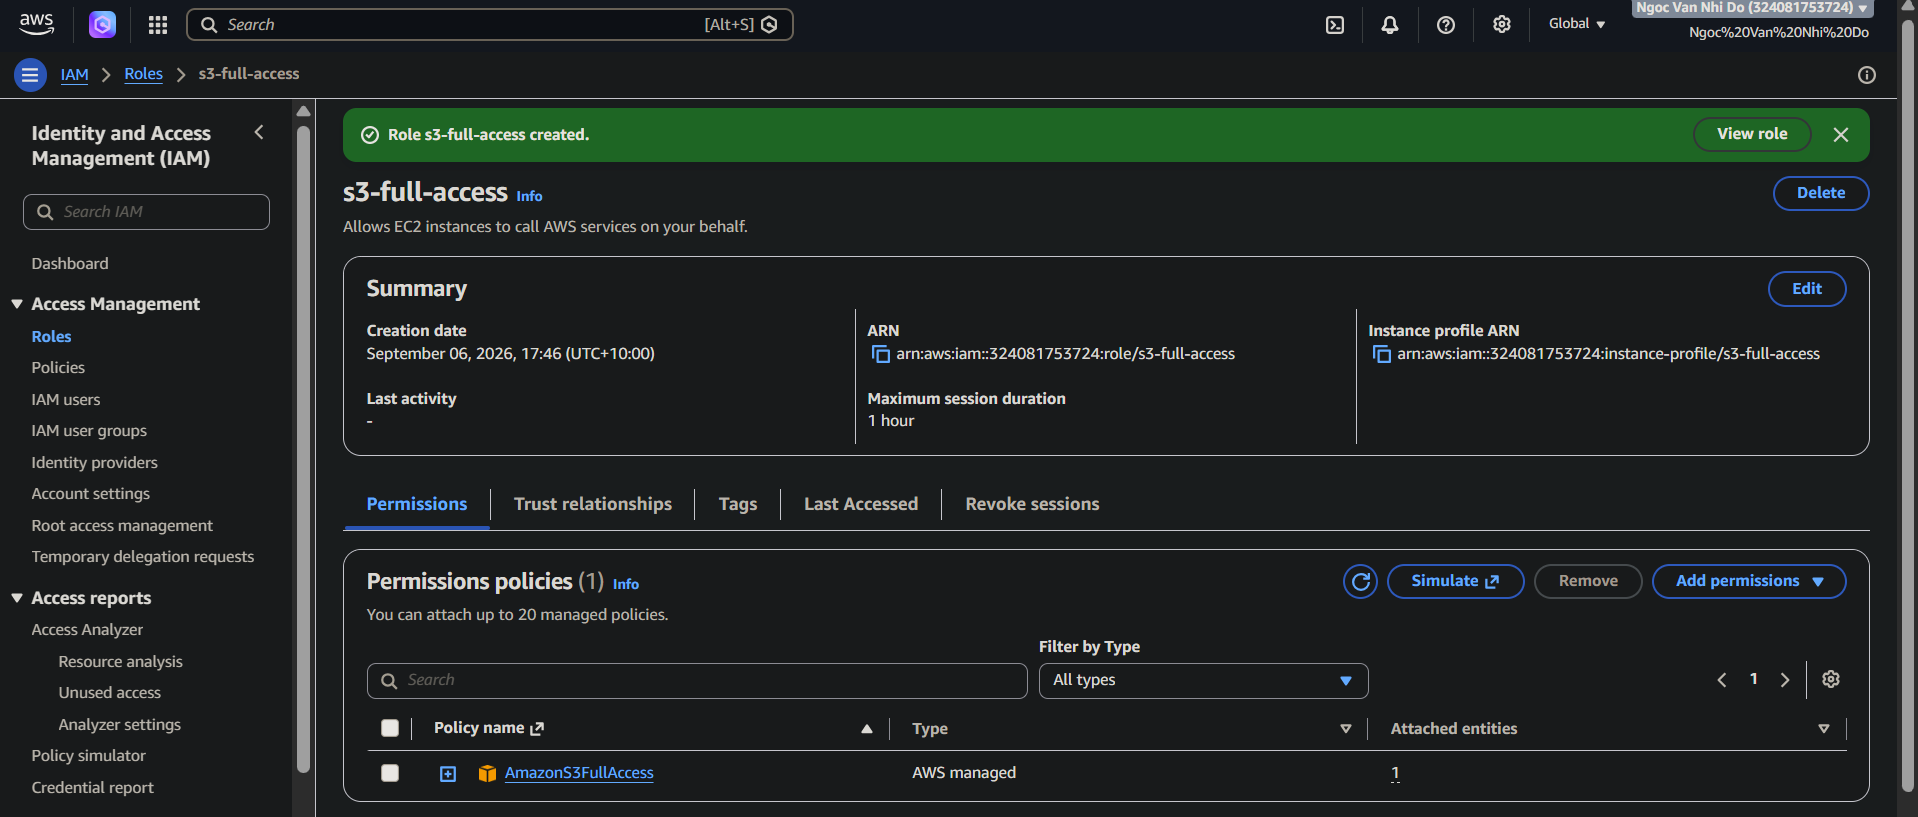
\includegraphics[scale=0.4]{images/2_create_role.jpg}
\vspace{-1em}
\caption{Creating a new IAM role with the \texttt{AmazonS3FullAccess} policy.}
\end{figure}

\begin{figure}[H]
\centering
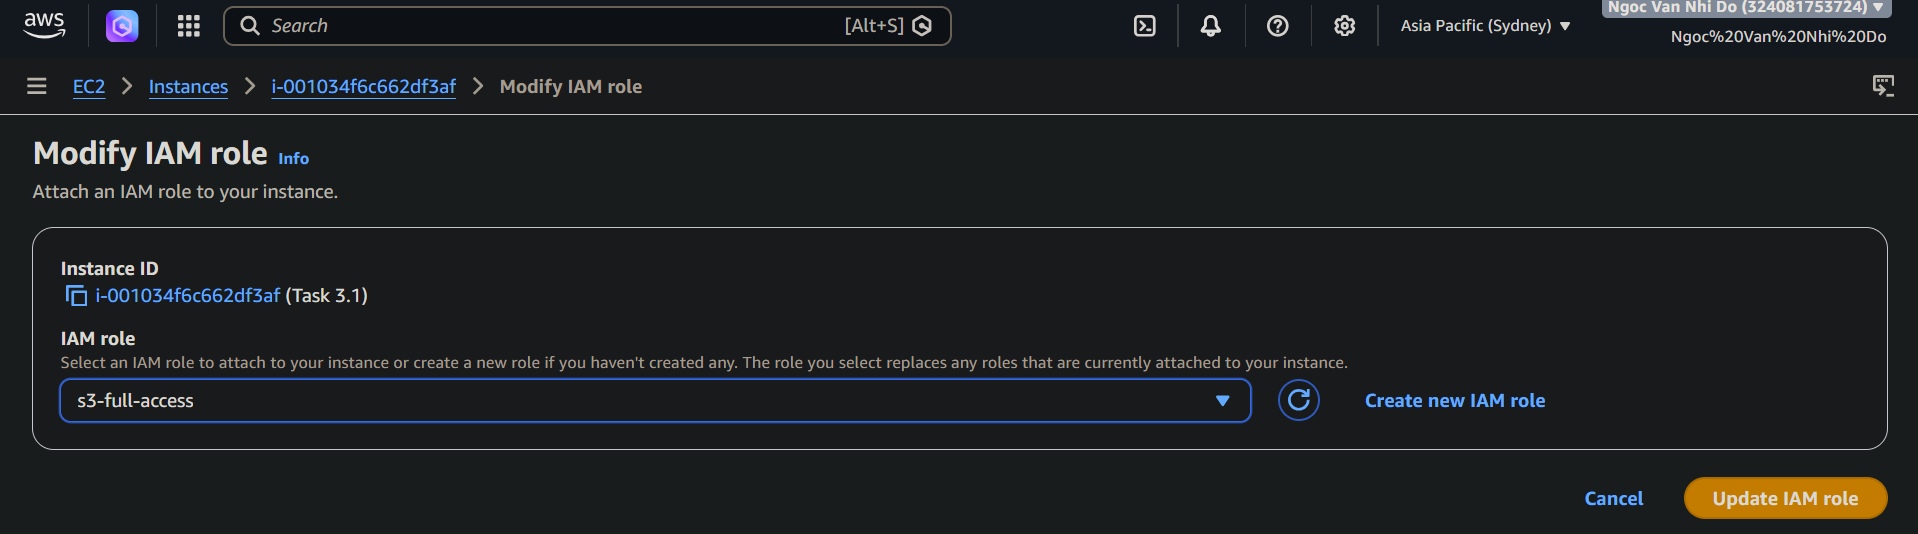
\includegraphics[scale=0.4]{images/2_add_role.jpg}
\vspace{-1em}
\caption{Adding the role to my EC2 instance.}
\end{figure}

I then made a backup of my files by archiving them into a \texttt{.tar} file to avoid having to individually handle hundreds of different files. This archive is then uploaded to the S3 bucket, serving as the backup to my web server.

\begin{figure}[H]
\centering
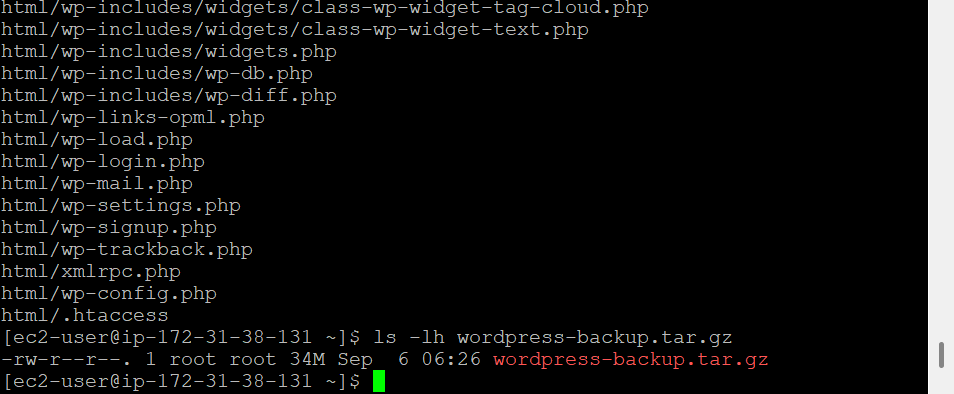
\includegraphics[scale=0.5]{images/2_make_backup.jpg}
\vspace{-1em}
\caption{Creating the backup as a \texttt{.tar} archive.}
\end{figure}

\begin{figure}[H]
\centering
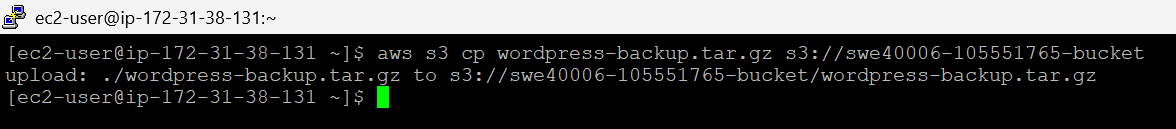
\includegraphics[scale=0.6]{images/2_upload_backup.jpg}
\vspace{-1em}
\caption{Uploading the backup to the S3 bucket.}
\end{figure}

\begin{figure}[H]
\centering
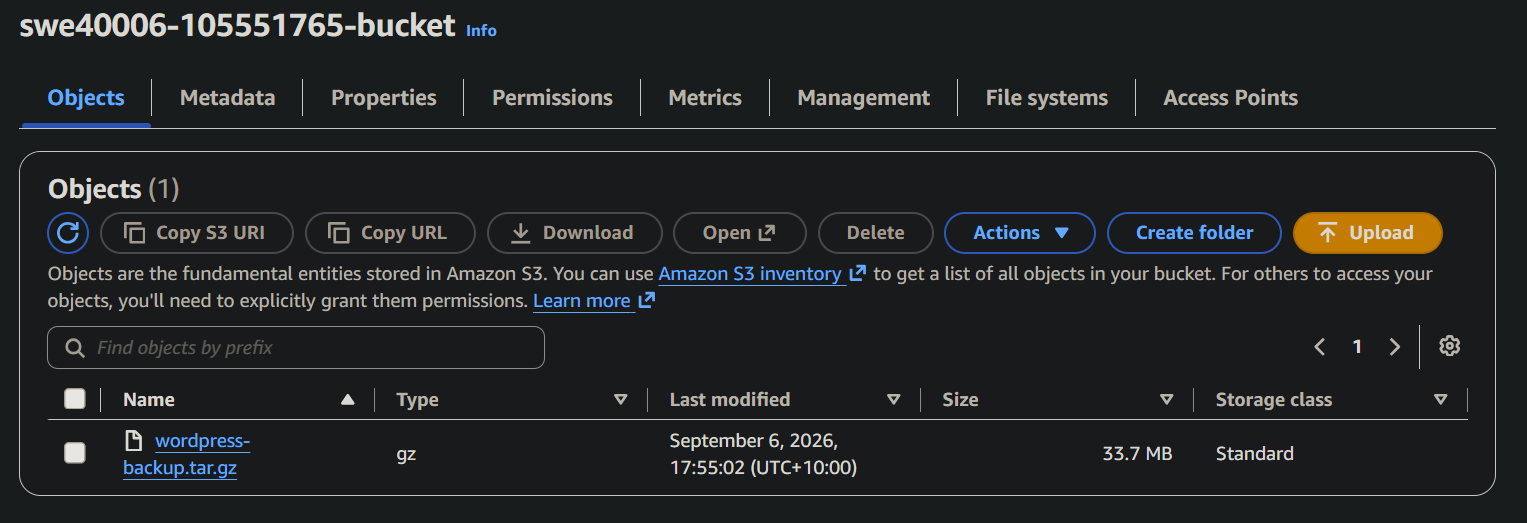
\includegraphics[scale=0.4]{images/2_backup_uploaded.jpg}
\vspace{-1em}
\caption{I could see that the backup has been uploaded using the AWS Console.}
\end{figure}

To demonstrate that I can restore my web server, I first removed all my web application files to simulate a deletion.

\begin{figure}[H]
\centering
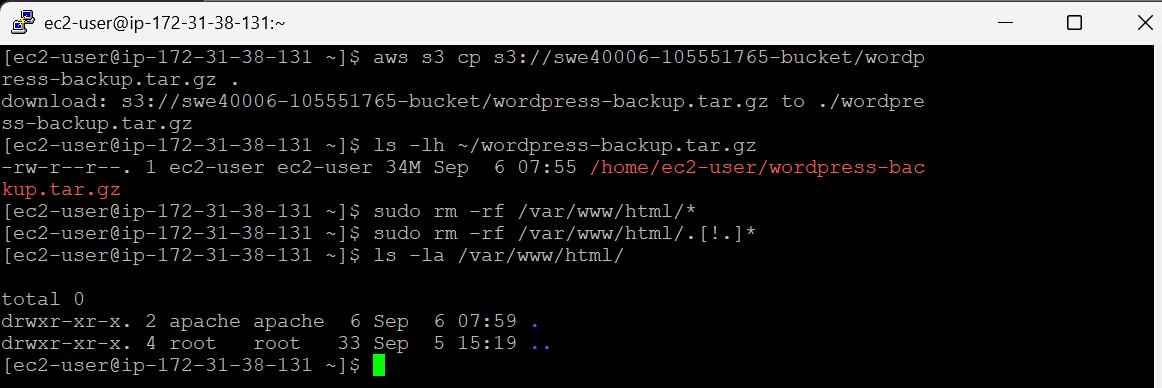
\includegraphics[scale=0.5]{images/2_rm_server.jpg}
\vspace{-1em}
\caption{Removing all web application files on my EC2 instance.}
\end{figure}

Once the files were removed, accessing my website displayed only an "It works!" message rather than the WordPress application, which is the default Apache web server page. This confirmed that the web application had been completely deleted.

\begin{figure}[H]
\centering
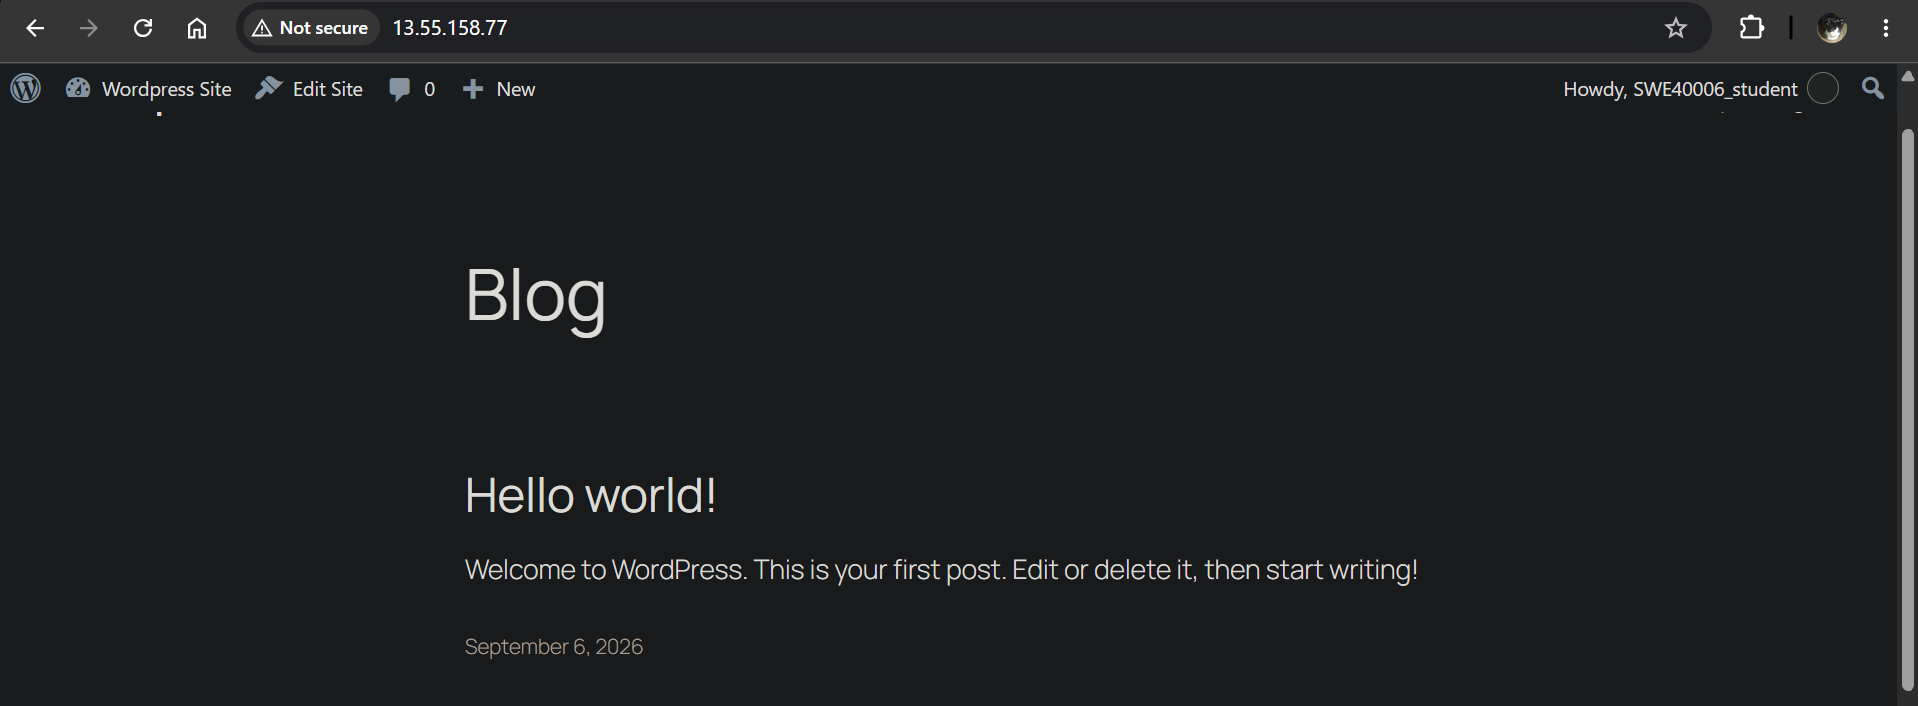
\includegraphics[scale=0.4]{images/2_server_restored.jpg}
\vspace{-1em}
\caption{The WordPress application had been deleted.}
\end{figure}

To restore my deleted web application, I pulled the backup from the S3 bucket and extracted the archived files. The final step was to modify Apache's permissions to be able to read these files and restarting the web server.

\begin{figure}[H]
\centering
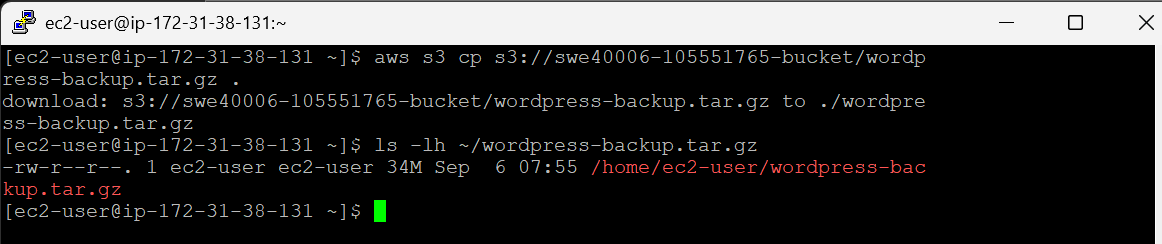
\includegraphics[scale=0.5]{images/2_pull_backup.jpg}
\vspace{-1em}
\caption{Downloading the backup from the S3 bucket.}
\end{figure}

\begin{figure}[H]
\centering
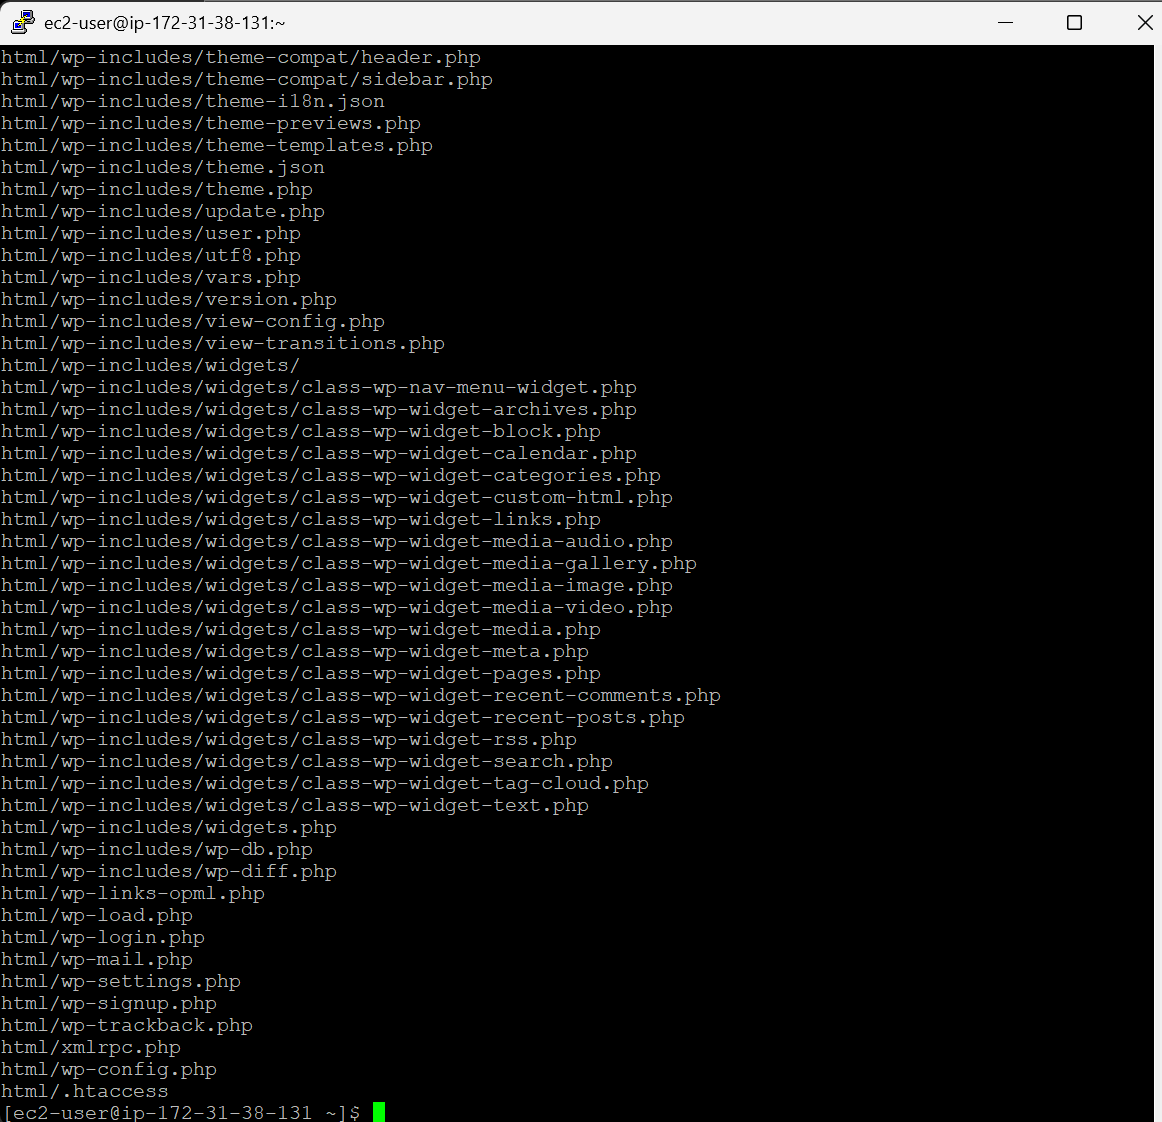
\includegraphics[scale=0.5]{images/2_extract.jpg}
\vspace{-1em}
\caption{Extracting the web application files.}
\end{figure}

\begin{figure}[H]
\centering
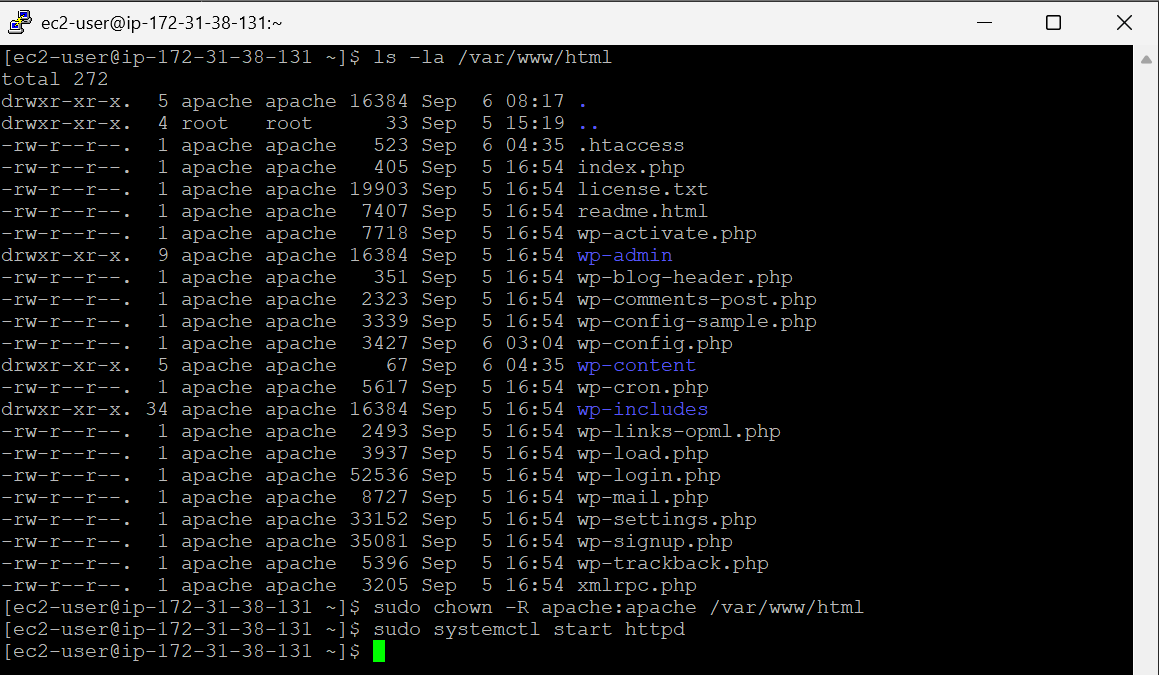
\includegraphics[scale=0.5]{images/2_extracted_files.jpg}
\vspace{-1em}
\caption{Verifying that the application files have been extracted.}
\end{figure}

\begin{figure}[H]
\centering
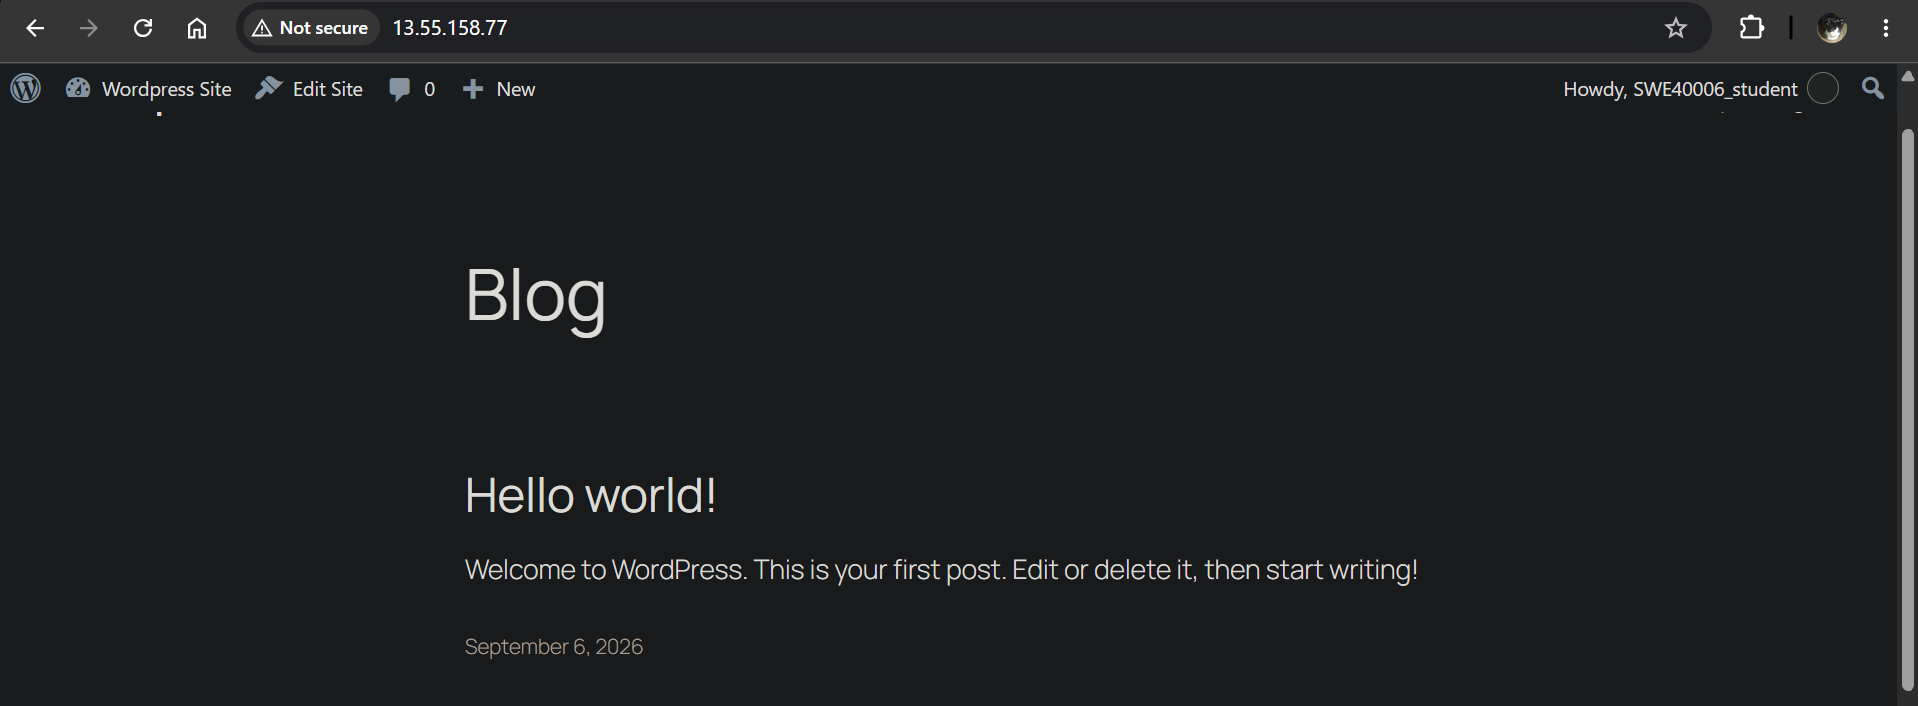
\includegraphics[scale=0.4]{images/2_server_restored.jpg}
\vspace{-1em}
\caption{The web application was successfully restored.}
\end{figure}

\subsection{Task 3.3}

For this task, I created an EC2 Launch Template containing all the necessary configurations to recreate the web server and application on my original EC2 instance. I also provisioned an Application Load Balancer (ALB) across the \texttt{ap-southeast-2a} and \texttt{ap-southeast-2b} availability zones to route public HTTP/HTTPS traffic. The load balancer will route traffic to a target group managed by an Auto Scaling Group (ASG). The ASG uses the Launch Template to configure EC2 instances and maintains the desired number of instances, launching new instances in the event of instance failures.

\subsubsection{Creating the Launch Template}

A new launch template (\texttt{task-3-3-template}) is created and configured with the Amazon Linux AMI, the \texttt{t3.micro} instance type, and the security group \texttt{task-3.1-sg} that was used for the original EC2 instance.

\begin{figure}[H]
\centering
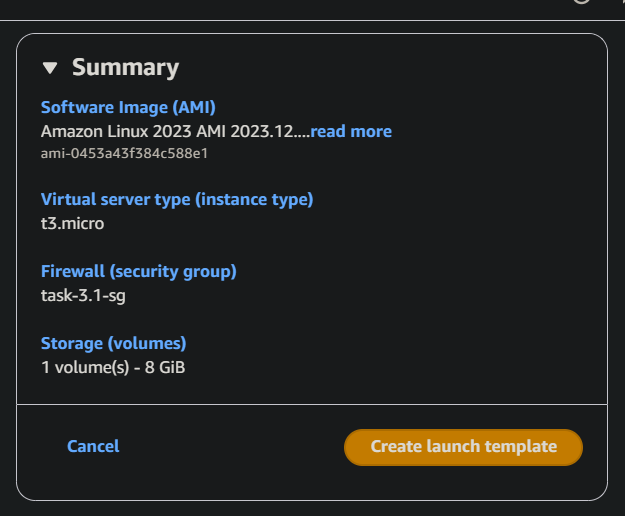
\includegraphics[scale=0.6]{images/3_create_template.jpg}
\vspace{-1em}
\caption{Summary of the launch template's configurations.}
\end{figure}

Configuring the user data for this template is especially important, as it is the startup script that runs when the instance launches, ensuring that everything necessary is correctly intsalled and configured to serve our web application. The script below updates the OS, installs the web server, PHP, and AWS CLI, starts Apache and PHP\_FPM, creates the WordPress web directory, downloads the backup that I created earlier from S3, extracts the files, sets file permissions, and restarts the web server.

\begin{figure}[H]
\centering
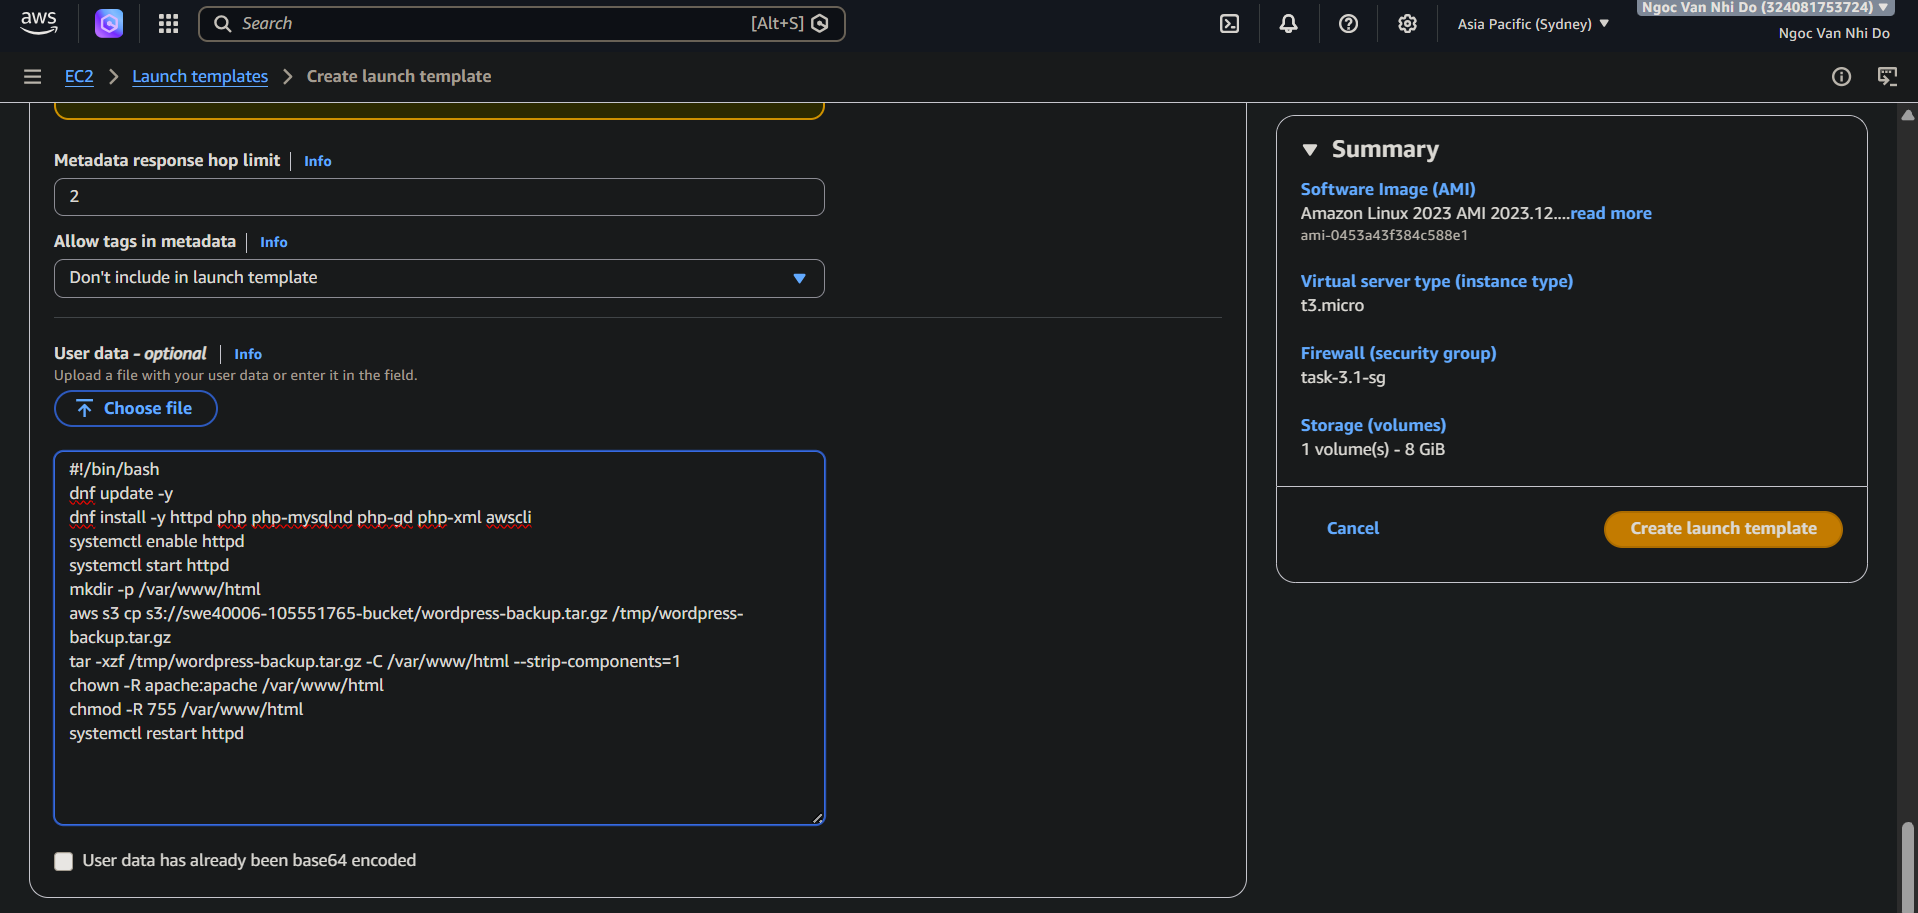
\includegraphics[scale=0.4]{images/3_user_data.jpg}
\vspace{-1em}
\caption{The template's user data script.}
\end{figure}

\subsubsection{Creating the Application Load Balancer (ALB)}

Before creating the ALB, I had to set up a new security group for it. The idea is to put the ALB in front my my application instance and make the instances private from the public internet. The ALB will handle incoming HTTP/HTTPS traffic from users on the internet, then distribute these requests across the application instances.

The ALB's security group will allow inbound HTTP/HTTPS traffic from anywhere.

\begin{figure}[H]
\centering
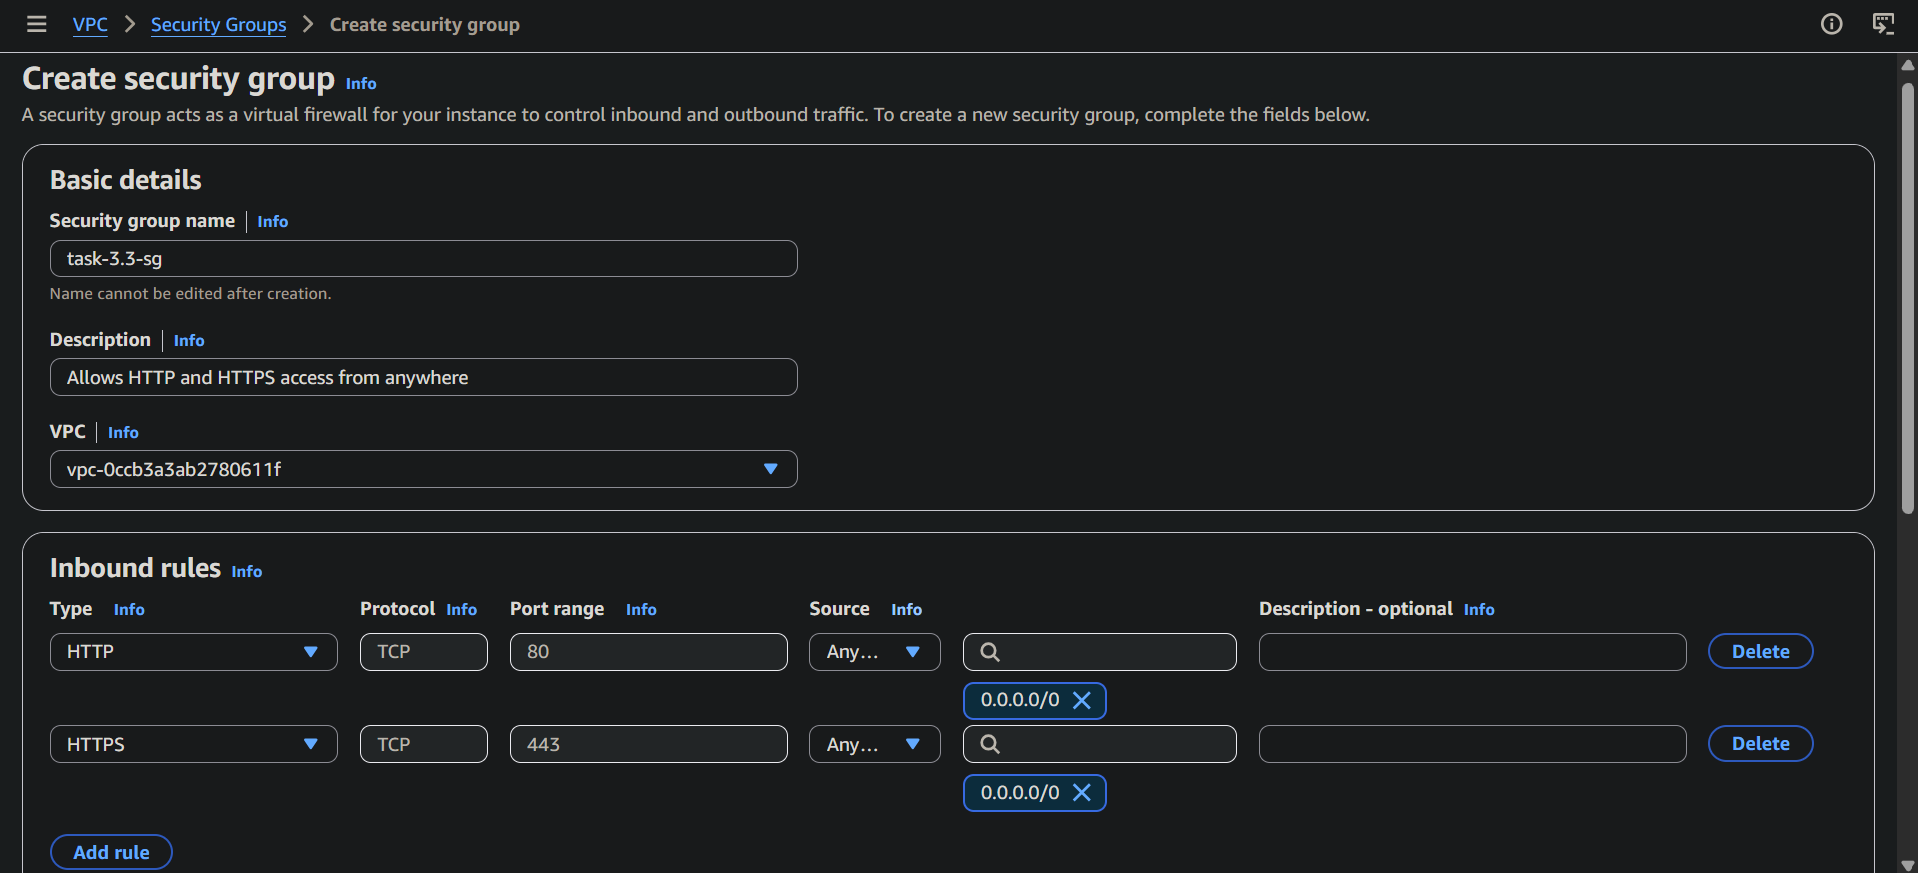
\includegraphics[scale=0.4]{images/3_create_sg.jpg}
\vspace{-1em}
\caption{Creating a new security group for the ALB.}
\end{figure}

The inbound rules for the security group that was used for the original EC2 instance were also changed to only receive HTTP traffic from the ALB's security group. This also implies that the web application hosted on the first EC2 instance is no longer publicly accessible.

\begin{figure}[H]
\centering
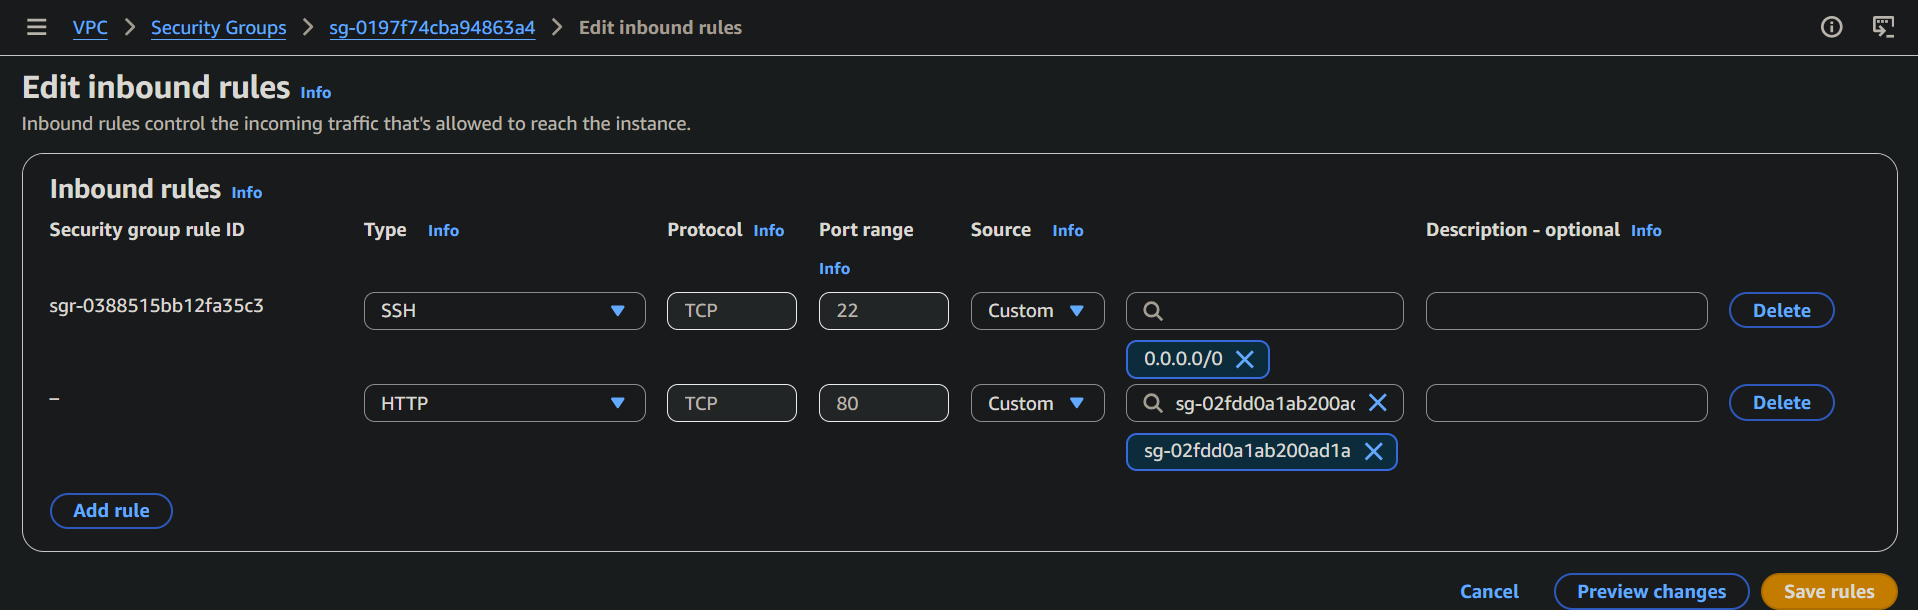
\includegraphics[scale=0.4]{images/3_edit_sg.jpg}
\vspace{-1em}
\caption{Configuring the rules for the application instances' security group to no longer allow HTTP traffic from the internet.}
\end{figure}

I then created an ALB (\texttt{task-3-3-alb}) spanning the availability zones \texttt{ap-southeast-2a} and \texttt{ap-southeast-2b}, configured with the security group \texttt{task-3.3-sg} that was just created above.

\begin{figure}[H]
\centering
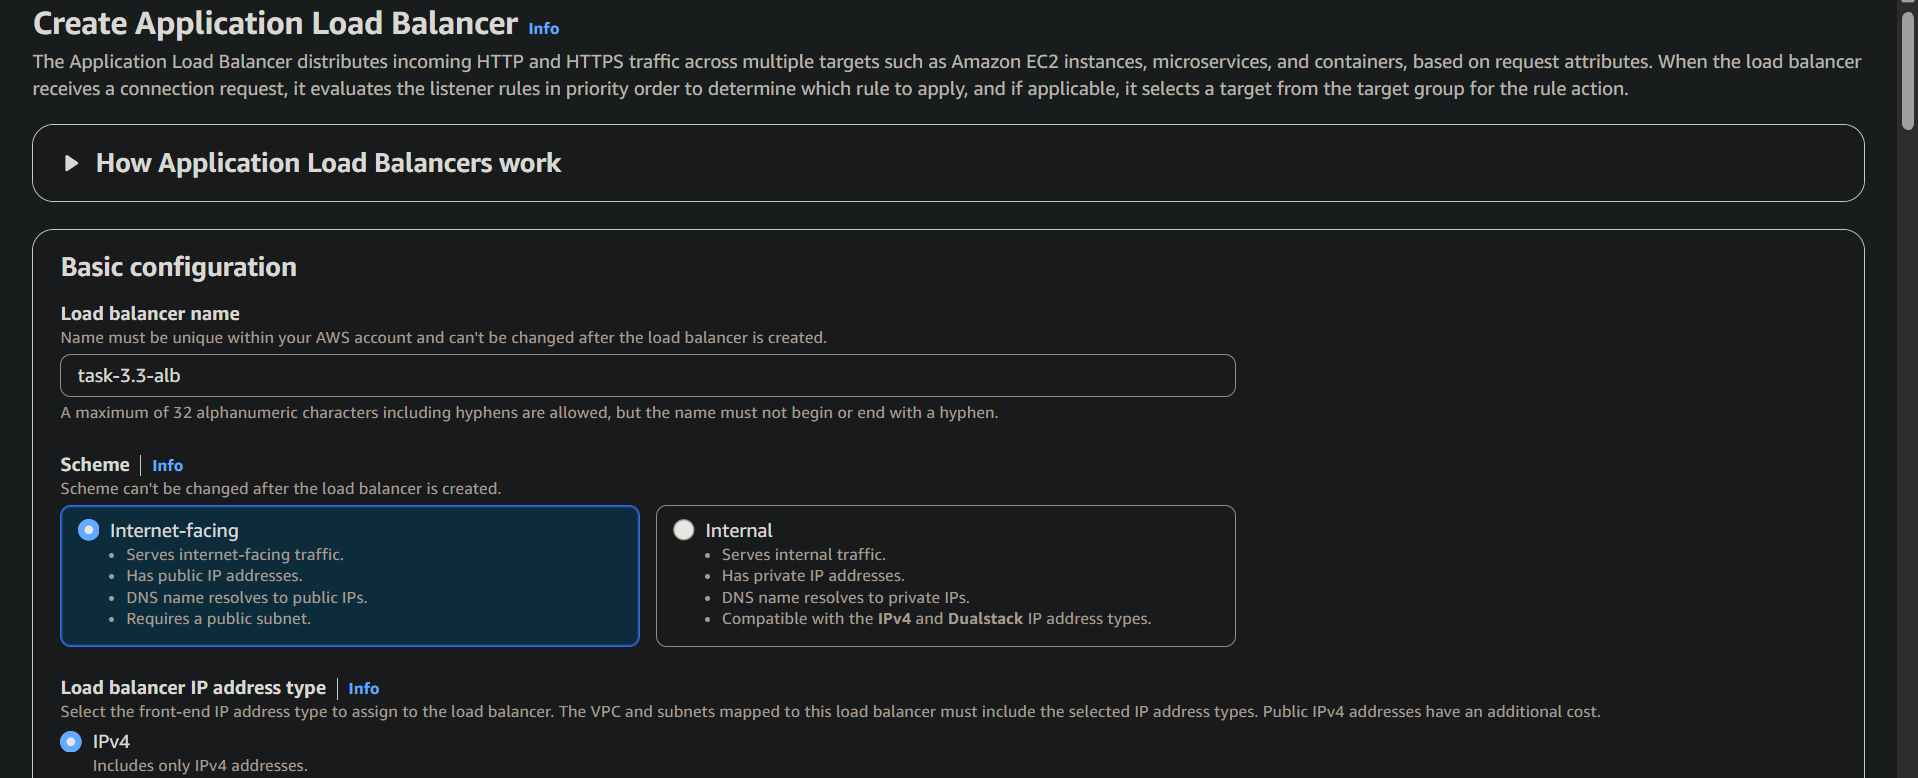
\includegraphics[scale=0.4]{images/3_create_alb.jpg}
\vspace{-1em}
\caption{Creating a new ALB with the name \texttt{task-3-3-alb}.}
\end{figure}

\begin{figure}[H]
\centering
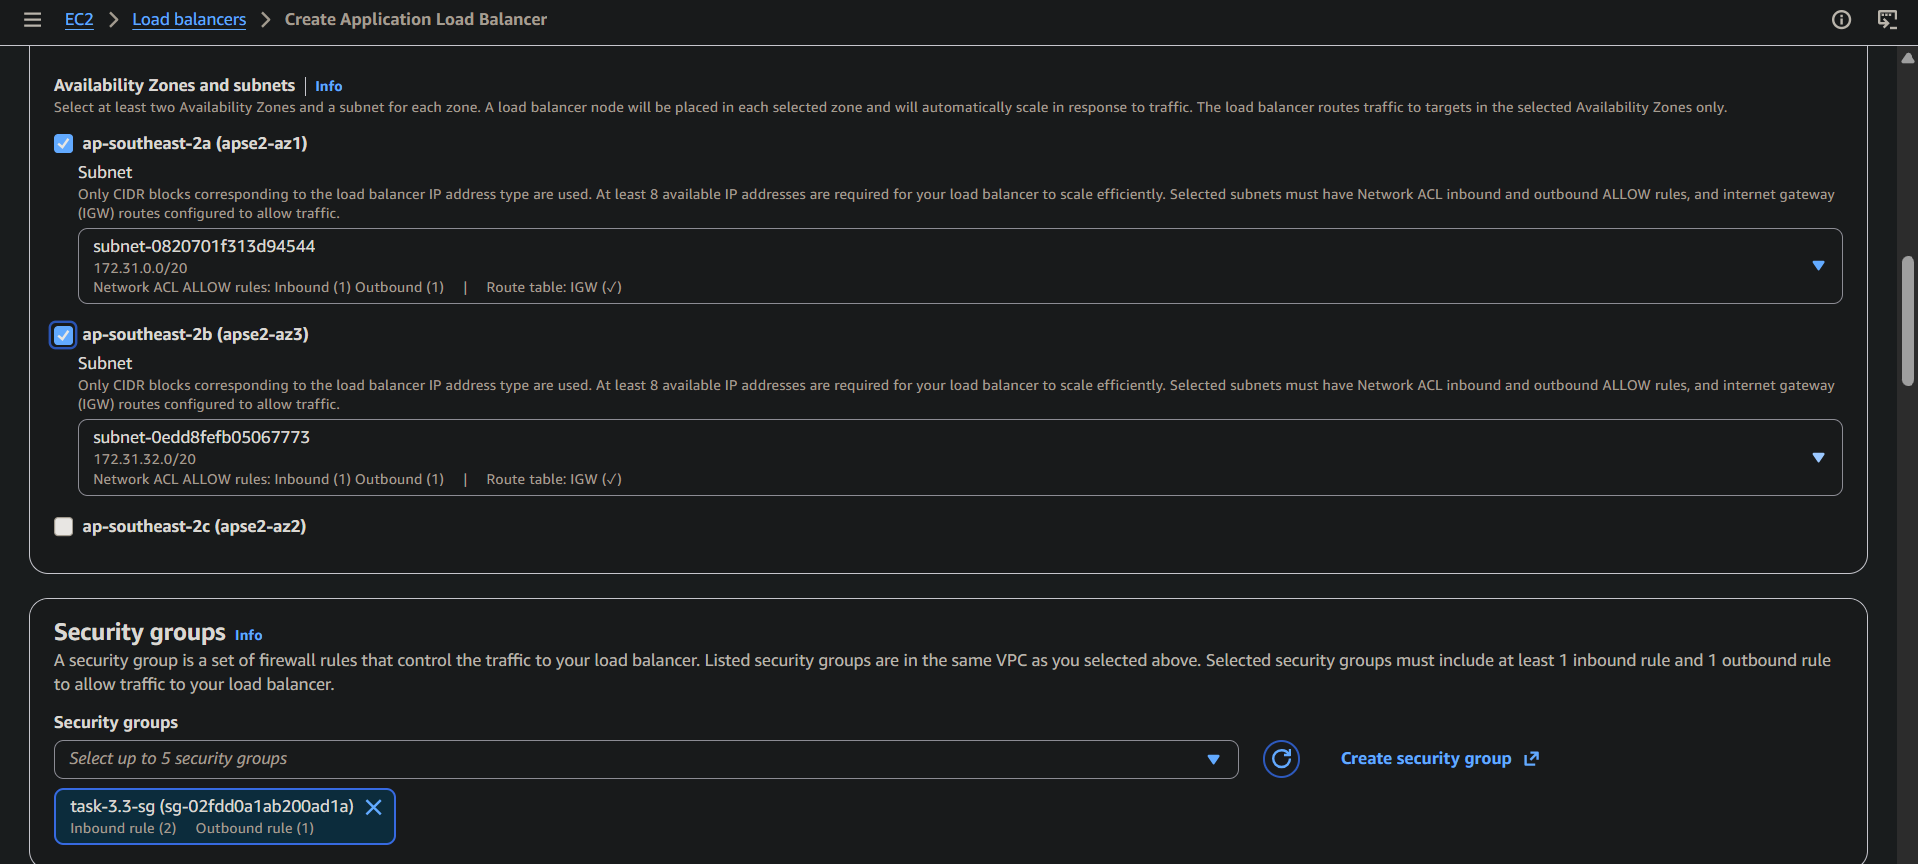
\includegraphics[scale=0.4]{images/3_alb_network.jpg}
\vspace{-1em}
\caption{Configuring the ALB's availability zones and security group.}
\end{figure}

I also created a new target group that would receive traffic from the ALB. A health check was configured on port 80 to verify that the instances would be running and responding correctly. The target group was then attached to the ALB, allowing the ALB to forward incoming traffic to healthy instances.

\begin{figure}[H]
\centering
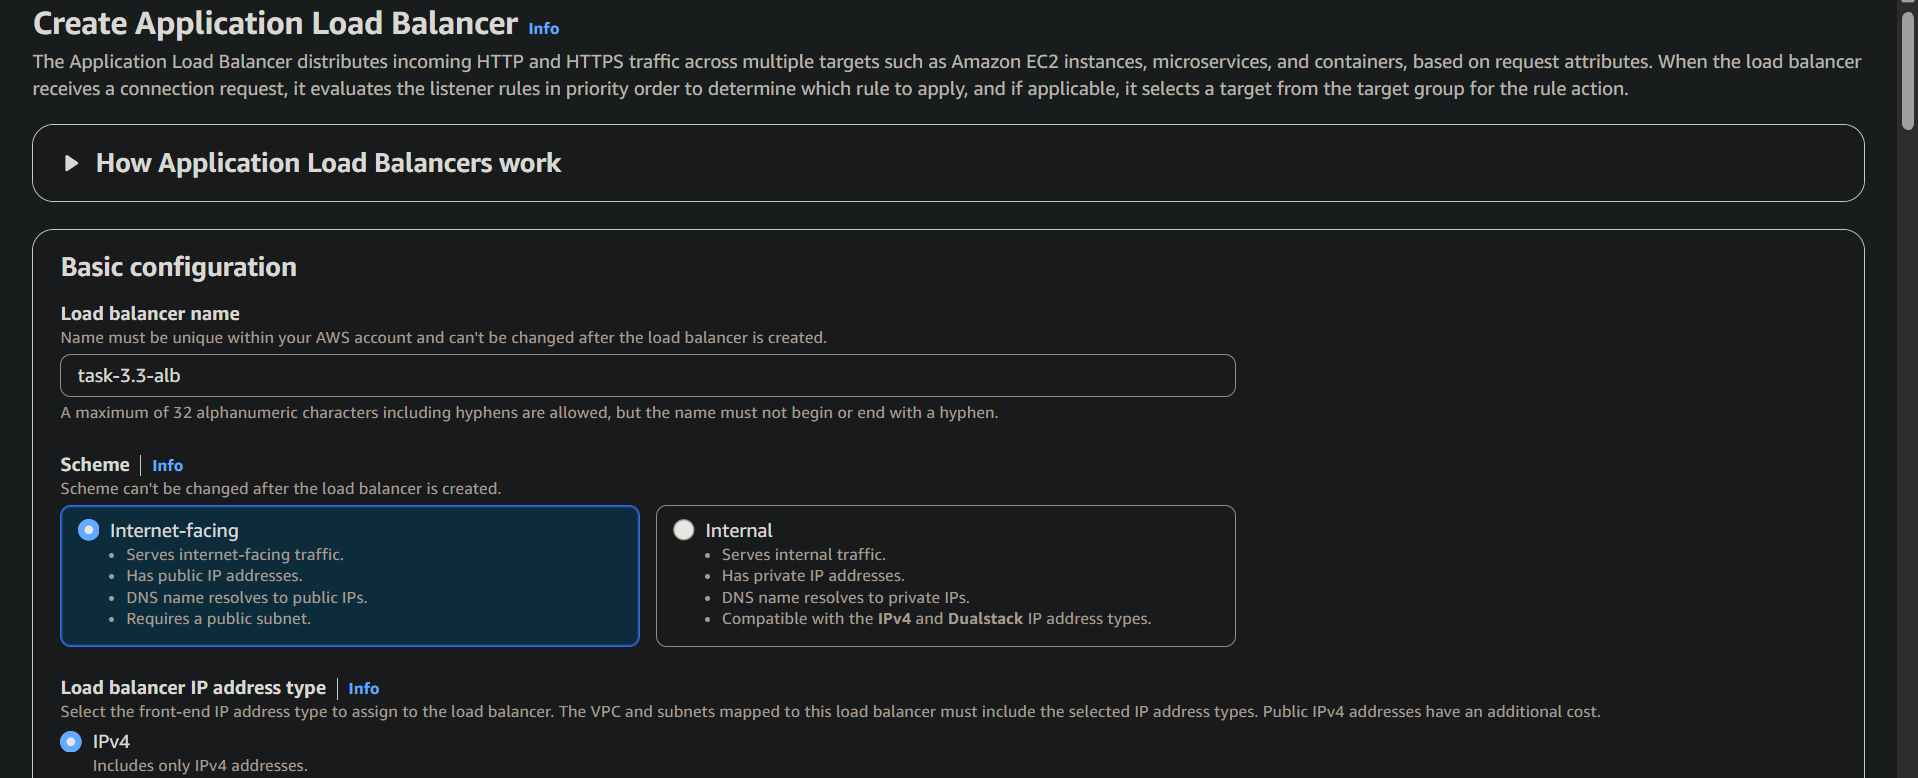
\includegraphics[scale=0.4]{images/3_create_alb.jpg}
\vspace{-1em}
\caption{Creating a new target group \texttt{task-3-3-tg}. The target group is not registered with any instances for now.}
\end{figure}

\begin{figure}[H]
\centering
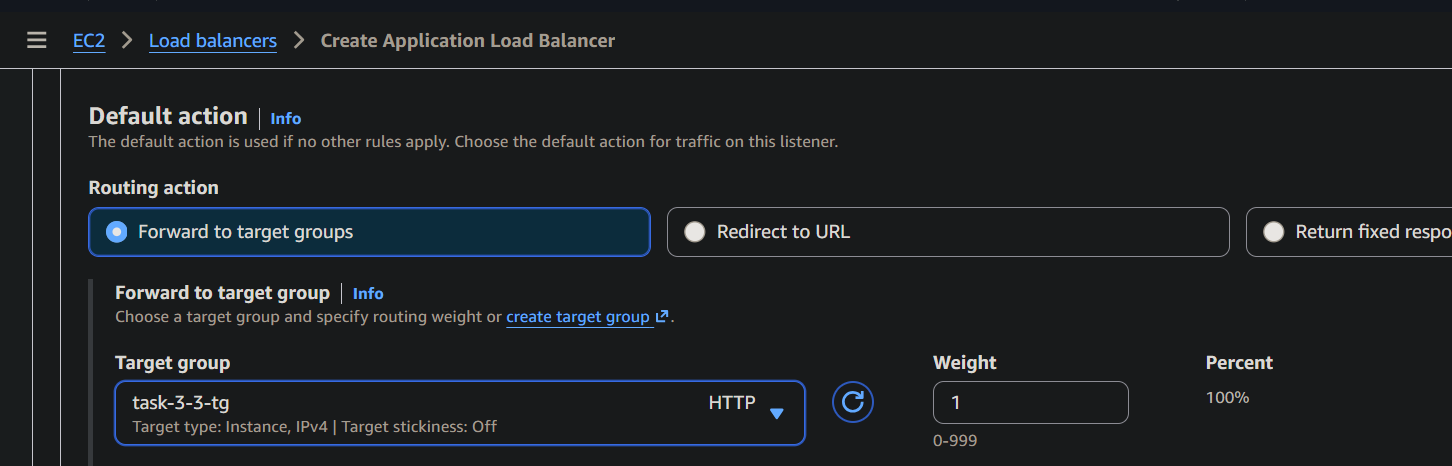
\includegraphics[scale=0.4]{images/3_alb_tg.jpg}
\vspace{-1em}
\caption{Attaching \texttt{task-3-3-tg} to the ALB.}
\end{figure}

\subsubsection{Creating the Auto Scaling Group (ASG)}

I then created a new ASG with the following configurations:

\begin{itemize}[nosep]
    \item Name: \texttt{task-3-3-asg}
    \item Launch template: \texttt{task-3-3-template}
    \item Availability Zones: \texttt{ap-southeast-2a} and \texttt{ap-southeast-2b} (matching the ALB's availability zones)
    \item Load balancer: \texttt{task-3-3-alb}
    \item Target group: \texttt{task-3-3-tg}
    \item Desired capacity: 2
    \item Minimum capacity: 2
    \item Maximum capacity: 4
\end{itemize}

\begin{figure}[H]
\centering
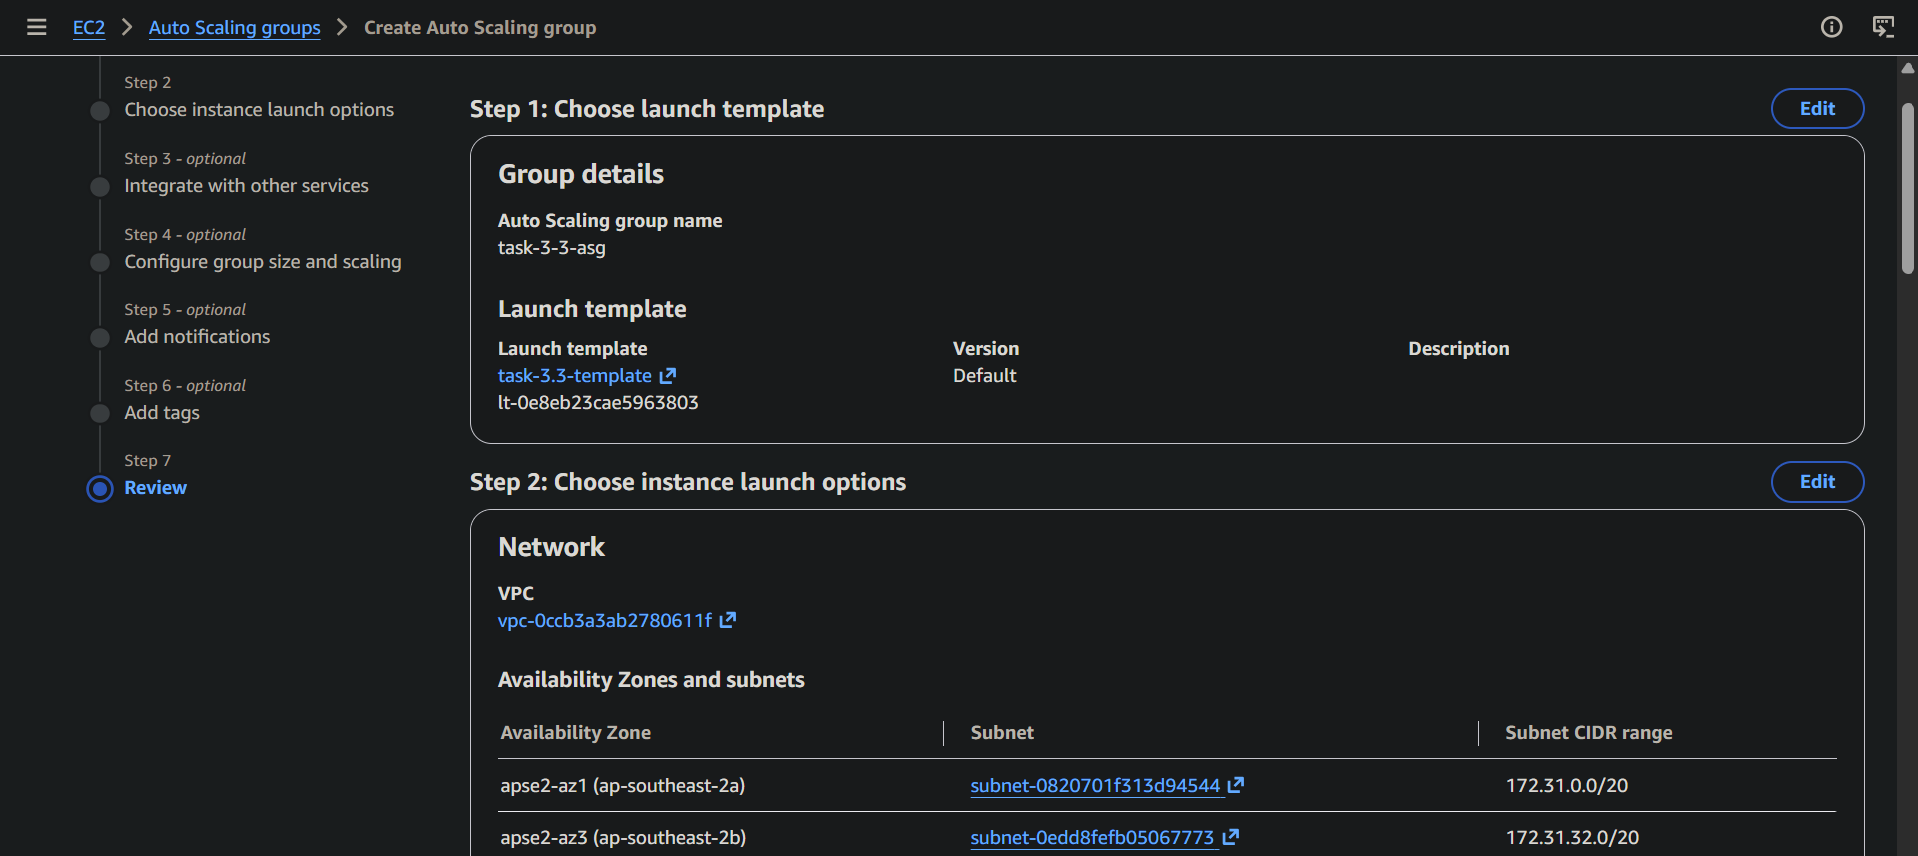
\includegraphics[scale=0.4]{images/3_create_asg.jpg}
\vspace{-1em}
\end{figure}

\begin{figure}[H]
\centering
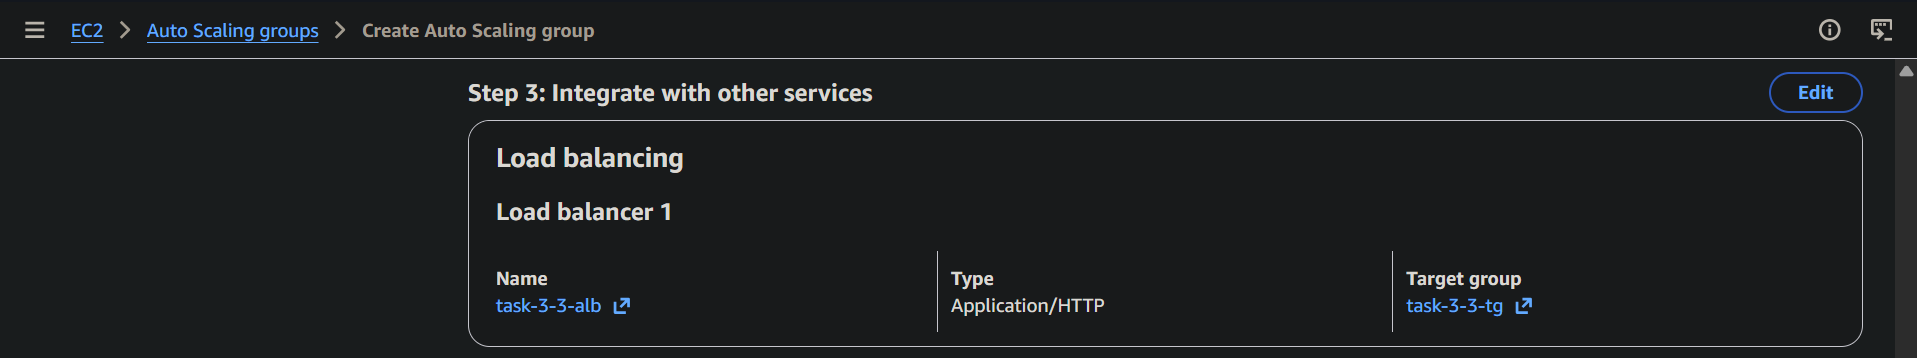
\includegraphics[scale=0.4]{images/3_asg_alb.jpg}
\vspace{-1em}
\end{figure}

\begin{figure}[H]
\centering
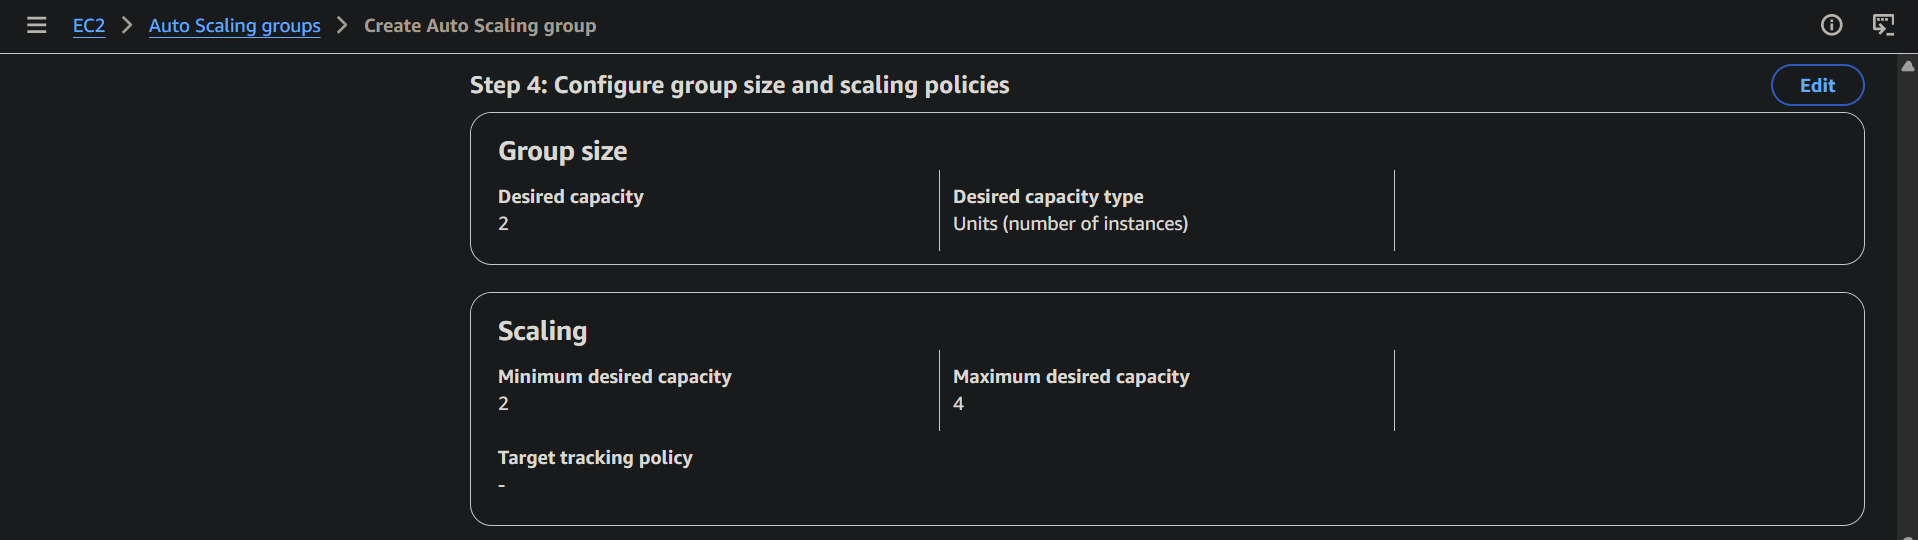
\includegraphics[scale=0.4]{images/3_config_capacity.jpg}
\vspace{-1em}
\caption{A summary of ASG's configurations.}
\end{figure}

\subsubsection{Verification}

Once everything had been set up and configured, I noticed that the health checks for my instances were returning an "Unhealthy" status. I initially suspected that the issue was related to networking for traffic being unable to reach the instances correctly. I began investigating the VPC configuration, security groups, inbound and outbound security rules, and the availability zones to ensure that everything was correctly configured. After confirming that these settings were correct, I decided to SSH into one of the failing instances to further troubleshoot this issue.

\begin{figure}[H]
\centering
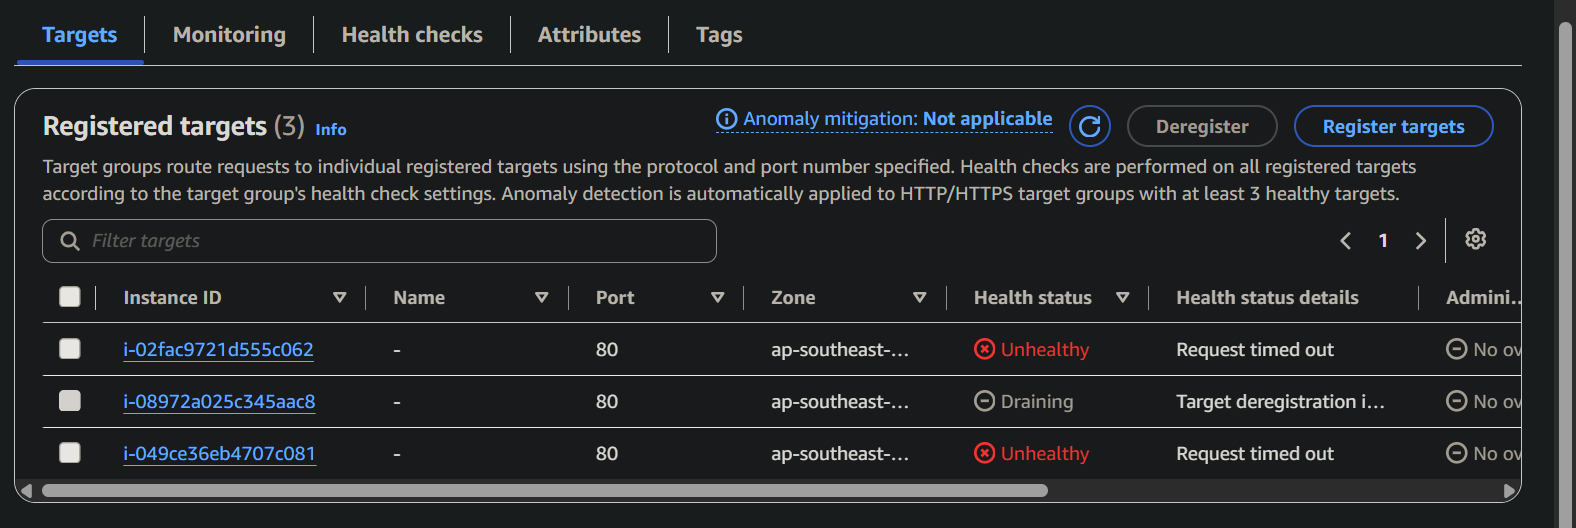
\includegraphics[scale=0.5]{images/3_unhealthy.jpg}
\vspace{-1em}
\caption{Health checks were returning an "Unhealthy" status, causing the ASG to deregister failing instances and launch new ones to replace them.}
\end{figure}

I investigated a wide range of potential issues, checking installed dependencies and making sure they were running, verifying that the web application files were properly installed into the correct directory, or that the database configurations contained the correct information. Testing showed that Apache and PHP-FPM were running correctly and that PHP scripts could execute successfully. The WordPress installation was also correctly restored from the S3 backup, including the \texttt{wp-config.php} file, which pointed to the RDS database. The root cause was an incorrect RDS security group configuration that prevented the EC2 intsances from connecting to the database on port 3306. When the ALB requests \texttt{/}, WordPress tried to connect to the database and hung waiting for the database connection, which made Apache eventually time out.

\begin{figure}[H]
\centering
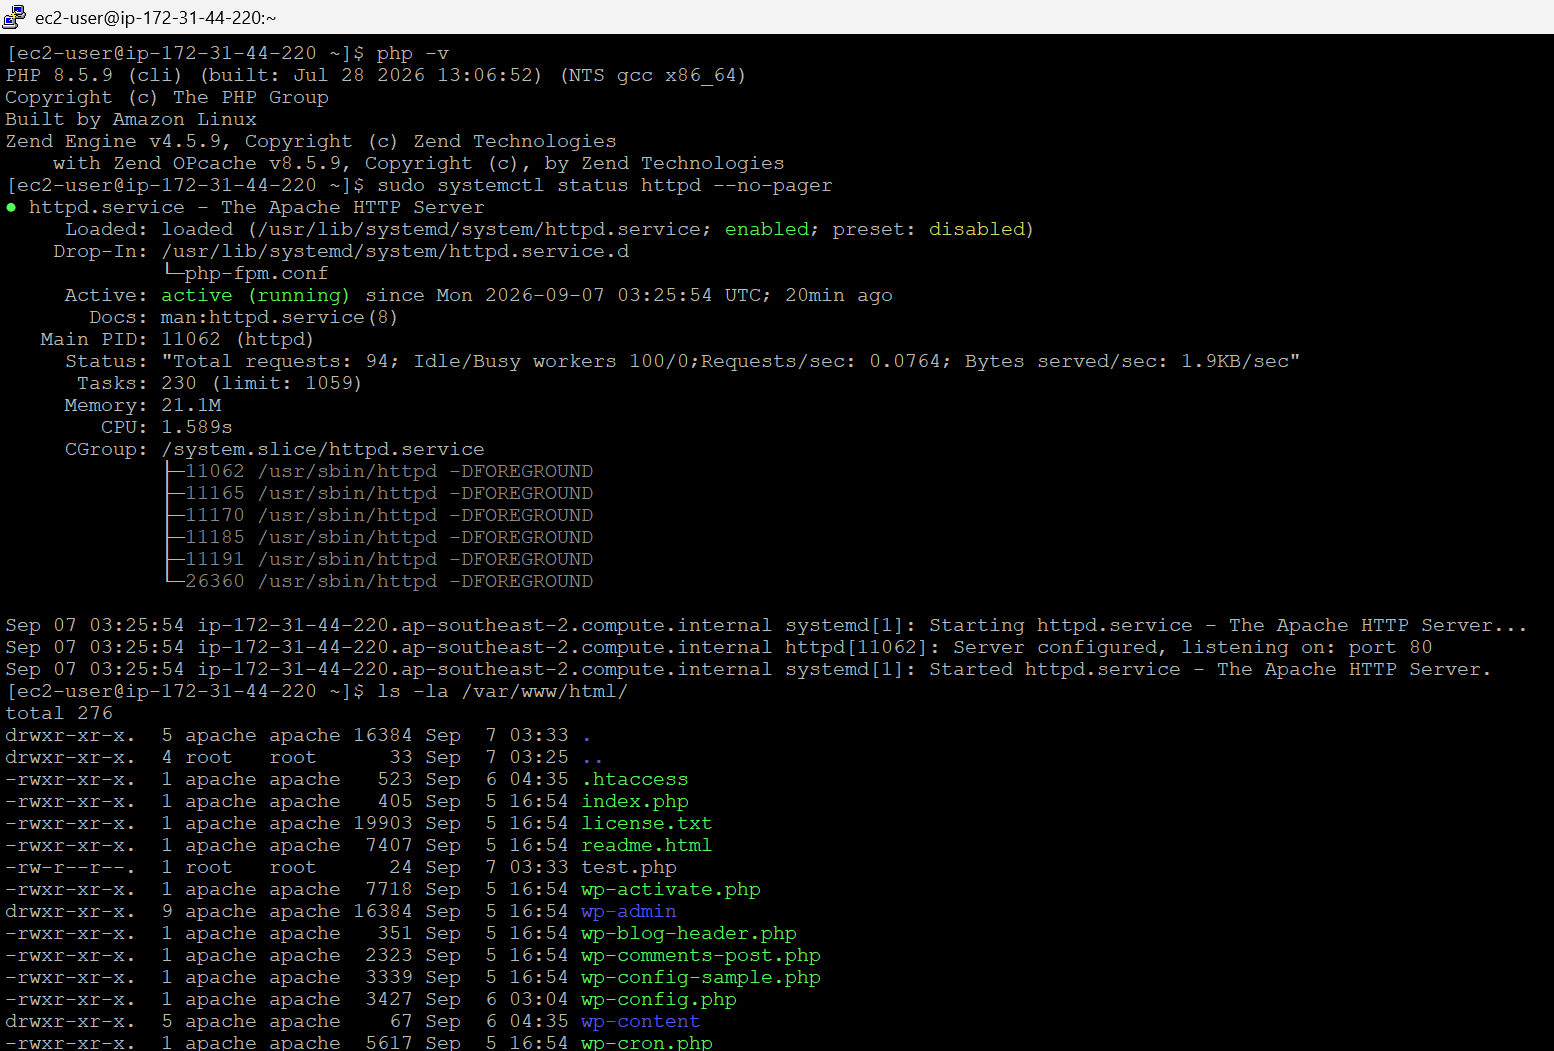
\includegraphics[scale=0.4]{images/3_debug_files.jpg}
\vspace{-1em}
\caption{Checking that the application files were restored correctly.}
\end{figure}

\begin{figure}[H]
\centering
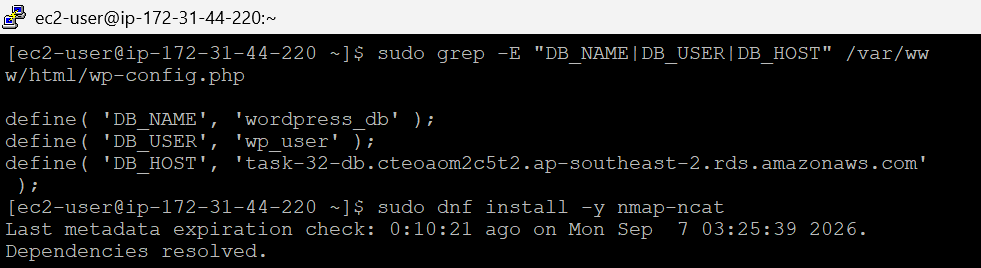
\includegraphics[scale=0.6]{images/3_debug_configs.jpg}
\vspace{-1em}
\caption{Verifying that the database configurations are correct.}
\end{figure}

\begin{figure}[H]
\centering
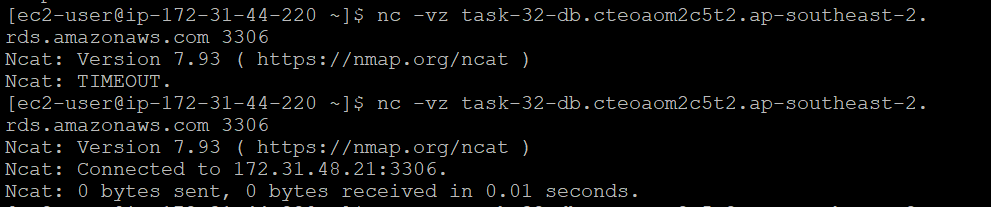
\includegraphics[scale=0.6]{images/3_debug_db.jpg}
\vspace{-1em}
\caption{An initial attempt to connect to the RDS database timed out. The second attempt showed a successful connection after the problem had been fixed.}
\end{figure}

The RDS instance's security group was allowing MySQL traffic on port 3306 from another security group that was not configured with the applications instances. This was fixed by adding the correct inbound security rule.

\begin{figure}[H]
\centering
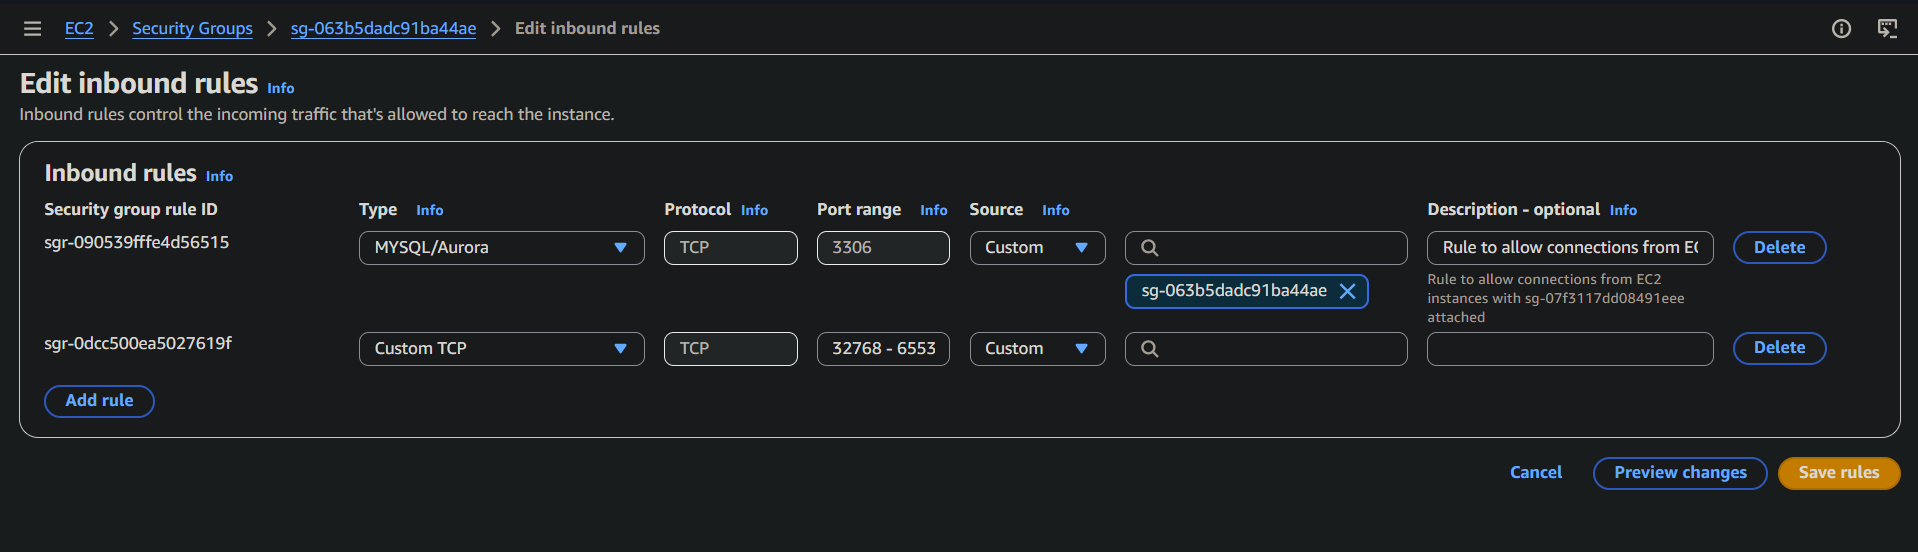
\includegraphics[scale=0.4]{images/3_db_sg.jpg}
\vspace{-1em}
\end{figure}

\begin{figure}[H]
\centering
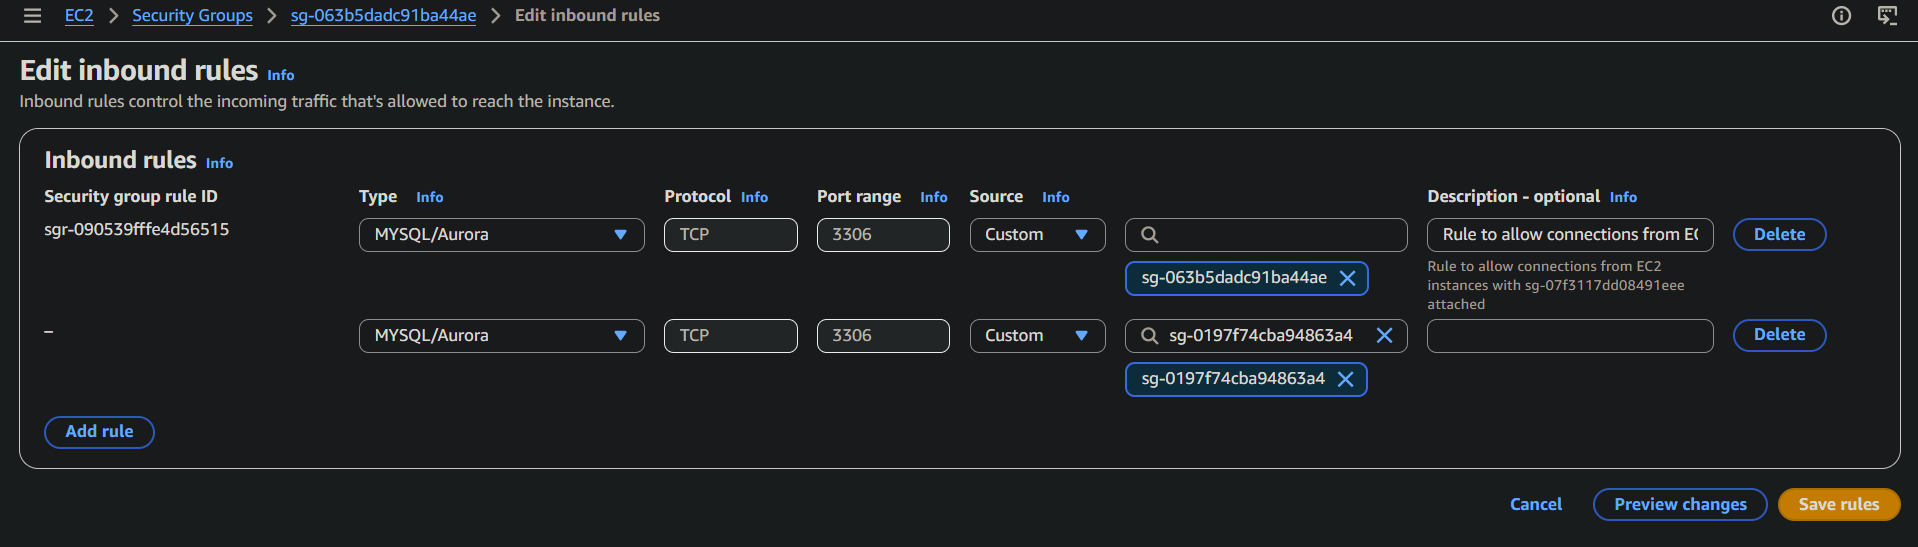
\includegraphics[scale=0.4]{images/3_fix_sg.jpg}
\vspace{-1em}
\caption{Adding the correct security rule so that the instances could connect to the RDS database.}
\end{figure}

The health checks now return a "Healthy" status for both instances, confirming that the ALB can communicate with them correctly. The application can be accessed through the ALB's DNS name at \url{http://task-3-3-alb-2099008439.ap-southeast-2.elb.amazonaws.com/}.

\begin{figure}[H]
\centering
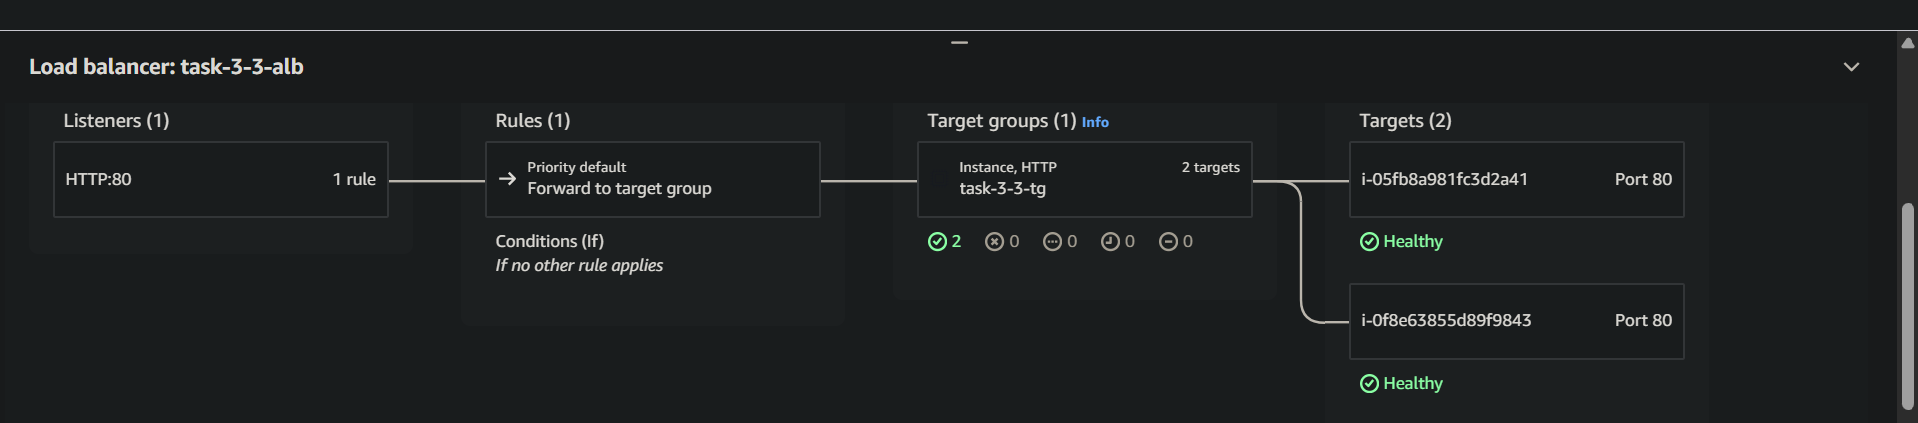
\includegraphics[scale=0.4]{images/3_fixed.jpg}
\vspace{-1em}
\caption{Health checks return "Healthy" status.}
\end{figure}

\begin{figure}[H]
\centering
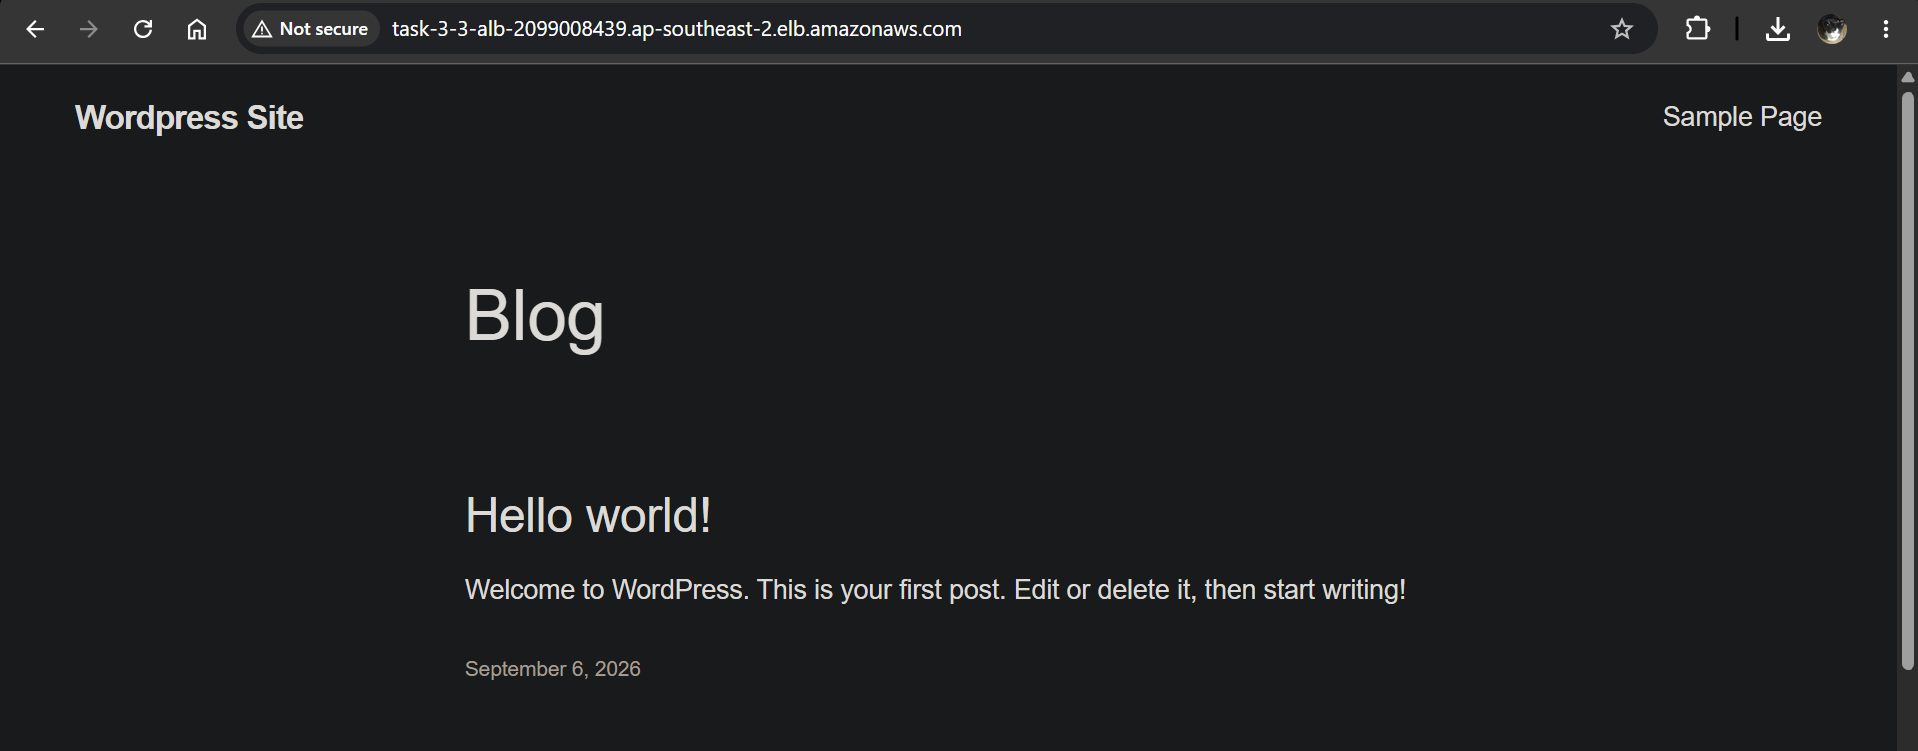
\includegraphics[scale=0.4]{images/3_live_site.jpg}
\vspace{-1em}
\caption{The application is running live and can be accessed through the ALB.}
\end{figure}

\subsection{Task 3.4}

For task 3.4, I configured a CloudWatch alarm for the Auto Scaling Group to monitor CPU utilisation and trigger when it exceeds 70\% over a 5-minute period. An Amazon SNS topic was configured to send an email notification to my student email address when the alarm is triggered. I also enabled AWS Systems Manager (SSM) Session Manager for the EC2 instances, allowing secure terminal access through the AWS Console without requiring public SSH access or open port 22.

\subsubsection{CloudWatch Monitoring and Alarm}

Before creating the alarm, I set up an SNS topic called \texttt{task-3-4-topic}. The CloudWatch alarm uses this topic as the destination to send its notifications, publishing a message when the alarm is triggered by a pre-defined metric. Subscribers to the SNS topic can then receive those notifications.

\begin{figure}[H]
\centering
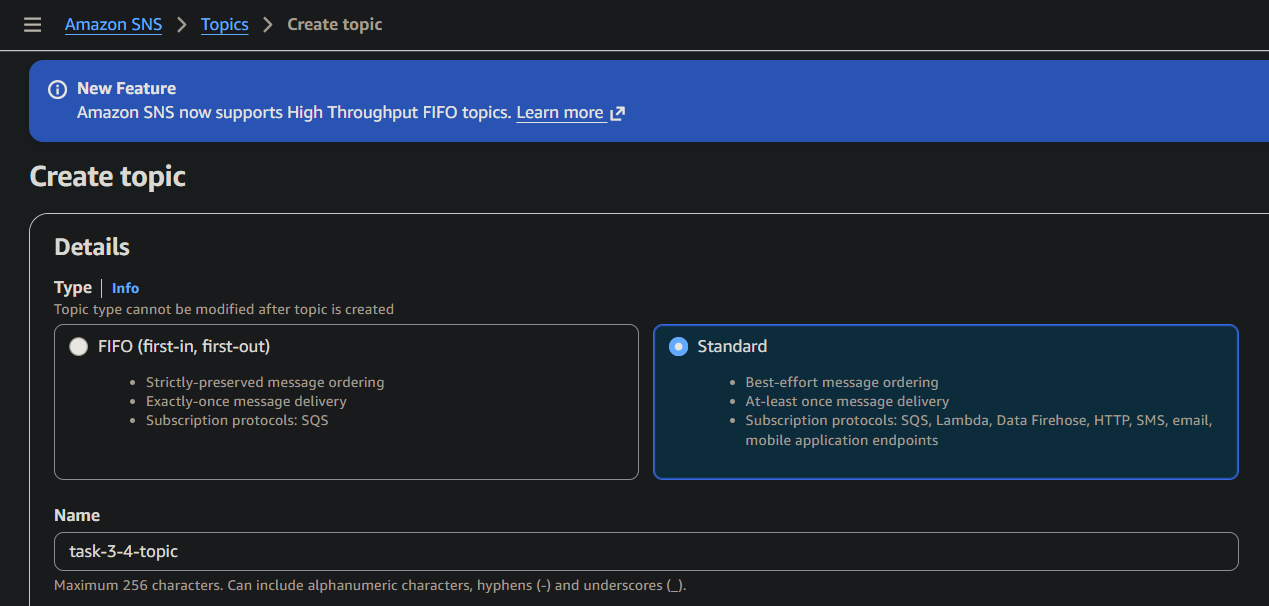
\includegraphics[scale=0.5]{images/4_create_topic.jpg}
\vspace{-1em}
\caption{Creating a new SNS topic \texttt{task-3-4-topic}.}
\end{figure}

I then subscribed to this topic so that I could receive an email whenever the CloudWatch alarm gets triggered.

\begin{figure}[H]
\centering
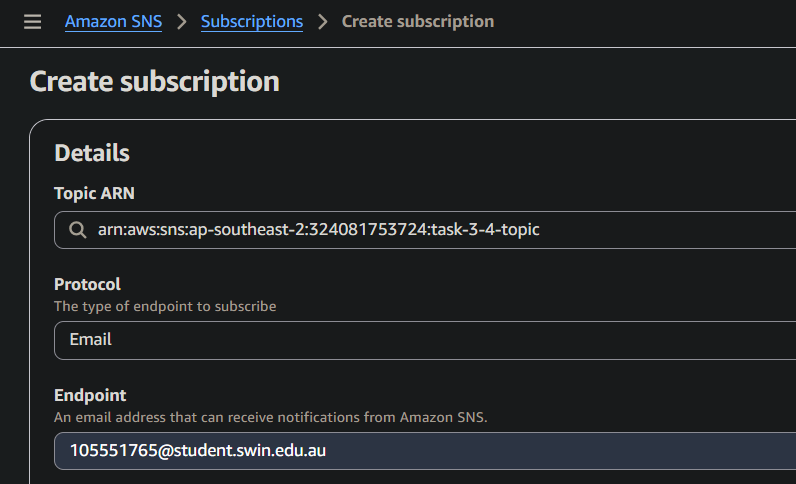
\includegraphics[scale=0.5]{images/4_create_subscription.jpg}
\vspace{-1em}
\caption{Subscribing to the SNS topic.}
\end{figure}

\begin{figure}[H]
\centering
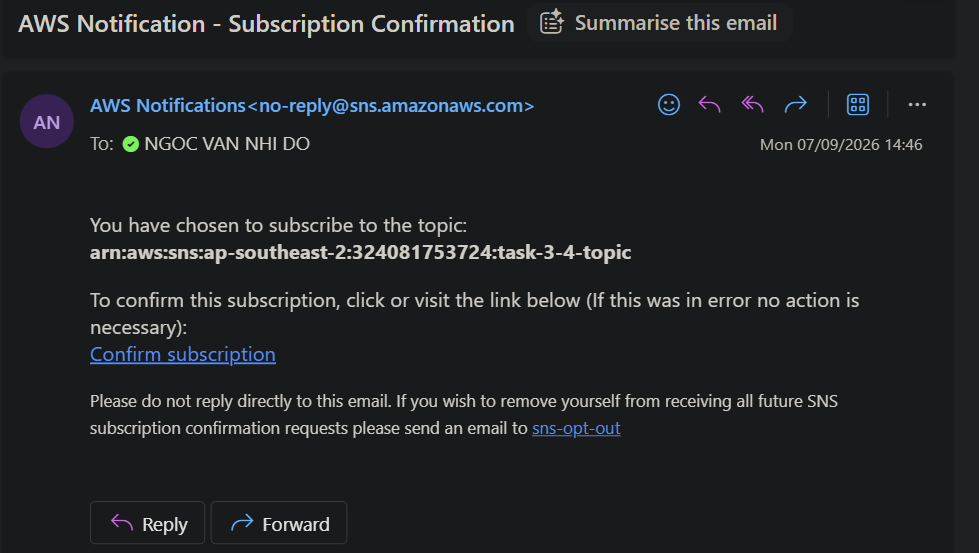
\includegraphics[scale=0.4]{images/4_verify_subscription.jpg}
\vspace{-1em}
\caption{An email is sent to my student email address to verify the subscription.}
\end{figure}

\begin{figure}[H]
\centering
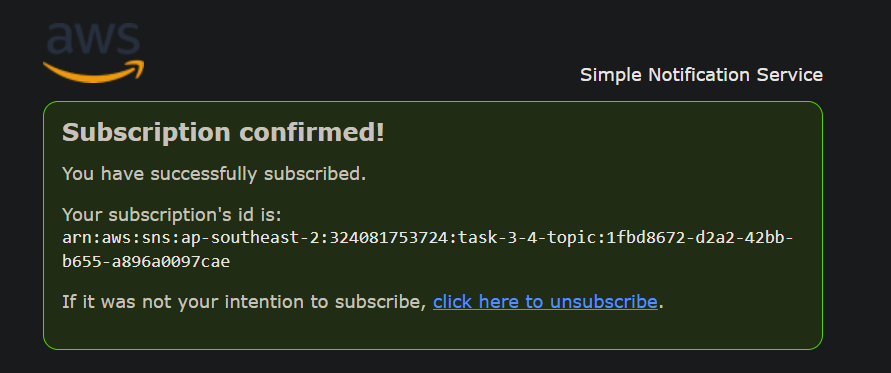
\includegraphics[scale=0.5]{images/4_subscription_verified.jpg}
\vspace{-1em}
\caption{My subscription is verified.}
\end{figure}

The next step was creating the CloudWatch alarm itself. I set up an alarm on the \texttt{CPUUtilization} metric for my ASG \texttt{task-3-3} rather on the individual EC2 instances. I also set the threshold for the alarm to "greater than 70", meaning that the alarm is triggered with CPU utilisation exceeds 70\% for over 5 minutes.

\begin{figure}[H]
\centering
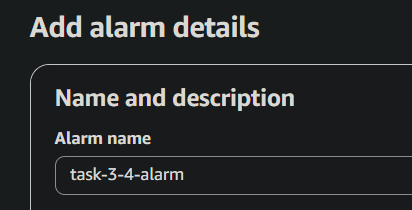
\includegraphics[scale=0.6]{images/4_create_alarm.jpg}
\vspace{-1em}
\caption{Creating a new CloudWatch alarm \texttt{task-3-4-alarm}.}
\end{figure}

\begin{figure}[H]
\centering
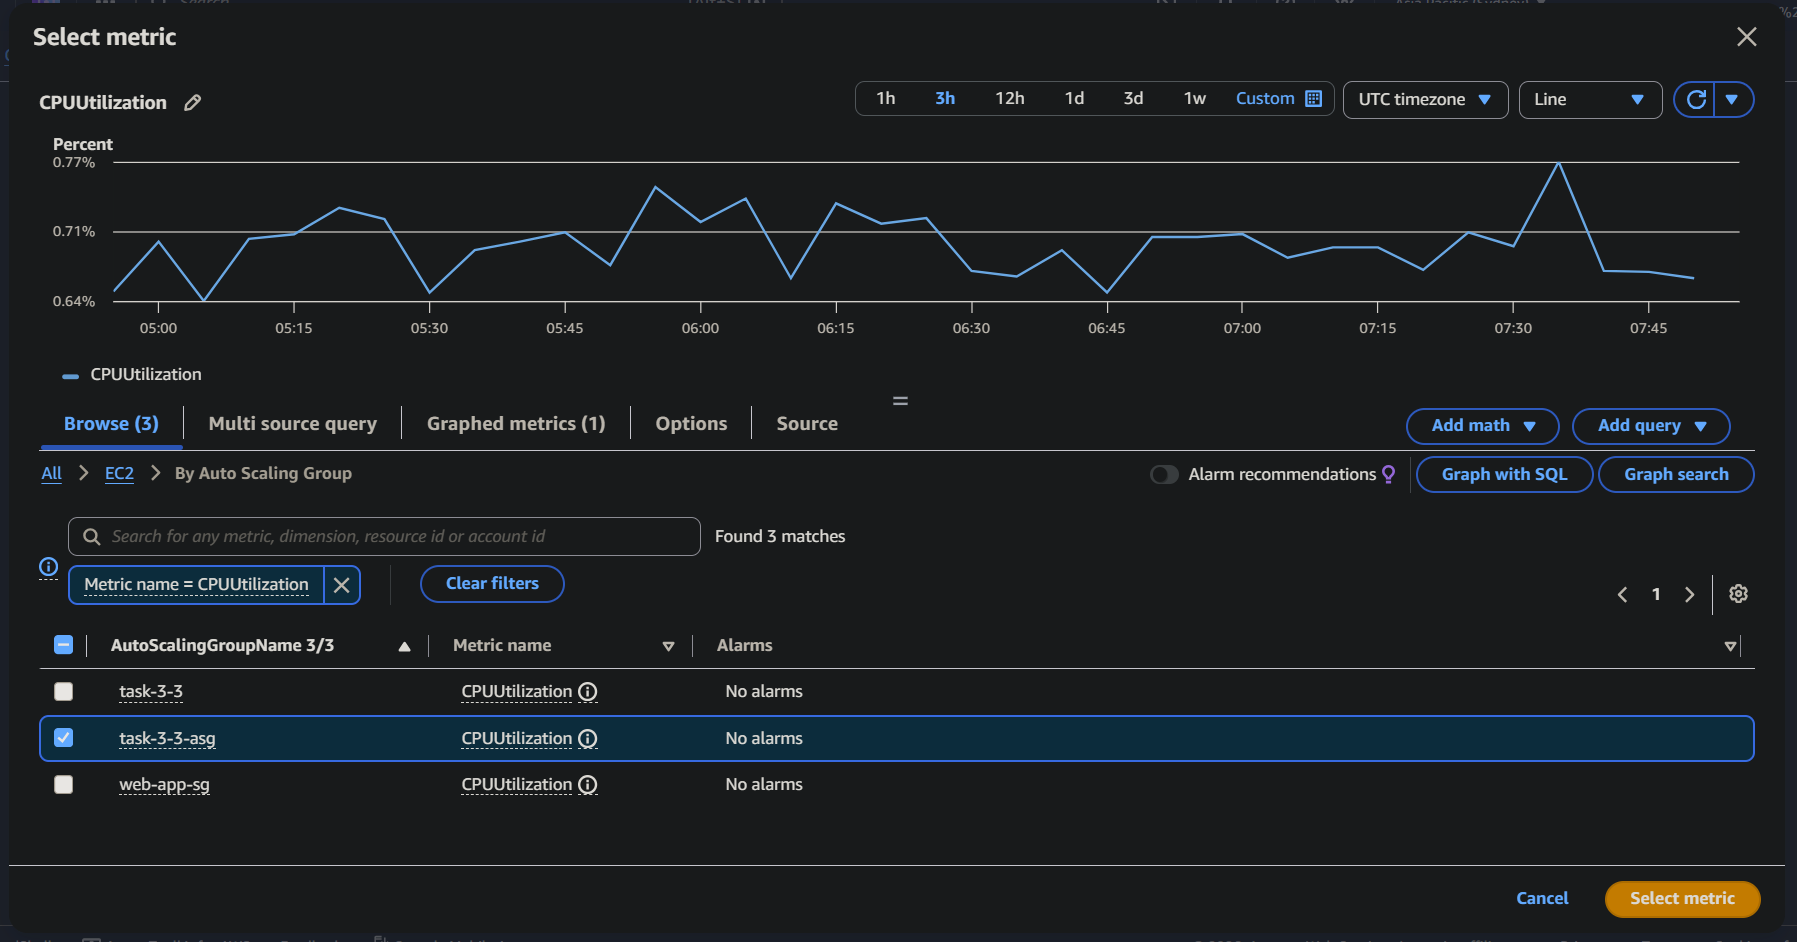
\includegraphics[scale=0.4]{images/4_select_metric.jpg}
\vspace{-1em}
\caption{Selecting the \texttt{CPUUtilization} metric for my ASG \texttt{task-3-3}.}
\end{figure}

\begin{figure}[H]
\centering
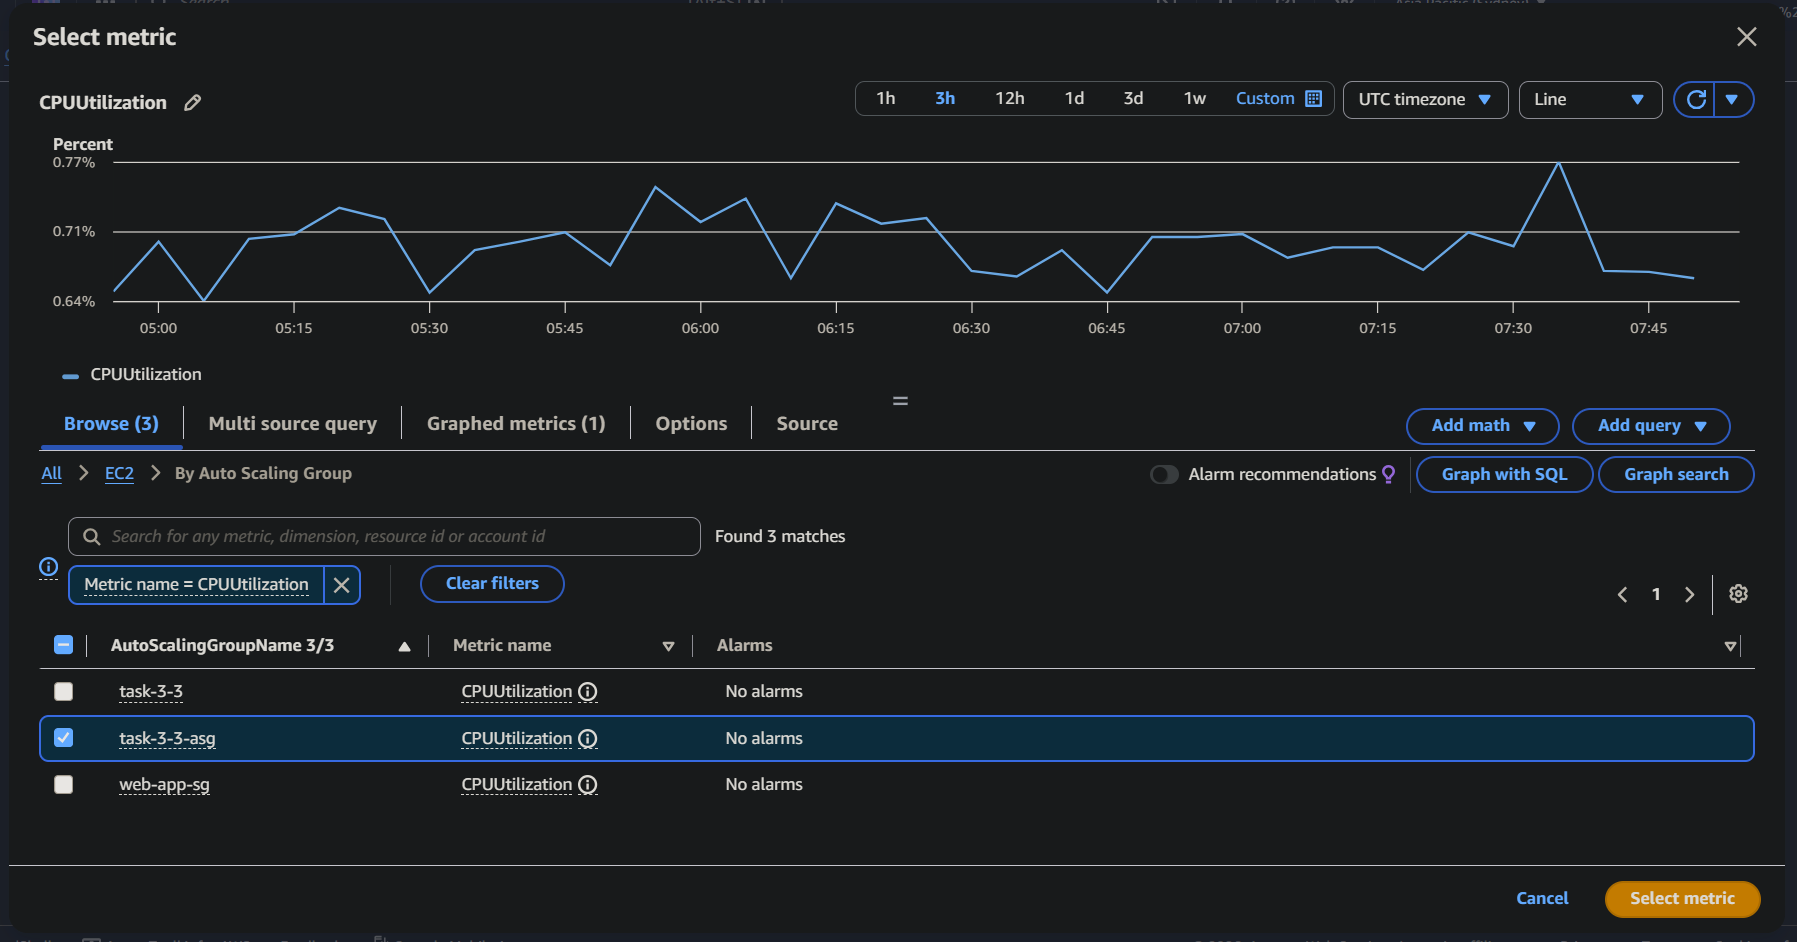
\includegraphics[scale=0.4]{images/4_select_metric.jpg}
\vspace{-1em}
\caption{Configuring the threshold for the metric to "greater than 70\%".}
\end{figure}

As previously mentioned, the SNS topic \texttt{task-3-4-topic} is attached to the alarm so that I could be notified when the average CPU utilisation metric goes past the defined threshold.

\begin{figure}[H]
\centering
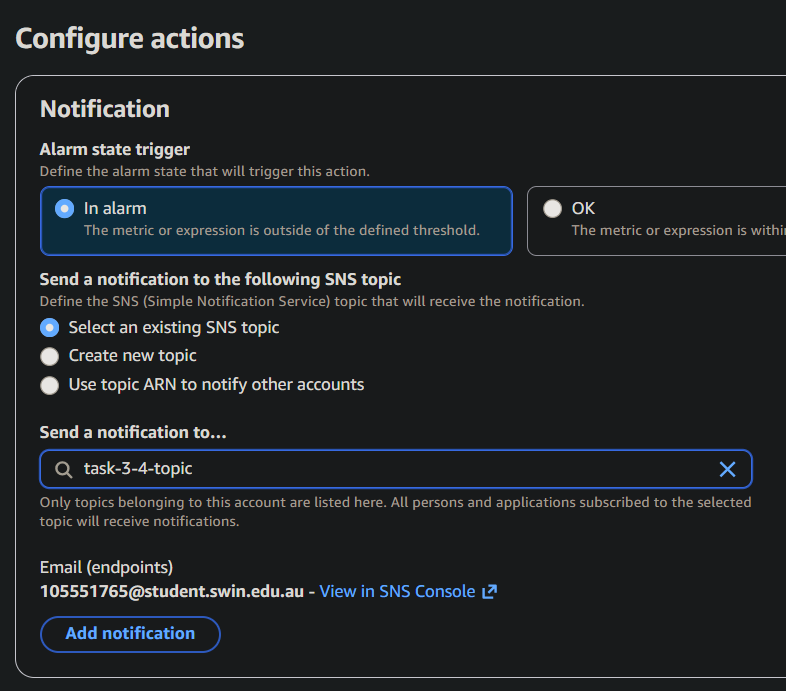
\includegraphics[scale=0.5]{images/4_config_alarm.jpg}
\vspace{-1em}
\caption{Configuring the metric to Average over a 5-minute period, with the threshold set to Greater than a value of 70.}
\end{figure}

The alarm has been created. The graph displays the defined threshold as a red dotted line against the current CPU utilisation.

\begin{figure}[H]
\centering
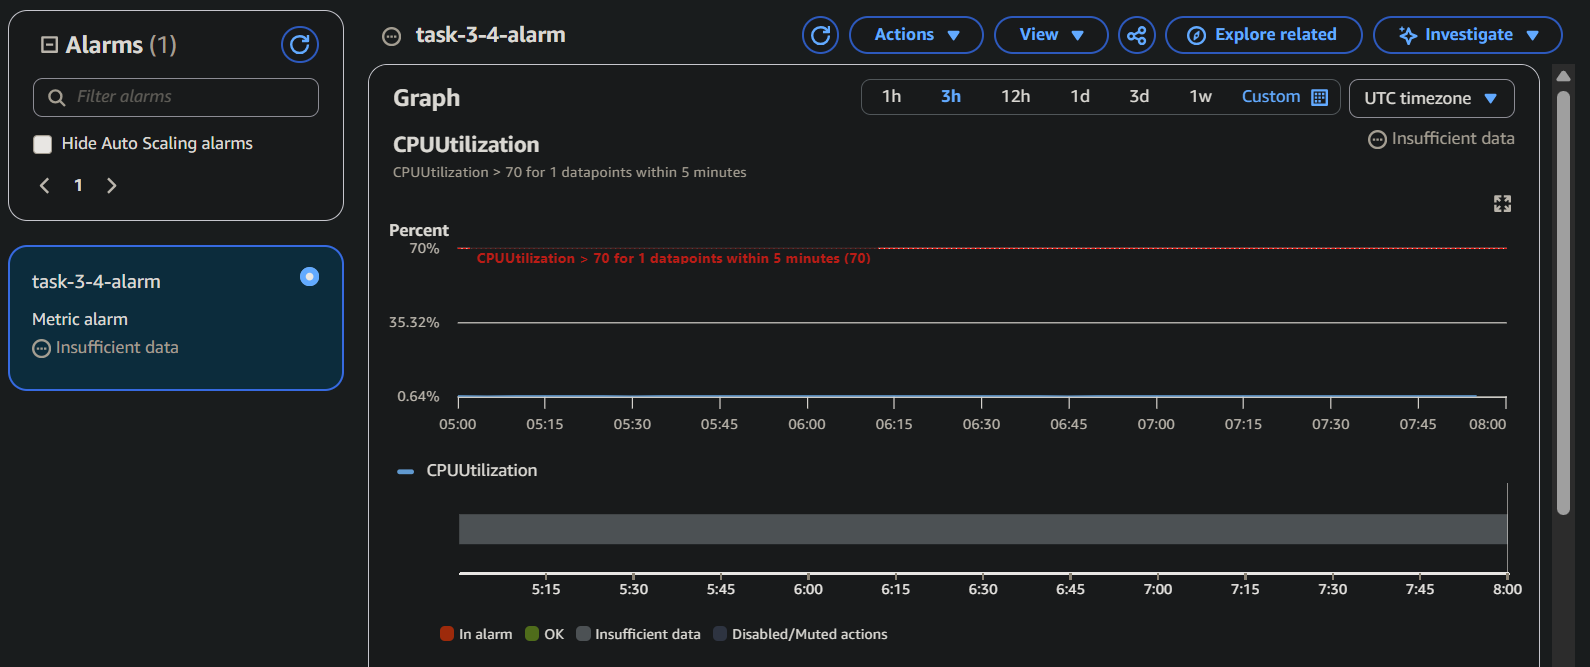
\includegraphics[scale=0.4]{images/4_metric.jpg}
\vspace{-1em}
\caption{The \texttt{task-3-4-alarm} dashboard.}
\end{figure}

\subsubsection{Secure Management via SSM}

The goal of this task is to securely access the backend EC2 instances without requiring a private key file or exposting port 22 to the public internet. The first step was to ensure that the EC2 instances had access to the AWS Systems Manager service. This was achieved by attaching the \texttt{AmazonSSMManagedInstanceCore} to their IAM role.

I attached this policy to the existing IAM role that was already associated with my EC2 instances. 

\begin{figure}[H]
\centering
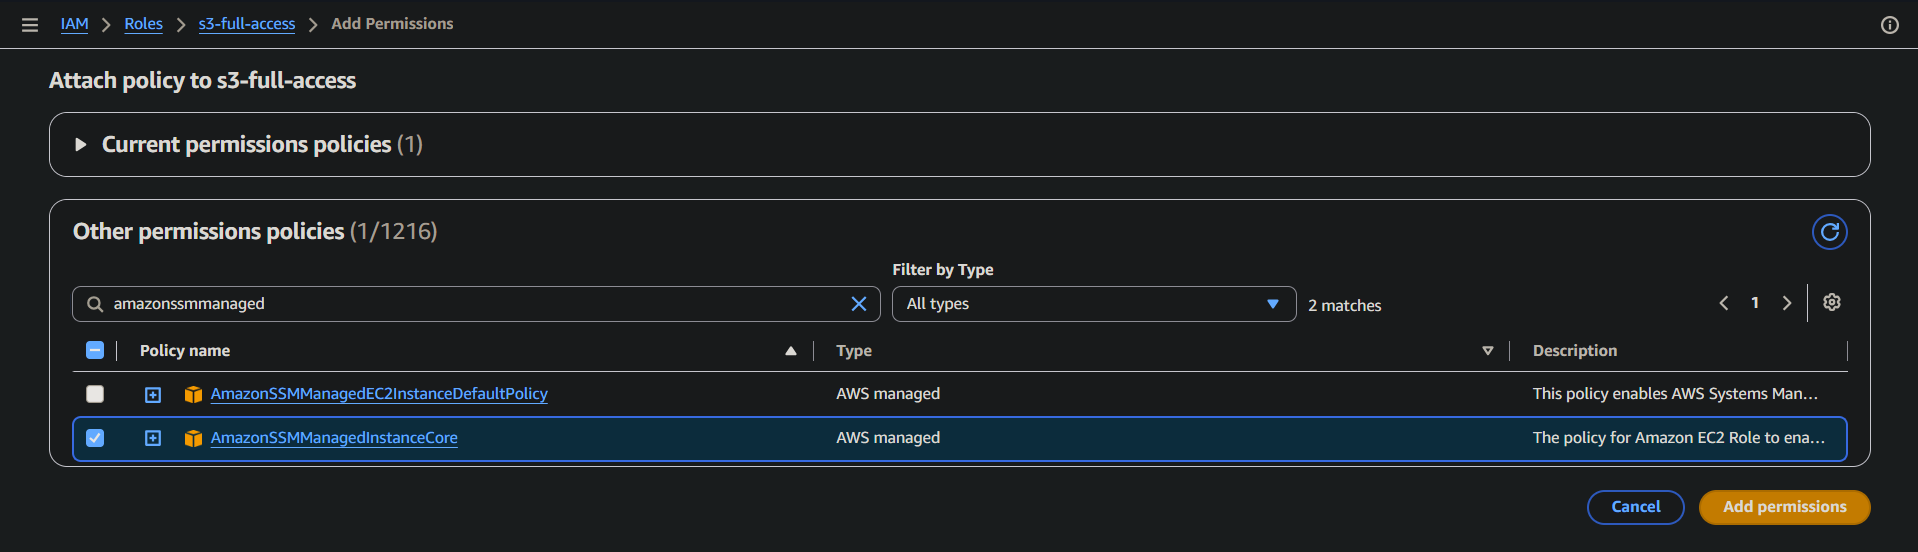
\includegraphics[scale=0.4]{images/4_add_policy.jpg}
\vspace{-1em}
\caption{Attaching the policy \texttt{AmazonSSMManagedInstanceCore} to the existing IAM role \texttt{s3-full-access} (I should've picked a better role name, in retrospect).}
\end{figure}

As an additional verification step, I SSH-ed into one of the instances to confirm that the SSM agent had already been installed. This is expected, as the SSM agent should be pre-installed on Amazon Linux instances.

\begin{figure}[H]
\centering
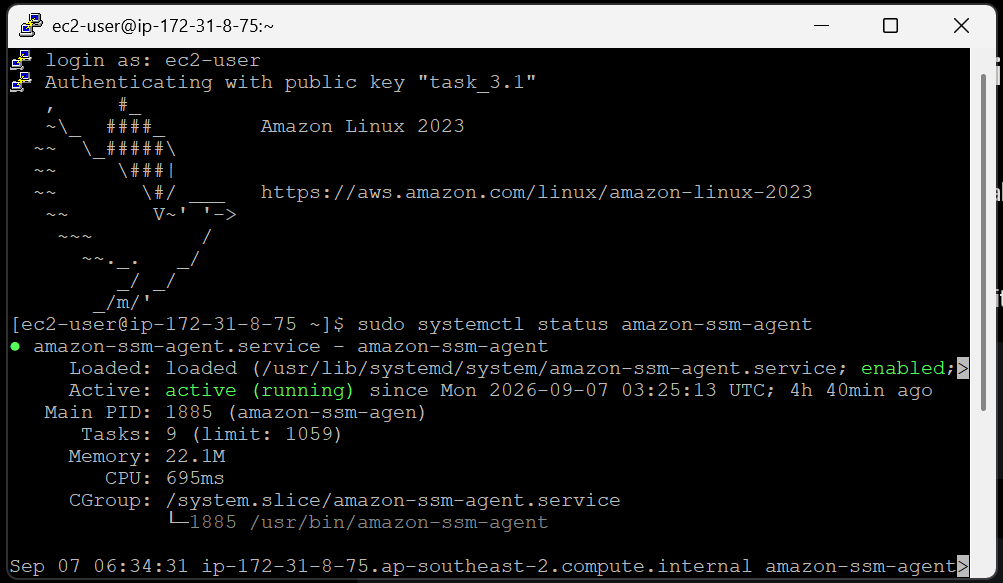
\includegraphics[scale=0.5]{images/4_confirm_agent.jpg}
\vspace{-1em}
\caption{Verifying that the SSM agent already exists on the backend EC2 instances.}
\end{figure}

Once the role has been modified, the instances are now connected to the Session Manager.

\begin{figure}[H]
\centering
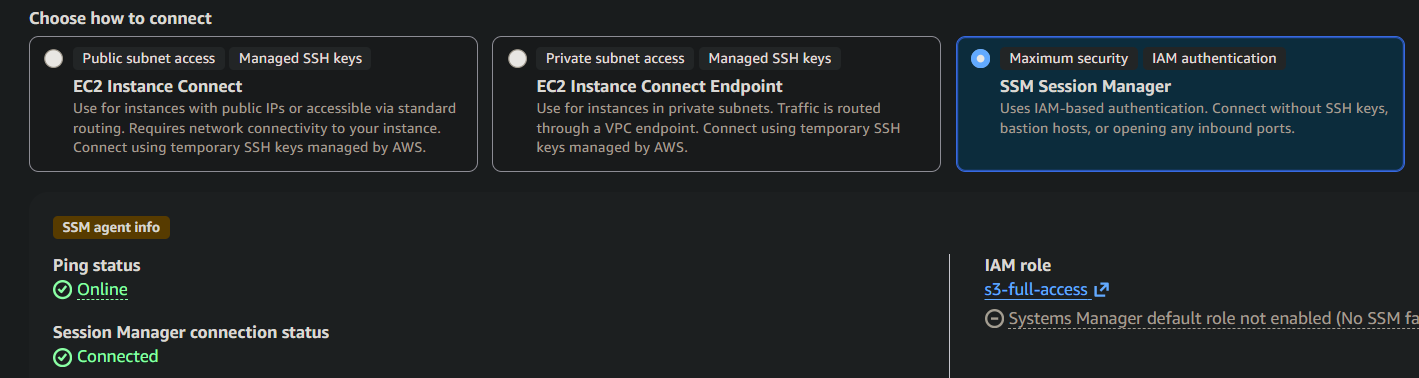
\includegraphics[scale=0.4]{images/4_ssm_connected.jpg}
\vspace{-1em}
\caption{The details of the instance \texttt{i-0f8e63855d89f9843} show that it is connected to the Session Manager.}
\end{figure}

As a proof of concept, I removed the inbound security rule which allowed public SSH access to the EC2 instances. An attempt to SSH into the instance above using PuTTY timed out following this removal. 

\begin{figure}[H]
\centering
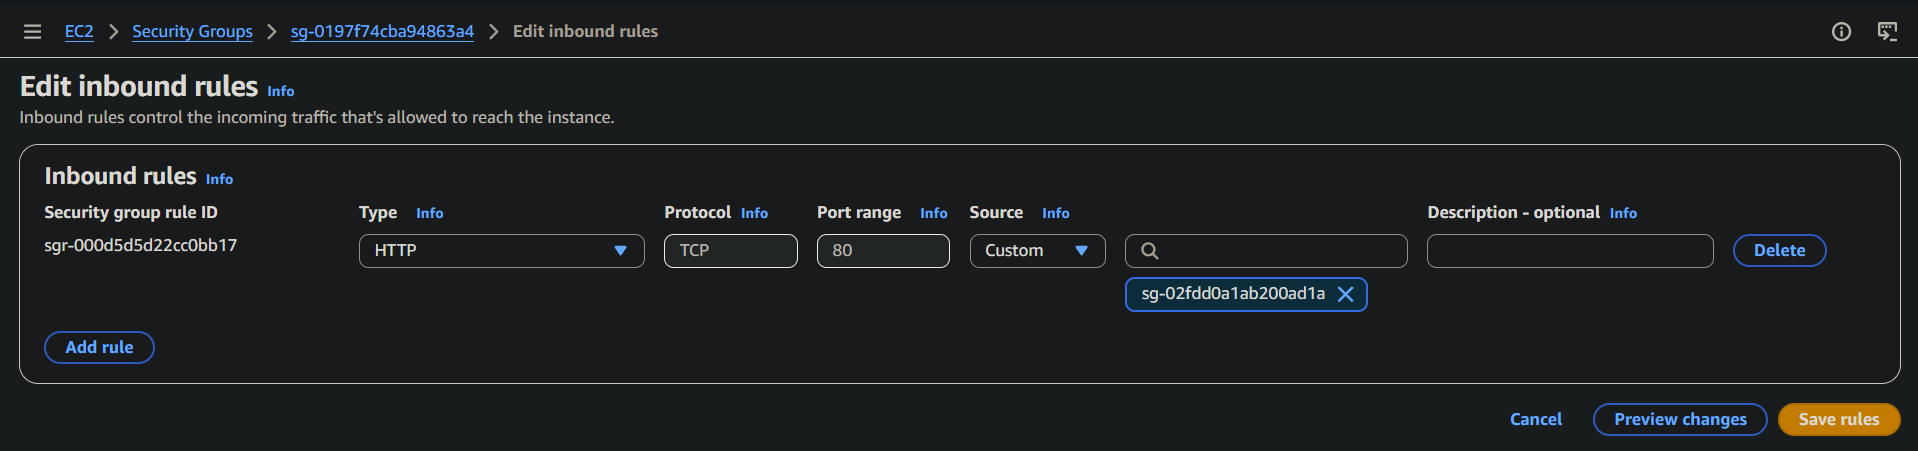
\includegraphics[scale=0.4]{images/4_edit_sg.jpg}
\vspace{-1em}
\caption{Editing the instances' security group to remove public SSH access.}
\end{figure}

\begin{figure}[H]
\centering
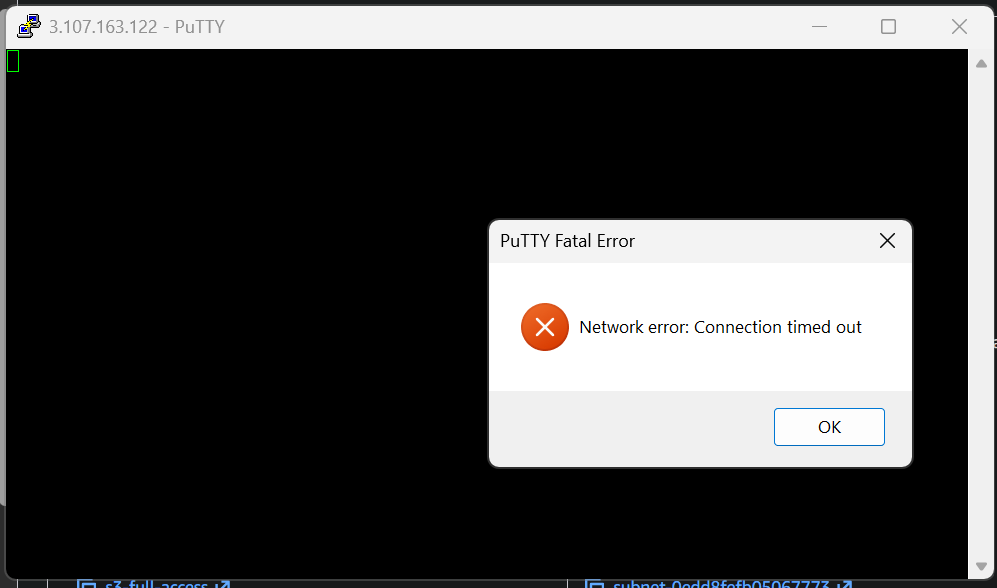
\includegraphics[scale=0.4]{images/4_timeout.jpg}
\vspace{-1em}
\caption{An attempt to SSH into the instance using PuTTY failed.}
\end{figure}

I then established a connection to the EC2 instance using the Session Manager through the AWS Console to demonstrate that I could securely access the instance's terminal without requiring an SSH connection or the use of a private key.

\begin{figure}[H]
\centering
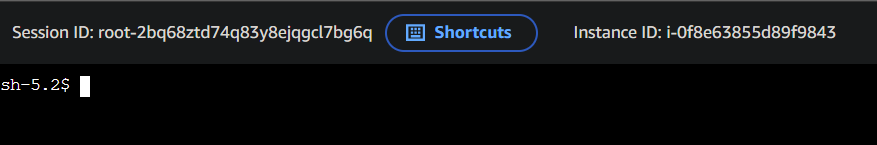
\includegraphics[scale=0.6]{images/4_ssm_terminal.jpg}
\vspace{-1em}
\caption{The Session Manager terminal session for the instance \texttt{i-0f8e63855d89f9843}.}
\end{figure}

\section{Self-troubleshooting}

% References
% \printbibliography
\end{document}